\documentclass[10pt,a4paper,twoside]{report}

\usepackage{graphicx, caption}
\usepackage{url}
\usepackage{subcaption}
\graphicspath{{Figures/} {Figures/system/} {Figures/android/} {Figures/gear/testes_bvp} {Figures/gear/} {Figures/gear_hospital/}}
\usepackage{geometry}
\usepackage{multirow}
\usepackage{placeins}
\usepackage{enumitem}
\usepackage[utf8]{inputenc}
\usepackage[english]{babel}
\usepackage{textcomp}
\usepackage{makeidx}
\usepackage{amsmath} %characteres especias math
\usepackage{hyperref} %faz as referencias
\hypersetup{colorlinks,       % color text of links and anchors,
	% eliminates borders around links
	%            linkcolor=red,    % color for normal internal links
	linkcolor=black,  % color for normal internal links
	anchorcolor=black,% color for anchor text
	%            citecolor=green,  % color for bibliographical citations
	citecolor=black,  % color for bibliographical citations
	%            filecolor=magenta,% color for URLs which open local files
	filecolor=black,  % color for URLs which open local files
	%            menucolor=red,    % color for Acrobat menu items
	menucolor=black,  % color for Acrobat menu items
	%            pagecolor=red,    % color for links to other pages
	pagecolor=black,  % color for links to other pages
	%            urlcolor=cyan,    % color for linked URLs
	urlcolor=black,   % color for linked URLs
	bookmarks=true,         % create PDF bookmarks
	bookmarksopen=false,    % don't expand bookmarks
	bookmarksnumbered=true, % number bookmarks
	pdftitle={Thesis},
	pdfauthor={Andre C. Marta},
	pdfsubject={Thesis Title},
	pdfkeywords={Thesis Keywords},
	pdfstartview=FitV,
	pdfdisplaydoctitle=true}
\usepackage{cleveref} %faz as referencias
\usepackage{titlesec} %define os espaçamentos dos cabeçalhos
\usepackage{cite} %faz a bibliografia
\usepackage{array}
\usepackage{listings}
\usepackage{color}

\geometry{verbose,tmargin=2.5cm,bmargin=2.5cm,lmargin=2.5cm,rmargin=2.5cm}


\usepackage{setspace}
\renewcommand{\baselinestretch}{1.5}


\definecolor{pblue}{rgb}{0.13,0.13,1}
\definecolor{pgreen}{rgb}{0,0.5,0}
\definecolor{pred}{rgb}{0.9,0,0}
\definecolor{pgrey}{rgb}{0.46,0.45,0.48}

\lstset{
	basicstyle=\footnotesize\tt,        % the size of the fonts that are used for the code
	breakatwhitespace=false,         % sets if automatic breaks should only happen at whitespace
	breaklines=true,                 % sets automatic line breaking
	captionpos=b,                    % sets the caption-position to bottom
	extendedchars=true,              % lets you use non-ASCII characters; for 8-bits encodings only, does not work with UTF-8
	frame=single,                    % adds a frame around the code
	language=Java,                 % the language of the code
	keywordstyle=\bf,
	showspaces=false,                % show spaces everywhere adding particular underscores; it overrides 'showstringspaces'
	showstringspaces=false,          % underline spaces within strings only
	showtabs=false,                  % show tabs within strings adding particular underscores
	tabsize=2,                       % sets default tabsize to 2 spaces
	commentstyle=\color{pgreen},
	keywordstyle=\color{pblue},
	stringstyle=\color{pred},
	moredelim=[il][\textcolor{pgrey}]{$$$$},
	moredelim=[is][\textcolor{pgrey}]{\%\%}{\%\%}
}
\definecolor{mygray}{rgb}{0.4,0.4,0.4}
\definecolor{mygreen}{rgb}{0,0.8,0.6}
\definecolor{myorange}{rgb}{1.0,0.4,0}

\lstset{
	language=C++,
	basicstyle=\footnotesize\tt,
	commentstyle=\color{mygray},
	frame=single,
	numbers=left,
	numbersep=5pt,
	numberstyle=\tiny\color{mygray},
	keywordstyle=\color{mygreen},
	showspaces=false,
	showstringspaces=false,
	stringstyle=\color{myorange},
	tabsize=2
}
%\lstset{language=C++,
%	keywordstyle=\color{blue},
%	stringstyle=\color{red},
%	commentstyle=\color{green},
%	tabsize=2,
%	morecomment=[l][\color{magenta}]{\#}
%}

\titleformat{\chapter}{\bfseries\huge}{\thechapter.}{12pt}{}
\titlespacing*{\chapter}{0pt}{-35pt}{10pt}

\newenvironment{conditions}
{\par\vspace{\abovedisplayskip}\noindent\begin{tabular}{>{$}l<{$} @{${} \rightarrow {}$} l}}
	{\end{tabular}\par\vspace{\belowdisplayskip}}


\newcommand{\acknowledgments}{@undefined} % new LaTeX variable name
\addto\captionsenglish{\renewcommand{\acknowledgments}{Acknowledgments}}
%\addto\captionsenglish{\renewcommand{\contentsname}{Contents}}
%\addto\captionsenglish{\renewcommand{\listtablename}{List of Tables}}
%\addto\captionsenglish{\renewcommand{\listfigurename}{List of Figures}}
%\addto\captionsenglish{\renewcommand{\nomname}{Nomenclature}}
%\addto\captionsenglish{\renewcommand{\glossaryname}{Glossary}}
%\addto\captionsenglish{\renewcommand{\acronymname}{List of Acronyms}}
%\addto\captionsenglish{\renewcommand{\bibname}{References}} % Bibliography
%\addto\captionsenglish{\renewcommand{\appendixname}{Appendix}}

\newcommand{\coverThesis}{@undefined} % new LaTeX variable name
\newcommand{\coverSupervisors}{@undefined} % new LaTeX variable name
\newcommand{\coverExaminationCommittee}{@undefined} % new LaTeX variable name
\newcommand{\coverChairperson}{@undefined} % new LaTeX variable name
\newcommand{\coverSupervisor}{@undefined} % new LaTeX variable name
\newcommand{\coverMemberCommittee}{@undefined} % new LaTeX variable name
% > English
\addto\captionsenglish{\renewcommand{\coverThesis}{Thesis to obtain the Master of Science Degree in}}
\addto\captionsenglish{\renewcommand{\coverSupervisors}{Supervisor(s)}}
\addto\captionsenglish{\renewcommand{\coverExaminationCommittee}{Examination Committee}}
\addto\captionsenglish{\renewcommand{\coverChairperson}{Chairperson}}
\addto\captionsenglish{\renewcommand{\coverSupervisor}{Supervisor}}
\addto\captionsenglish{\renewcommand{\coverMemberCommittee}{Member of the Committee}}
% > Portuguese
\addto\captionsportuguese{\renewcommand{\coverThesis}{Disserta\c{c}\~{a}o para obten\c{c}\~{a}o do Grau de Mestre em}}
\addto\captionsportuguese{\renewcommand{\coverSupervisors}{Orientador(es)}}
\addto\captionsportuguese{\renewcommand{\coverExaminationCommittee}{J\'{u}ri}}
\addto\captionsportuguese{\renewcommand{\coverChairperson}{Presidente}}
\addto\captionsportuguese{\renewcommand{\coverSupervisor}{Orientador}}
\addto\captionsportuguese{\renewcommand{\coverMemberCommittee}{Vogal}}

\renewcommand{\rmdefault}{phv}
\renewcommand{\sfdefault}{phv}

\def\FontLn{% 16 pt normal
	\usefont{T1}{phv}{m}{n}\fontsize{16pt}{16pt}\selectfont}
\def\FontLb{% 16 pt bold
	\usefont{T1}{phv}{b}{n}\fontsize{16pt}{16pt}\selectfont}
\def\FontMn{% 14 pt normal
	\usefont{T1}{phv}{m}{n}\fontsize{14pt}{14pt}\selectfont}
\def\FontMb{% 14 pt bold
	\usefont{T1}{phv}{b}{n}\fontsize{14pt}{14pt}\selectfont}
\def\FontSn{% 12 pt normal
	\usefont{T1}{phv}{m}{n}\fontsize{12pt}{12pt}\selectfont}

\usepackage{nomencl}
\makenomenclature
%
% Group variables according to their symbol type
%
\RequirePackage{ifthen} 
\ifthenelse{\equal{\languagename}{english}}%
{ % English
	\renewcommand{\nomgroup}[1]{%
		\ifthenelse{\equal{#1}{R}}{%
			\item[\textbf{Roman symbols}]}{%
			\ifthenelse{\equal{#1}{G}}{%
				\item[\textbf{Greek symbols}]}{%
				\ifthenelse{\equal{#1}{S}}{%
					\item[\textbf{Subscripts}]}{%
					\ifthenelse{\equal{#1}{T}}{%
						\item[\textbf{Superscripts}]}{}}}}}%
}{% Portuguese
	\renewcommand{\nomgroup}[1]{%
		\ifthenelse{\equal{#1}{R}}{%
			\item[\textbf{Simbolos romanos}]}{%
			\ifthenelse{\equal{#1}{G}}{%
				\item[\textbf{Simbolos gregos}]}{%
				\ifthenelse{\equal{#1}{S}}{%
					\item[\textbf{Subscritos}]}{%
					\ifthenelse{\equal{#1}{T}}{%
						\item[\textbf{Sobrescritos}]}{}}}}}%
}%


\usepackage{acro}
%\acsetup{list-style=tabular}
\acsetup{extra-style=comma}

\usepackage{rotating}
\usepackage[numbers]{natbib} % <<<<< References in numbered list [1],[2],...
\usepackage{notoccite}
\usepackage{booktabs}
\usepackage{pdfpages}
\newcommand{\ud}{\mathrm{d}}                % total derivative
\newcommand{\degree}{\ensuremath{^\circ\,}} % degrees
\newcommand{\mcol}{\multicolumn}            % table format

\newcommand{\eqnref}[1]{(\ref{#1})}
\newcommand{\class}[1]{\texttt{#1}}
\newcommand{\package}[1]{\texttt{#1}}
\newcommand{\file}[1]{\texttt{#1}}
\newcommand{\BibTeX}{\textsc{Bib}\TeX}

\newcommand{\tr}[1]{{\ensuremath{\textrm{#1}}}}   % text roman
\newcommand{\tb}[1]{{\ensuremath{\textbf{#1}}}}   % text bold face
\newcommand{\ti}[1]{{\ensuremath{\textit{#1}}}}   % text italic
\newcommand{\mc}[1]{{\ensuremath{\mathcal{#1}}}}  % math calygraphy
\newcommand{\mco}[1]{{\ensuremath{\mathcalold{#1}}}}% math old calygraphy
\newcommand{\mr}[1]{{\ensuremath{\mathrm{#1}}}}   % math roman
\newcommand{\mb}[1]{{\ensuremath{\mathbf{#1}}}}   % math bold face
\newcommand{\bs}[1]{\ensuremath{\boldsymbol{#1}}} % math symbol
\def\bm#1{\mathchoice                             % math bold
	{\mbox{\boldmath$\displaystyle#1$}}%
	{\mbox{\boldmath$#1$}}%
	{\mbox{\boldmath$\scriptstyle#1$}}%
	{\mbox{\boldmath$\scriptscriptstyle#1$}}}
\newcommand{\boldcal}[1]{{\ensuremath{\boldsymbol{\mathcal{#1}}}}}% math bold calygraphy

 % file "Thesis_Preamble.tex"

%%%%%%%%%%%%%%%%%%%%%%%%%%%%%%%%%%%%%%%%%%%%%%%%%%%%%%%%%%%%%%%%%%%%%%%%
%                                                                      %
%     File: Thesis_Nomenclature.tex                                    %
%     Tex Master: Thesis.tex                                           %
%                                                                      %
%     Author: Andre C. Marta                                           %
%     Last modified : 21 Jan 2011                                      %
%                                                                      %
%%%%%%%%%%%%%%%%%%%%%%%%%%%%%%%%%%%%%%%%%%%%%%%%%%%%%%%%%%%%%%%%%%%%%%%%
%
% The definitions can be placed anywhere in the document body
% and their order is sorted by <symbol> automatically when
% calling makeindex in the makefile
%
% The \glossary command has the following syntax:
%
% \glossary{entry}
%
% The \nomenclature command has the following syntax:
%
% \nomenclature[<prefix>]{<symbol>}{<description>}
%
% where <prefix> is used for fine tuning the sort order,
% <symbol> is the symbol to be described, and <description> is
% the actual description.

% ----------------------------------------------------------------------
%% Roman symbols [r]
%\nomenclature[ru]{$\bf u$}{Velocity vector.}
%\nomenclature[ru]{$u,v,w$}{Velocity Cartesian components.}
%\nomenclature[rp]{$p$}{Pressure.}
%\nomenclature[rC]{$C_D$}{Coefficient of drag.}
%\nomenclature[rC]{$C_L$}{Coefficient of lift.}
%\nomenclature[rC]{$C_M$}{Coefficient of moment.}
%
%% ----------------------------------------------------------------------
%% Greek symbols [g]
%\nomenclature[g]{$\rho$}{Density.}
%\nomenclature[g]{$\alpha$}{Angle of attack.}
%\nomenclature[g]{$\beta$}{Angle of side-slip.}
%\nomenclature[g]{$\mu$}{Molecular viscosity coefficient.}
%\nomenclature[g]{$\kappa$}{Thermal conductivity coefficient.}
%
%% ----------------------------------------------------------------------
%% Subscripts [s]
%\nomenclature[s]{$x,y,z$}{Cartesian components.}
%\nomenclature[s]{$i,j,k$}{Computational indexes.}
%\nomenclature[s]{$\infty$}{Free-stream condition.}
%\nomenclature[s]{ref}{Reference condition.}
%\nomenclature[s]{$n$}{Normal component.}
%
%% ----------------------------------------------------------------------
%% Supercripts [t]
%\nomenclature[t]{T}{Transpose.}
%\nomenclature[t]{*}{Adjoint.}

\DeclareAcronym{angelsperarea}{
	short = \ensuremath{a} ,
	long  = The number of angels per unit area ,
	sort  = a ,
	class = nomencl
}
\DeclareAcronym{numofangels}{
	short = \ensuremath{N} ,
	long  = The number of angels per needle point ,
	sort  = N ,
	class = nomencl
}
\DeclareAcronym{areaofneedle}{
	short = \ensuremath{A} ,
	long  = The area of the needle point ,
	sort  = A ,
	class = nomencl
}

%\DeclareAcronym{bpm}{
%	short = bpm ,
%	long  = Beats Per Minute ,
%	sort  = bpm ,
%	class = nomencl
%}
%
%\DeclareAcronym{sd}{
%	short = SD ,
%	long  = Secure Digital card,
%	sort  = bpm ,
%	class = nomencl
%}
%
%\DeclareAcronym{os}{
%	short = OS ,
%	long  = Operative System,
%	sort  = bpm ,
%	class = nomencl
%}



%%%%%%%%%%%%%%%%%%%%%%%%%%%%%%%%%%%%%%%%%%%%%%%%%%%%%%%%%%%%%%%%%%%%%%%%
%                                                                      %
%     File: Thesis_Glossary.tex                                        %
%     Tex Master: Thesis.tex                                           %
%                                                                      %
%     Author: Andre C. Marta                                           %
%     Last modified : 30 Oct 2012                                      %
%                                                                      %
%%%%%%%%%%%%%%%%%%%%%%%%%%%%%%%%%%%%%%%%%%%%%%%%%%%%%%%%%%%%%%%%%%%%%%%%
%
% The definitions can be placed anywhere in the document body
% and their order is sorted by <symbol> automatically when
% calling makeindex in the makefile
%
% The \glossary command has the following syntax:
%
% \glossary{entry}
%
% The \nomenclature command has the following syntax:
%
% \nomenclature[<prefix>]{<symbol>}{<description>}
%
% where <prefix> is used for fine tuning the sort order,
% <symbol> is the symbol to be described, and <description> is
% the actual description.

% ----------------------------------------------------------------------

%\glossary{name={\textbf{MDO}},description={Multi-Disciplinar Optimization is an engineering technique that uses optimization methods to solve design problems incorporating two or more disciplines.}}
%
%\glossary{name={\textbf{CFD}},description={Computational Fluid Dynamics is a branch of fluid mechanics that uses numerical methods and algorithms to solve problems that involve fluid flows.}}
%
%\glossary{name={\textbf{CSM}},description={Computational Structural Mechanics is a branch of structure mechanics that uses numerical methods and algorithms to perform the analysis of structures and its components.}}


\DeclareAcronym{ny}{
	short = NY ,
	long  = New York ,
	class = abbrev
}
\DeclareAcronym{la}{
	short = LA ,
	long  = Los Angeles ,
	class = abbrev
}
\DeclareAcronym{un}{
	short = UN ,
	long  = United Nations ,
	class = abbrev
}

\DeclareAcronym{hsm}{
	short = HSM ,
	long  = Hospital de Santa Marta - CHLC ,
	class = abbrev
}
\DeclareAcronym{hr}{
	short = HR ,
	long  = Heart Rate ,
	class = abbrev
}
\DeclareAcronym{mets}{
	short = METs ,
	long  = Metabolic Equivalent of Tasks ,
	class = abbrev
}

\DeclareAcronym{ecg}{
	short = ECG ,
	long  = electrocardiogram ,
	class = abbrev
}

\DeclareAcronym{ppg}{
	short = PPG ,
	long  = photoplethysmography ,
	class = abbrev
}

\DeclareAcronym{bt}{
	short = BT ,
	long  = Bluetooth ,
	class = abbrev
}

\DeclareAcronym{uuid}{
	short = UUID ,
	long  = Universally Unique Identifier  ,
	class = abbrev
}

\DeclareAcronym{ui}{
	short = UI ,
	long  = User Interface  ,
	class = abbrev
}

\DeclareAcronym{insticc}{
	short = INSTICC ,
	long  = \text{Institute for Systems and Technologies of Information, Control and Communication}  ,
	class = abbrev
}

\DeclareAcronym{rp}{
	short = RP ,
	long  = \text{R-peaks, the point with largest amplitude in QRS complex} ,
	class = abbrev
}

\DeclareAcronym{acc}{
	short = ACC ,
	long  = Accelerometry ,
	class = abbrev
}

\DeclareAcronym{bpm}{
	short = bpm ,
	long  = Beats Per Minute ,
	sort  = bpm ,
	class = abbrev
}

\DeclareAcronym{sd}{
	short = SD ,
	long  = Secure Digital card,
	sort  = sd ,
	class = abbrev
}

\DeclareAcronym{os}{
	short = OS ,
	long  = Operative System,
	sort  = os ,
	class = abbrev
}

\DeclareAcronym{bvp}{
	short = BVP ,
	long  = Blood Volume Pulse,
	sort  = bvp ,
	class = abbrev
}

\DeclareAcronym{pda}{
	short = PDA ,
	long  = Personal Digital Assistant,
	sort  = pda ,
	class = abbrev
}

\DeclareAcronym{rf}{
	short = RF ,
	long  = Rado Frequency,
	sort  = rf ,
	class = abbrev
}

\DeclareAcronym{bsn}{
	short = BSN ,
	long  = Body Sensor Network,
	sort  = bsn ,
	class = abbrev
}

\DeclareAcronym{qrs}{
	short = QRS ,
	long  = ECG wave QRS complex,
	sort  = bsn ,
	class = abbrev
}


\DeclareAcronym{led}{
	short = LED ,
	long  = Light Emitting Diode,
	sort  = led ,
	class = abbrev
}

\DeclareAcronym{snr}{
short = SNR ,
long  = Signal to Noise Ratio,
sort  = snr ,
class = abbrev
}

\DeclareAcronym{fft}{
	short = FFT ,
	long  = Fast Fourier Transform,
	sort  = fft ,
	class = abbrev
}

\DeclareAcronym{gsm}{
	short = GSM ,
	long  = Global System for Mobile Communications,
	sort  = gsm ,
	class = abbrev
}



\begin{document}

\pagestyle{plain}

% Set roman numbering (i,ii,...) before the start of chapters
\pagenumbering{roman}

%%%%%%%%%%%%%%%%%%%%%%%%%%%%%%%%%%%%%%%%%%%%%%%%%%%%%%%%%%%%%%%%%%%%%%%%
%                                                                      %
%     File: Thesis_FrontCover.tex                                      %
%     Tex Master: Thesis.tex                                           %
%                                                                      %
%     Author: Andre C. Marta                                           %
%     Last modified :  2 Jul 2015                                      %
%                                                                      %
%%%%%%%%%%%%%%%%%%%%%%%%%%%%%%%%%%%%%%%%%%%%%%%%%%%%%%%%%%%%%%%%%%%%%%%%

\thispagestyle {empty}

% IST Logo - Signature A
% parameters: bb=llx lly urx ury (bounding box), width=h_length, height=v_length, angle=angle, scale=factor, clip=true/false, draft=true/false. 

\includegraphics[bb=9.5cm 11cm 0cm 0cm,scale=0.29]{IST_A_CMYK_POS}

\begin{center}
%
% Figure (Image or plot)
\vspace{2.5cm}
% height = 50 mm
%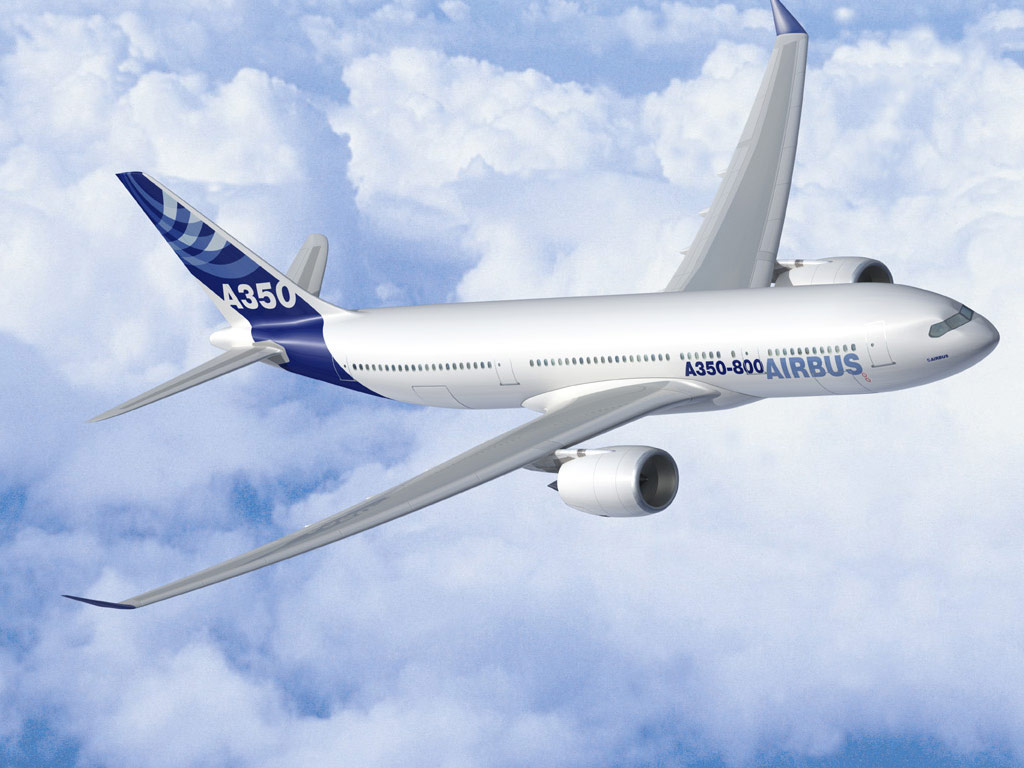
\includegraphics[height=50mm]{Figures/Airbus_A350.jpg}

% Title, author and degree
\vspace{1.0cm}
{\FontLb Long Term Real-Time Pervasive Monitoring System for non-Hospitalized Patients} \\ % <<<<< EDIT TITLE
%\vspace{0.2cm}
%{\FontMn Subtitle (optional)} \\
%\vspace{1.9cm}
\vspace{2.0cm}
{\FontMb André Ferreira Manso} \\ % <<<<< EDIT NAME
\vspace{2.0cm}
{\FontSn \coverThesis} \\
\vspace{0.3cm}
{\FontLb Biomedical Engineering} \\ % <<<<< EDIT COURSE
\vspace{1.0cm}
{\FontSn %
\begin{tabular}{ll}
 \coverSupervisors: & Prof. Ana Luisa Nobre Fred \\ % <<<<< EDIT NAME
                    & Dr. Rui Cruz Ferreira    % <<<<< EDIT NAME
\end{tabular} } \\
\vspace{1.0cm}
{\FontMb \coverExaminationCommittee} \\
\vspace{0.3cm}
{\FontSn %
\begin{tabular}{c}
\coverChairperson:     Prof. Full Name          \\ % <<<<< EDIT NAME
\coverSupervisor:      Prof. Full Name 1 (or 2) \\ % <<<<< EDIT NAME
\coverMemberCommittee: Prof. Full Name 3           % <<<<< EDIT NAME
\end{tabular} } \\
\vspace{1.5cm}
{\FontMb Month Year} \\ % <<<<< EDIT DATE (corresponds to date of oral examination)
%
\end{center}

 % file "Thesis_FrontCover.tex"
\cleardoublepage

%%%%%%%%%%%%%%%%%%%%%%%%%%%%%%%%%%%%%%%%%%%%%%%%%%%%%%%%%%%%%%%%%%%%%%%%%
%                                                                      %
%     File: Thesis_Dedication.tex                                      %
%     Tex Master: Thesis.tex                                           %
%                                                                      %
%     Author: Andre C. Marta                                           %
%     Last modified :  2 Jul 2015                                      %
%                                                                      %
%%%%%%%%%%%%%%%%%%%%%%%%%%%%%%%%%%%%%%%%%%%%%%%%%%%%%%%%%%%%%%%%%%%%%%%%

\null\vskip5cm%
\begin{flushright}
     Dedicated to someone special...
\end{flushright}
\vfill\newpage

 % file "Thesis_Dedication.tex"
%\cleardoublepage

%%%%%%%%%%%%%%%%%%%%%%%%%%%%%%%%%%%%%%%%%%%%%%%%%%%%%%%%%%%%%%%%%%%%%%%%
%                                                                      %
%     File: Thesis_Acknowledgments.tex                                 %
%     Tex Master: Thesis.tex                                           %
%                                                                      %
%     Author: Andre C. Marta                                           %
%     Last modified :  2 Jul 2015                                      %
%                                                                      %
%%%%%%%%%%%%%%%%%%%%%%%%%%%%%%%%%%%%%%%%%%%%%%%%%%%%%%%%%%%%%%%%%%%%%%%%

\section*{\acknowledgments}

% Add entry in the table of contents as section
\addcontentsline{toc}{section}{\acknowledgments}

%A few words about the university, financial support, research advisor, dissertation readers, faculty or other professors, lab mates, other friends and family...

O meu primeiro agradecimento será para a Prof. Ana Fred que me convidou a participar neste projeto e me apoiou em todas as fases, esclarecendo e solucionando todas as questões que foram surgindo.

Um obrigado também ao Rui César das Neves por ter ajudado a fazer deste projeto uma realidade, e ao Filipe Mariano por ter cedido o software do projeto Telemold e ajudado á sua compreensão, sem o qual a implementação teria sido muito mais morosa e custosa.

Gostaria também de agradecer a toda a equipa do Hospital de Santa Marta pelo apoio durante a realização do projeto, em particular ao Dr. Rui Ferreira por ser um impulsionador da inovação e digitalização da medicina em Portugal, por portugueses.

Um grande obrigado também ao Hugo Silva por ter contribuído com a montagem de uns bonitos Bitalinos, por ter sempre ideias espetaculares e ter sempre uma palavra de encorajamento a dar. Novamente agradeço a Prof. Ana Fred por ter também dado um toque de estilo ao que, sem ela, seriam umas faixas muito feias.

Não poderia também deixar de agradecer a todos os amigos que me apoiaram quando precisei de ajuda ou animo. Um agradecimento especial à minha família e à minha mais que tudo por toda a ajuda, apoio e carinho que me deram no decorrer destes meses.

Finalmente, quero deixar um agradecimento ao Miguel Martinho por ter aturado os meus queixumes e ter sido parceiro e alicerce em incontáveis brainstorms e aventuras. 

%\textcolor{red}{\Large \textbf{Filipe Mariano/INSTICC - software, hugo silva - faixa}}

 % file "Thesis_Acknowledgements.tex"
\cleardoublepage

%%%%%%%%%%%%%%%%%%%%%%%%%%%%%%%%%%%%%%%%%%%%%%%%%%%%%%%%%%%%%%%%%%%%%%%%
%                                                                      %
%     File: Thesis_Resumo.tex                                          %
%     Tex Master: Thesis.tex                                           %
%                                                                      %
%     Author: Andre C. Marta                                           %
%     Last modified :  2 Jul 2015                                      %
%                                                                      %
%%%%%%%%%%%%%%%%%%%%%%%%%%%%%%%%%%%%%%%%%%%%%%%%%%%%%%%%%%%%%%%%%%%%%%%%

\section*{Resumo}

% Add entry in the table of contents as section
\addcontentsline{toc}{section}{Resumo}

Igual ao Abstract

\vfill

\textbf{\Large Palavras-chave:} palavra-chave1, palavra-chave2,...

   % file "Thesis_Resumo.tex"
\cleardoublepage

%%%%%%%%%%%%%%%%%%%%%%%%%%%%%%%%%%%%%%%%%%%%%%%%%%%%%%%%%%%%%%%%%%%%%%%%
%                                                                      %
%     File: Thesis_Abstract.tex                                        %
%     Tex Master: Thesis.tex                                           %
%                                                                      %
%     Author: Andre C. Marta                                           %
%     Last modified :  2 Jul 2015                                      %
%                                                                      %
%%%%%%%%%%%%%%%%%%%%%%%%%%%%%%%%%%%%%%%%%%%%%%%%%%%%%%%%%%%%%%%%%%%%%%%%

\section*{Abstract}

% Add entry in the table of contents as section
\addcontentsline{toc}{section}{Abstract}

In recent years, sensors and data collection devices have become an ever more ubiquitous presence. This has a major potential concerning medical procedures, opening the path for personalized medicine and allowing for a more targeted and efficient diagnose and therapeutic.

In this work a novel pervasive monitoring system is proposed. It is designed to allow constant and long-term acquisition of any desired variables and visualize the signals remotely in real time via a web interface. The system is implemented to be completely versatile concerning the sensors it can interact with.

System’s functioning is based in two components, a smartphone app and a central server. The smartphone is responsible for connecting with all sensors via Bluetooth and processing, storing and relaying all data to the server. The later is responsible for long-term storing of the data, and for serving a web interface where acquisition parameters can be configured and data can be visualized through an interactive view.

The system was tested in collaboration with cardiology department of Hospital de Santa Marta – CHLC. Tests consisted in utilizing the system with two devices, a BITalino and a Samsung Gear S3 smartwatch, to monitor patient’s heart rate and physical activity, being patient’s comfort and system’s scalability important factors in device choice.

The conducted tests allowed to get feedback from all intended users: patients, physicians and medical staff. They all reported the system as being easy to interact with and very useful in getting medically relevant data, with the easy inclusion of new sensors as a major advantage.



\vfill

\textbf{\Large Keywords:} Personalized Medicine, Pervasive Monitoring, Wearable sensors, Smart devices, Bio-signals

 % file "Thesis_Abstract.tex"
\cleardoublepage

\tableofcontents
\cleardoublepage 

\phantomsection
\addcontentsline{toc}{section}{\listtablename}
% Generate list
\listoftables
\cleardoublepage 


\phantomsection
\addcontentsline{toc}{section}{\listfigurename}
% Generate list
\listoffigures
\cleardoublepage 


%%%%%%%%%%%%%%%%%%%%%%%%%%%%%%%%%%%%%%%%%%%%%%%%%%%%%%%%%%%%%%%%%%%%%%%%%
%                                                                      %
%     File: Thesis_Nomenclature.tex                                    %
%     Tex Master: Thesis.tex                                           %
%                                                                      %
%     Author: Andre C. Marta                                           %
%     Last modified : 21 Jan 2011                                      %
%                                                                      %
%%%%%%%%%%%%%%%%%%%%%%%%%%%%%%%%%%%%%%%%%%%%%%%%%%%%%%%%%%%%%%%%%%%%%%%%
%
% The definitions can be placed anywhere in the document body
% and their order is sorted by <symbol> automatically when
% calling makeindex in the makefile
%
% The \glossary command has the following syntax:
%
% \glossary{entry}
%
% The \nomenclature command has the following syntax:
%
% \nomenclature[<prefix>]{<symbol>}{<description>}
%
% where <prefix> is used for fine tuning the sort order,
% <symbol> is the symbol to be described, and <description> is
% the actual description.

% ----------------------------------------------------------------------
%% Roman symbols [r]
%\nomenclature[ru]{$\bf u$}{Velocity vector.}
%\nomenclature[ru]{$u,v,w$}{Velocity Cartesian components.}
%\nomenclature[rp]{$p$}{Pressure.}
%\nomenclature[rC]{$C_D$}{Coefficient of drag.}
%\nomenclature[rC]{$C_L$}{Coefficient of lift.}
%\nomenclature[rC]{$C_M$}{Coefficient of moment.}
%
%% ----------------------------------------------------------------------
%% Greek symbols [g]
%\nomenclature[g]{$\rho$}{Density.}
%\nomenclature[g]{$\alpha$}{Angle of attack.}
%\nomenclature[g]{$\beta$}{Angle of side-slip.}
%\nomenclature[g]{$\mu$}{Molecular viscosity coefficient.}
%\nomenclature[g]{$\kappa$}{Thermal conductivity coefficient.}
%
%% ----------------------------------------------------------------------
%% Subscripts [s]
%\nomenclature[s]{$x,y,z$}{Cartesian components.}
%\nomenclature[s]{$i,j,k$}{Computational indexes.}
%\nomenclature[s]{$\infty$}{Free-stream condition.}
%\nomenclature[s]{ref}{Reference condition.}
%\nomenclature[s]{$n$}{Normal component.}
%
%% ----------------------------------------------------------------------
%% Supercripts [t]
%\nomenclature[t]{T}{Transpose.}
%\nomenclature[t]{*}{Adjoint.}

\DeclareAcronym{angelsperarea}{
	short = \ensuremath{a} ,
	long  = The number of angels per unit area ,
	sort  = a ,
	class = nomencl
}
\DeclareAcronym{numofangels}{
	short = \ensuremath{N} ,
	long  = The number of angels per needle point ,
	sort  = N ,
	class = nomencl
}
\DeclareAcronym{areaofneedle}{
	short = \ensuremath{A} ,
	long  = The area of the needle point ,
	sort  = A ,
	class = nomencl
}

%\DeclareAcronym{bpm}{
%	short = bpm ,
%	long  = Beats Per Minute ,
%	sort  = bpm ,
%	class = nomencl
%}
%
%\DeclareAcronym{sd}{
%	short = SD ,
%	long  = Secure Digital card,
%	sort  = bpm ,
%	class = nomencl
%}
%
%\DeclareAcronym{os}{
%	short = OS ,
%	long  = Operative System,
%	sort  = bpm ,
%	class = nomencl
%}


 % file "Thesis_Nomenclature.tex"

%\phantomsection
%\addcontentsline{toc}{section}{\nomname}
%% Insert glossary/nomenclature section produced by MakeIndex
%\printacronyms[include-classes=nomencl,name=Acronyms]
%\cleardoublepage


%%%%%%%%%%%%%%%%%%%%%%%%%%%%%%%%%%%%%%%%%%%%%%%%%%%%%%%%%%%%%%%%%%%%%%%%%
%                                                                      %
%     File: Thesis_Glossary.tex                                        %
%     Tex Master: Thesis.tex                                           %
%                                                                      %
%     Author: Andre C. Marta                                           %
%     Last modified : 30 Oct 2012                                      %
%                                                                      %
%%%%%%%%%%%%%%%%%%%%%%%%%%%%%%%%%%%%%%%%%%%%%%%%%%%%%%%%%%%%%%%%%%%%%%%%
%
% The definitions can be placed anywhere in the document body
% and their order is sorted by <symbol> automatically when
% calling makeindex in the makefile
%
% The \glossary command has the following syntax:
%
% \glossary{entry}
%
% The \nomenclature command has the following syntax:
%
% \nomenclature[<prefix>]{<symbol>}{<description>}
%
% where <prefix> is used for fine tuning the sort order,
% <symbol> is the symbol to be described, and <description> is
% the actual description.

% ----------------------------------------------------------------------

%\glossary{name={\textbf{MDO}},description={Multi-Disciplinar Optimization is an engineering technique that uses optimization methods to solve design problems incorporating two or more disciplines.}}
%
%\glossary{name={\textbf{CFD}},description={Computational Fluid Dynamics is a branch of fluid mechanics that uses numerical methods and algorithms to solve problems that involve fluid flows.}}
%
%\glossary{name={\textbf{CSM}},description={Computational Structural Mechanics is a branch of structure mechanics that uses numerical methods and algorithms to perform the analysis of structures and its components.}}


\DeclareAcronym{ny}{
	short = NY ,
	long  = New York ,
	class = abbrev
}
\DeclareAcronym{la}{
	short = LA ,
	long  = Los Angeles ,
	class = abbrev
}
\DeclareAcronym{un}{
	short = UN ,
	long  = United Nations ,
	class = abbrev
}

\DeclareAcronym{hsm}{
	short = HSM ,
	long  = Hospital de Santa Marta - CHLC ,
	class = abbrev
}
\DeclareAcronym{hr}{
	short = HR ,
	long  = Heart Rate ,
	class = abbrev
}
\DeclareAcronym{mets}{
	short = METs ,
	long  = Metabolic Equivalent of Tasks ,
	class = abbrev
}

\DeclareAcronym{ecg}{
	short = ECG ,
	long  = electrocardiogram ,
	class = abbrev
}

\DeclareAcronym{ppg}{
	short = PPG ,
	long  = photoplethysmography ,
	class = abbrev
}

\DeclareAcronym{bt}{
	short = BT ,
	long  = Bluetooth ,
	class = abbrev
}

\DeclareAcronym{uuid}{
	short = UUID ,
	long  = Universally Unique Identifier  ,
	class = abbrev
}

\DeclareAcronym{ui}{
	short = UI ,
	long  = User Interface  ,
	class = abbrev
}

\DeclareAcronym{insticc}{
	short = INSTICC ,
	long  = \text{Institute for Systems and Technologies of Information, Control and Communication}  ,
	class = abbrev
}

\DeclareAcronym{rp}{
	short = RP ,
	long  = \text{R-peaks, the point with largest amplitude in QRS complex} ,
	class = abbrev
}

\DeclareAcronym{acc}{
	short = ACC ,
	long  = Accelerometry ,
	class = abbrev
}

\DeclareAcronym{bpm}{
	short = bpm ,
	long  = Beats Per Minute ,
	sort  = bpm ,
	class = abbrev
}

\DeclareAcronym{sd}{
	short = SD ,
	long  = Secure Digital card,
	sort  = sd ,
	class = abbrev
}

\DeclareAcronym{os}{
	short = OS ,
	long  = Operative System,
	sort  = os ,
	class = abbrev
}

\DeclareAcronym{bvp}{
	short = BVP ,
	long  = Blood Volume Pulse,
	sort  = bvp ,
	class = abbrev
}

\DeclareAcronym{pda}{
	short = PDA ,
	long  = Personal Digital Assistant,
	sort  = pda ,
	class = abbrev
}

\DeclareAcronym{rf}{
	short = RF ,
	long  = Rado Frequency,
	sort  = rf ,
	class = abbrev
}

\DeclareAcronym{bsn}{
	short = BSN ,
	long  = Body Sensor Network,
	sort  = bsn ,
	class = abbrev
}

\DeclareAcronym{qrs}{
	short = QRS ,
	long  = ECG wave QRS complex,
	sort  = bsn ,
	class = abbrev
}


\DeclareAcronym{led}{
	short = LED ,
	long  = Light Emitting Diode,
	sort  = led ,
	class = abbrev
}

\DeclareAcronym{snr}{
short = SNR ,
long  = Signal to Noise Ratio,
sort  = snr ,
class = abbrev
}

\DeclareAcronym{fft}{
	short = FFT ,
	long  = Fast Fourier Transform,
	sort  = fft ,
	class = abbrev
}

\DeclareAcronym{gsm}{
	short = GSM ,
	long  = Global System for Mobile Communications,
	sort  = gsm ,
	class = abbrev
}

 % file "Thesis_Glossary.tex"


\phantomsection
\addcontentsline{toc}{section}{\glossaryname}
\printacronyms[name=Acronyms]
\cleardoublepage

\setcounter{page}{1}
\pagenumbering{arabic}


%%%%%%%%%%%%%%%%%%%%%%%%%%%%%%%%%%%%%%%%%%%%%%%%%%%%%%%%%%%%%%%%%%%%%%%%
%                                                                      %
%     File: Thesis_Introduction.tex                                    %
%     Tex Master: Thesis.tex                                           %
%                                                                      %
%     Author: Andre C. Marta                                           %
%     Last modified :  2 Jul 2015                                      %
%                                                                      %
%%%%%%%%%%%%%%%%%%%%%%%%%%%%%%%%%%%%%%%%%%%%%%%%%%%%%%%%%%%%%%%%%%%%%%%%

\chapter{Introduction}
\label{chapter:introduction}


This work describes a novel system, designed to pervasively monitor patients for long periods of time in and outside of the hospital. The system collects medically relevant data and display it in real time through a web interface. This allows medical teams to permanently monitor patients and remotely access real-time and past values of the desired variables. This allows to detect patterns associated with certain diseases and monitor their progression or even check medication effectiveness.
The system is designed to require as least maintenance as possible and, apart from charging the device's batteries, it can operate for up to two months without intervention.

The proposed system is distinct from others used in medical practice (like Holter monitors for example) as it is designed to be used for long periods of time outside of hospital environment and it is completely versatile concerning the measured variables. In fact versatility is one of the main aspects of the implemented architecture. The system is prepared to deal with any sensor that provides Bluetooth connectivity with minimal implementation cost. This is accomplished using a smartphone as a mobile hub for data collection, centralizing the information from the patient's designated sensors. The smartphone stores the information incoming from the sensors and, if necessary, processes it to produce more informative measures. Information is then relayed to a central server where it is permanently stored and displayed when required through a web interface. Physicians can specify which sensors should be active with each patient and which are the relevant variables to be measured and displayed. Besides data visualization, it is also possible to configure alarms and receive a notification when a certain event occurs e.g. heart rate is below 50\ac{bpm} for more than 5 minutes.

A previous project \cite{telemold} served as base for the development of the currently proposed system. Although all system components were modified, updated or replaced, the software already implemented for this project served as a base for the currently proposed system.

The system was tested on patients with cardiac diseases from \ac{hsm} in Lisbon and the main variables collected were \ac{hr} and \ac{mets} \cite{crouter_METS}. These variables were indicated by the hospital's cardiology team as being common variables used in their practice to diagnose and track patients \cite{importancia_HR_METS, importancia_HR_METS_2}. Variables to be collected determined the type of sensors needed. In particular, heart rate can be used as a major clinical indicator for patients with heart diseases \cite{doenca1, doenca2, doenca3}.

To match requirements or the test conditions two sensors were used, a \ac{ppg} sensor in a smartwatch allows to estimate \ac{hr} and a tri-axial accelerometer in the smartphone allows to estimate METs. An additional device based on BITalino was used to collect both \ac{ecg} and \ac{acc} from which \ac{hr} and METs were also calculated. BITalino was chosen for being a very versatile and modular tool, with the ability of acquiring ECG with quality similar to a certified medical device \cite{bitalinobatista2017experimental,bitalinoguerreiro2013bitalino} which is a more informative signal that \ac{ppg}.

%\bigskip
%\textcolor{red}{\Large \textbf{Falar do \ac{ppg} e BVP, ACC e ECG}}
%\bigskip
%
%
%The focus of this thesis is the design and implementation of a pervasive, long term monitoring system to be used with hospitalized and non-hospitalized patients. 
%
%The project was developed in collaboration with the cardiology service of Hospital de Santa Marta, Lisbon and Cast Lda. The collaboration with the hospital allowed the system to be tested and used with several cardiac patients. Cast Lda provided equipment and software that was implemented by INSTICC for a previous project that served as basis for the current system. (All pre-implemented software components were updated and adapted. Most features used in this project ended up being built from scratch.)
%
%The main variables collected are heart rate (HR) and Metabolic Equivalent of Tasks (METs) \cite{crouter_METS}. These variables were indicated by the hospital cardiology team as being common variables used in their practice to diagnose and track patients. \textcolor{red}{\Large \textbf{importancia dos mets hr - referencias no .bib}}
%
%Patient's status is continuously collected using several sensors included in a smartphone and a smartwatch and data is locally processed and sent to a central server from where the physicians and medical teams can see, in real time, what is happening to the patient through a web interface. It is also possible to configure alarms and receive a notification when a certain event occurs e.g. heart rate is below 50 for more than 5 minutes. 
%
%A photoplethysmography sensor in the smartwatch allows to estimate HR and a tri-axial accelerometer in the smartphone allows to estimate METs. As a way of validating the collected information, an additional device based on BITalino was used to collect both electrocardiogram and accelerometry from which HR and METs were also calculated. BITalino was chosen for being a very versatile and modular tool, with the ability of acquiring ECG with quality similar to a certified medical device \cite{bitalinobatista2017experimental,bitalinoguerreiro2013bitalino}.

%%%%%%%%%%%%%%%%%%%%%%%%%%%%%%%%%%%%%%%%%%%%%%%%%%%%%%%%%%%%%%%%%%%%%%%%
\section{Motivation}
\label{section:motivation}

In recent years, pervasive monitoring and personalized medicine, are becoming two of the most common words when describing the future health-care. Medical teams and patients are becoming increasingly eager to have better and more efficient treatments and approaches, that are tailor made to best fit each patient's condition, maximizing health gains and life quality.

Continuous health monitoring is a very promising field of research \cite{prospective} and to accomplish this, pervasive medical data collection with distributed wearable sensor networks can play an important role. Simultaneously, sensors and smart devices are becoming ubiquitous and is now possible to monitor one's activities and physiological parameters resorting to several types of devices with improving capabilities and decreasing costs. This allows for pervasive monitoring to be a tool in tomorrow's health-care, introducing continuous collection of information about one's symptoms, physiological parameters, activities and even preferences, that can make a difference when diagnosing, treating and tracking the evolution of one's condition.

The evolution of technology also allowed for the development of wearable sensors that can be integrated into the patient's life without causing to much discomfort. In fact wearable sensors, and smartwaches in particular,  have been studied many times \cite{wearables, sensor} and even its applicability as a source of clinical information has been proposed \cite{compare, relogioarritmia, doenca2}.

Despite great evolution in technology, the leap into hospital environment has not taken place yet, at least  not in a generalized manner. This has to do with the very hard requirements this context puts into devices and also with the lack of systems with simple interfaces, low maintenance and high quality sensors, capable of providing useful information. In this context the proposed system has a good chance of satisfying the needs for many medical applications, as it can interact with a great number of different sensor platforms, with a convenient interface for both medical teams and patients.



%%%%%%%%%%%%%%%%%%%%%%%%%%%%%%%%%%%%%%%%%%%%%%%%%%%%%%%%%%%%%%%%%%%%%%%%
%\section{Topic Overview}
%\label{section:overview}
%
%Provide an overview of the topic to be studied...


%%%%%%%%%%%%%%%%%%%%%%%%%%%%%%%%%%%%%%%%%%%%%%%%%%%%%%%%%%%%%%%%%%%%%%%%
\section{Objectives}
\label{section:objectives}

The main objective of this work is to develop and test a monitoring system that can be used in hospital environment and also with patients in ambulatory treatment, with the particularity of being as generic as possible regarding the sensors and variables it can collect. This means that the same system, being able to interact with (almost) any sensors, could be used in an enormous variety of situations with minimal implementation cost.

Particularly, the expected result of this thesis is to have a functioning pervasive and long term monitoring system and also to conduct tests in hospital context for which it was developed.

Testing, ideally, would cover system functioning but also the reliability of the data coming from the sensors chosen for the test context, which will be the cardiology department of \ac{hsm}. System functioning tests include the reliability of data acquisition, storing and processing, battery duration for each device and also more subjective aspects like ease of use by physicians, patients and medical teams.

In an ideal scenario, if the tests all have positive outcomes, the system should be implemented for regular use as a diagnose and follow up tool in the cardiology department of \ac{hsm}.


%%%%%%%%%%%%%%%%%%%%%%%%%%%%%%%%%%%%%%%%%%%%%%%%%%%%%%%%%%%%%%%%%%%%%%%%
\section{Thesis Outline}
\label{section:outline}

This first chapter introduces the topic and establishes the main objectives of this work.

In \cref{chapter:background} an overview of the state-of-the-art is made, and bibliographic base for methods used are presented and justified.

The description of all the features implemented and the functioning of the entire system are presented in \cref{chapter:description}.

Algorithms and data management methods used are described in \cref{chapter:Data Processing}.

Testing procedures with their results are presented in \cref{chapter:evaluation}.

Finally, general comments on the results obtained and the future developments that can take place are presented in \cref{chapter:conclusions}.

\Cref{apendix:userguide} contains the user guides elaborated to serve as a reference for medical teams when syestem tests started.

In \cref{apendix:system} technical details are provided on the implemented communication protocol between the central server and the smartphone.

\Cref{apendix:paper} refers to a submitted paper analyzing the accuracy of smartwatche's \ac{hr} estimation.

\bigskip
\textcolor{red}{\Large \textbf{Anexar paper? (anexo C)}}
\bigskip

 % file "Thesis_Introduction.tex"
\cleardoublepage

%%%%%%%%%%%%%%%%%%%%%%%%%%%%%%%%%%%%%%%%%%%%%%%%%%%%%%%%%%%%%%%%%%%%%%%%
%                                                                      %
%     File: Thesis_Background.tex                                      %
%     Tex Master: Thesis.tex                                           %
%                                                                      %
%     Author: Andre C. Marta                                           %
%     Last modified :  2 Jul 2015                                      %
%                                                                      %
%%%%%%%%%%%%%%%%%%%%%%%%%%%%%%%%%%%%%%%%%%%%%%%%%%%%%%%%%%%%%%%%%%%%%%%%

\chapter{Background}
\label{chapter:background}

%\bigskip
%\textcolor{red}{\Large \textbf{Usar estilo diferente de referiencia aqui? Com ou sem o nome do autor?}}
%\bigskip

During the course of this work, several topics were studied in order to achieve a working and reliable system capable of producing useful data. The main part of the implementation was tied with the system architecture and signal processing to ensure no data was lost and informative measures were retrieved from the data.

As the test phase occurred in the cardiology department of \ac{hsm}, a significant part of the work was dedicated to create support for the chosen sensors and processing the data into variables known no medical teams e.g. extracting \ac{mets} \cite{crouter_METS} from accelerometry signal.

%\bigskip
%\textcolor{red}{\Large \textbf{descrever os outros metodos apresentados em vez de os referir so}}
%\bigskip
%
%\bigskip
%\textcolor{red}{\Large \textbf{nao comparar, apresentar so}}
%\bigskip

%%%%%%%%%%%%%%%%%%%%%%%%%%%%%%%%%%%%%%%%%%%%%%%%%%%%%%%%%%%%%%%%%%%%%%%%
\section{Remote Monitoring}

Collecting data from patients using very diverse systems and architectures is an evermore common and feasible practice. In \citet{b_lista} some of the most common approaches for the design and architecture of this type of systems are presented. Technology now offers a variety of technologies that can be put to use, every one of them with their own set of advantages and setbacks, most of them related with cost, coverage and ease of implementation. From the various approaches, the most commonly used and versatile is utilizing \ac{gsm} connectivity between remote sensors and a central server, this is a popular choice as it provides coverage in almost every place and is easily accessible using ubiquitous "smart" devices. \citet{b_lista} also mentions some of the general requirements of this type of systems and the main challenges still present when developing such a system. The currently proposed system covers most of the mentioned requirements, like data reliability and "comprehensive health monitoring" and solves some of the main challenges pointed like scalability, versatility and the delivery of processed and useful information to the medical teams in an easy to use interface and format.

\citet{b_lista2} presents a very complete overview of the wearable-based health monitoring systems, presenting several examples of systems and situations where this kind of setups can be useful. The main technological leaps that made the implementation of these apparatus are also presented, with miniaturization of computation and the cost-reduction of smart electronic devices playing a major part. Also \citet{wearables} talks about the main advantages and capabilities smart-wearables, with particular highlight to smartwaches. They have a seamless integration into one's life, being comfortable and as they are in almost constant contact with the wearer they can pervasively collect data without any disturbance of the subject's normal life.

There are, in the literature, some examples of systems that implement pervasive monitoring, for example the ones proposed by \citet{b_sistema_parecido} and \citet{b_sistema_parecido2a}. Most of these systems use wireless technology to perform data transmissions from a custom hardware device to a central storage. However, very few of this systems tackle practical implementation problems like scalability, integration of new sensors and even user interfaces for medical teams.

In \citet{b_sistema_parecido2} and \citet{b_sistema_parecido3} a pervasive data acquisition system is utilized with the intent of monitoring post-operative surgical patient. This system is detailed by \citet{b_sistema_parecido2a}. The architecture implemented is quite similar to the one utilized in the currently proposed system. Custom hardware (nodes) was designed to acquire bio-signals and a \ac{pda} is utilized to relay information between the \ac{bsn} and a central server. It is also mentioned the possible use of various methods for energy consumption optimization, like different \ac{rf} communication methods and energy scavenging.

Other studies propose systems that are quite comparable to the presented here. \Citet{b_sistema_parecido} proposes a system with many similarities, it is versatile and includes many different sensors with the same architecture. The main point of distinction is the medical personnel oriented interface that makes the system more configurable as the medical teams can choose which sensors to use with each patient.

\section{Privacy}

When dealing with patients' data, privacy is always a must-have concern. In \citet{b_data_pervasive} and \citet{b_data} remarks are made concerning what procedures and practices must be in place to protect data's integrity and security. The main aspects to consider are data transmission encryption, access control, data anonymity and permission control. This aspects were a major concern when developing the proposed system as described in \cref{chapter:privacy}.


\section{ECG}

\ac{ecg} is the recorded electrical activity of the heart muscle. This recording can be made with electrodes in a variety of standardized positions within the body as depicted in \cref{figure:ecg_leads}. Each electrode location will reflect in different signal morphologies that may contain different information and even contain clues to different pathologies. The most commonly viewed morphology is depicted in \cref{figure:ecg}.

\begin{figure}[!h]
	\centering
	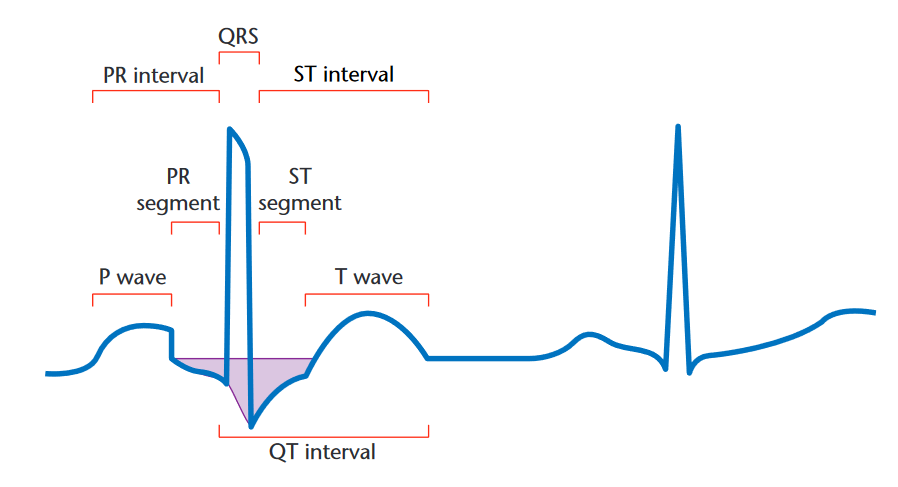
\includegraphics[width=0.75\textwidth]{ecg.png}
	\caption{\citet{b_ecg} "ECG morphology recorded 
		in a lead facing the left ventricular free
		wall showing the different waves and
		intervals. Shading, atrial repolarization
		wave."}
	\label{figure:ecg}
\end{figure}

\begin{figure}[!h]
	\centering
	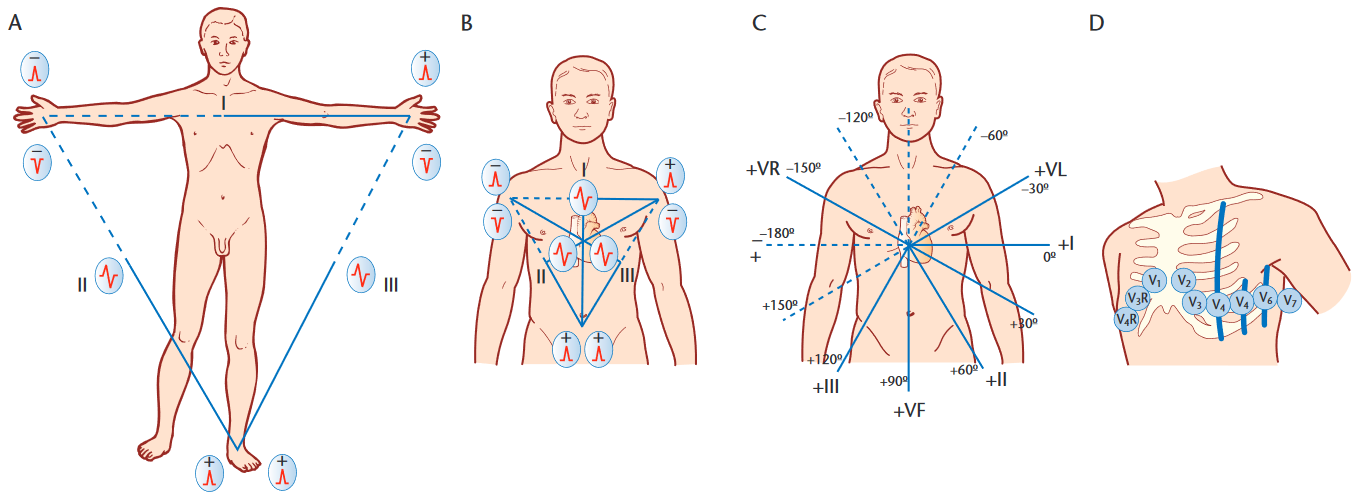
\includegraphics[width=0.90\textwidth]{ecg_leads.png}
	\caption{\citet{b_ecg} 
		"(A) Einthoven’s triangle. (B) Einthoven’s triangle superimposed on a human thorax. Note the positive (continuous line) and
		negative (dotted line) part of each lead. (C) Bailey’s hexaxial system. (D) Sites where positive poles of the six precordial leads are located."}
	\label{figure:ecg_leads}
\end{figure}

The test conditions of the system required the ECG signal to be processed in order to estimate the \ac{hr}. As described in \cref{chapter:Data Processing} this processing had to be made in two different situations, in real-time with limited computational resources and off-line without any computational restrictions and with maximum precision.

For the first situation the method proposed by \citet{segmenter} served as a base to build the used algorithm. Although the publication having several years, the method it proposes fulfills all the requirements the test conditions required. Being based on amplitude thresholding it runs in O(N) \cite{big_o} with very few calculations needed. In the literature it is possible to find similar algorithms to the one proposed, as in \citet{b_segmenter, b_segmenter_2, b_segmenter_3} with several more summarized in \citet{b_segmenter_revisiting}. Although these algorithms may perform slightly better, they still require much more computations over the entire length of the signal window, making them less fitted for the intended application.
%As the intended value to calculate was an approximation of the \ac{hr} over each 10s window, instantaneous \ac{hr} was not relevant and some error was admissible, allowing for the choice of the simplest algorithm.

\citet{b_segmenter} summarizes the most popular algorithms to process the \ac{qrs} and tries to determine which is the best one to process finger-based ECG, proposing a novel algorithm that is put against all others it mentions. The proposed algorithm is a real-time and very simple set of rules based on amplitude thresholding, similar to the one utilized in the present work.

In the algorithm proposed by \citet{b_segmenter_2}, several analog and digital filtering stages were implemented including bandpass and notch filters. The detection itself is made using and a convolution operation with a template QRS complex. Again, this approach presented a computational overhead t large to be feasible.

For the off-line \ac{hr} calculation, where precision was a requisite, and there were no limitations on calculation time and resources, the algorithm proposed by \citet{engzee} was the one chosen. This is a well established algorithm and although many more were proposed to do the same thing  e.g. the one by \citet{b_segmenter_revisiting}, this one remains a good choice for processing ECG signal as it was one of best rated algorithms in the comparison made by \citet{b_segmenter_engzee_comparison}.

In the present work, the \ac{ecg} sensor used was BITalino. It is a very customizable sensor platform with high quality \ac{ecg} signal as demonstrated by \citet{bitalinobatista2017experimental} and \citet{bitalinoguerreiro2013bitalino}. It is very convenient as it is a commercial product already including \ac{bt} communication.

There are many possible variations in ECG acquisition setups regarding the number of electrodes (leads) and the type of these electrodes. According with \citet{b_ecg_sensor}, there are four main types of electrodes: dry, gelled, insulated and non-contact. This aspect influences the quality of the signal, resistance to noise introduction and motion artifacts, but most of all the choice of electrodes has major design implications. Although gelled electrodes ensure the best power transfer to the sensor, they tend to be glued to the skin with some kind of adhesive. Although this is suitable for short term acquisitions, it can become a source of discomfort for long-term acquisitions and is not suitable for wearable inclusion. Regarding the dry and insulated electrodes, they are usually not adherent to the skin, making them suitable for long-term acquisitions or where ease in placing and removing the electrodes is desired. Finally the non-contact electrodes provide the most versatile range of applications and can even be placed over cloth.

In \citet{b_ecg_sensor2} an ECG sensor embedded in a t-shirt with insulated electrodes is presented, illustrating the easy integration of this sensors in the daily life of the person being monitored. This may present a major advantage regarding the adoption of systems based on this type of sensor.

Another approach is to embedd dry electrodes in a chest band. This is a popular method and was utilized by \citet{b_ecg_sensor3} in a very similar manner as in the present work. Dry electrodes are placed in a chest band with BT connectivity, sending data to a central monitor.



\FloatBarrier
\section{PPG}

\ac{ppg} acquisition is a way of estimating the \ac{bvp}, that can be used, among other, to determine the HR and, in certain conditions, the blood oxygen saturation as explained by \citet{b_ppg}. For oximetry, two \ac{led} of different wavelength are necessary, whereas for HR determination a single \ac{led} is enough.

Traditionally \ac{ppg} devices were placed in the fingers or ear lobes, however, in recent years, with the advent of wearables and smartwaches, there are many devices with wrist-worn \ac{ppg} sensors and other locations as presented by \citet{b_ppg_revisao}. Although many locations for the sensors have been proposed, wrist-worn sensors are the ones that present less inconveniences and are less prone to disturb daily life activities, as it is desired for pervasive monitoring.

There are authors that have built and designed their own custom hardware with many variations to perform PPG measurement. As an example, \citet{b_ppg_sensor} describes a wrist band designed to collect several bio-signals, including PPG used for HR determination. In addition, many commercially available products nowadays, include this type of sensor to appeal to customers who want to monitor themselves during daily life or even specifically during sports activities. This devices are evermore common and, some of them, have a good HR estimation capability as described by \citet{b_ppg_revisao2}.


Despite great potential, wearables have some drawbacks that greatly affect their usability. 
Smart- waches, in particular, position the PPG sensor in the distal portion of the posterior forearm. According with \citet{bvplee2016effective}, this is a location where PPG signal is faint due to reduced concentration of blood flow. Another major problem is signal corruption by motion artifacts as these devices tend to be heavy enough to have their own dynamics i.e. they move independently from the forearm by inertia. In addition, it is not comfortable to have the device too tight to the skin, and excessive pressure reduces superficial blood flow, thus further reducing \ac{snr}. In fact smartwaches and wearable sensors have been studied many times, for example by \citet{wearables} or \citet{sensor} and even its applicability as a source of clinical information has been proposed by some authors like \citet{compare, relogioarritmia} and \citet{doenca2}. However, the accuracy of this type of devices has been questioned and error margins for HR estimates produced by smartwaches were proven considerable for some devices by authors like \citet{compare, outroswearables} or \citet{compare2}.


As presented by \citet{b_ppg_revisao}, the use of green LEDs in PPG sensors is an evermore popular tendency and is the case of the sensor utilized in the currently proposed system. However this wavelength is not the ideal for this task as it is absorbed by tissues in a greater proportion than other wavelengths, making it capable of measuring only superficial blood flow. Despite the grater absorption of green light, this wavelength is, in fact, one of the the most absorbed by oxyhaemoglobin and deoxyhaemoglobin when compared to the usual red and infrared wavelengths, so it is possible to obtain better SNR although at shorter depths.

\begin{figure}[!h]
	\centering
	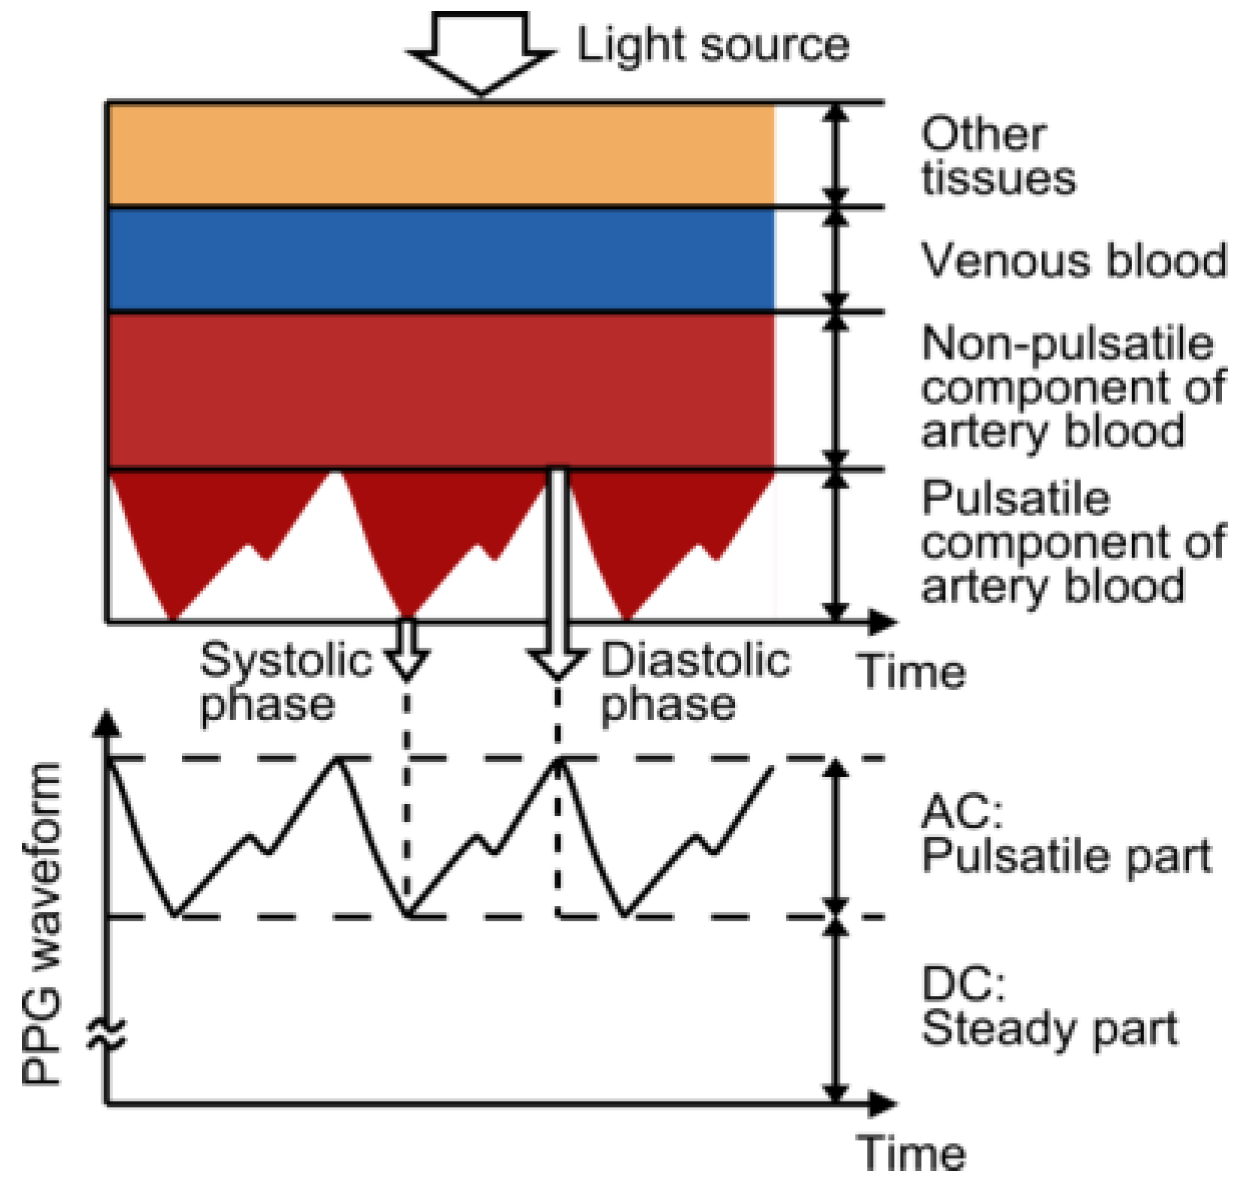
\includegraphics[width=0.6\textwidth]{ppg.png}
	\caption{\citet{b_ppg_revisao} 
		"Variation in light attenuation by tissue."}
	\label{figure:ppg}
\end{figure}

\begin{figure}[!h]
	\centering
	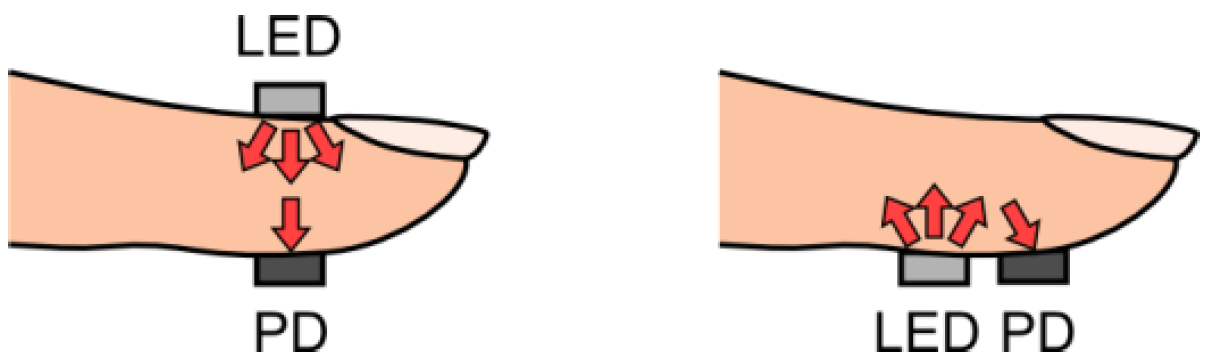
\includegraphics[width=0.8\textwidth]{ppg2.png}
	\caption{\citet{b_ppg_revisao} 
		" Light-emitting diode (LED) and photodetector (PD) placement for transmission- and reflectance-mode photoplethysmography (PPG)."}
	\label{figure:ppg2}
\end{figure}

As depicted in \cref{figure:ppg2}, there are two main types of PPG sensor, detecting transmitted and reflected light. Each of these types of sensors has their own set of positive and negative aspects. Transmission sensors have placing limitations, as not every part of the body is suitable for light to be transmitted in a practical way. This limitation makes reflection sensors the appropriate ones for wearable devices. However, reflection sensors are more sensitive to noise, as motion artifacts, mainly, can ruin the signal. To deal with this difficulty several algorithmic approaches have been developed.

As motion artifacts are one of the most prominent noise sources, most algorithm are designed to address it specifically, and not random noise like in other applications.

The simplest approach to PPG signal processing is the detection of signal features like the systolic peak, onset or others. This type of approaches were compared by \citet{bvponsetblazek2010multi} and evaluated on the performance in detecting onset, systolic peak or dicrotic notch of the PPG signal. Although this is, theoretically, enough to determine the HR from the PPG signal, in practice, this methods are very prone to error when noise is present in the signal. As this family of methods highly depends on the morphology of the signal, with the introduction of noise and motion artifacts the detection error increases very fast.

One of the most common approaches to motion artifact removal is adaptive filtering, as described by \citet{b_ppg_revisao}. There are many techniques based on this principle, that most frequently sets on the assumption of interference between the measured PPG signal and accelerations, usually measured with an accelerometer positioned in the same device as the PPG sensor. This interference can be modeled in many different ways, but most authors describe it as being a linear combination, many times simply additive i.e. the captured PPG signal is a linear combination of the true PPG signal and  a linear transformation of acceleration. This was the model used by \citet{laguerrewood2006active} to decorrelate ACC signal from the acquired PPG signal. In addition, the authors included one step of representing the signal with Laguerre coefficients before applying the adaptive filtering, this allows for a reduction of dimensionality, thus, decreasing the computational burden of the algorithm, while increasing its performance.

A different approach used by \citet{zhang2015joss} and \citet{zhang2015troika} is to look to the spectrum of the signal and reconstruct it using carefully chosen \ac{fft} segments. This works well even when there is in-band ACC noise i.e. when the spectral power of the motion artifacts is non-neglectable in the same regions as the relevant bandwidth PPG signal components.


%\bigskip
%\textcolor{red}{\Large \textbf{Reescrever}}
%\bigskip
%
%Due to poor quality PPG signal acquired, several algorithms were used in an attempt to get better HR estimates.
%Algorithms used included adaptive filtering with and without Laguerre expansion \cite{adagibbs2005active,laguerrewood2006active}, signal separation by sparse signal reconstruction \cite{zhang2015joss,zhang2015troika} and onset detection \cite{bvponsetblazek2010multi}. A total of 8 algorithms were used to process the PPG and accelerometry data coming from S3 to produce estimates of HR. However, the results obtained using all this algorithms performed equally bad, or even worse, than Gear's algorithm and for this reason, they were not mentioned previously. This clearly indicates that elevated error in Gear's HR estimations is probably related with a low quality signal and not with a poorly performing algorithm.
%
%\bigskip
%\textcolor{red}{\Large \textbf{------------------}}
%\bigskip

%\subsection{ACC  Processing}
%
%\bigskip
%\textcolor{red}{\Large \textbf{ACC}}
%\bigskip

\section{Physical activity}

Physical activity estimation can be useful in a variety of scenarios, from sports performance tracking, to patient recovery monitoring. Although a method to take this measurement may, intuitively, not be obvious, there are a few different ways of doing so. The main methods used are questionnaires, GPS monitoring and the extraction of indicators from \ac{acc} signals. All of them have downsides, and may not be suitable to cover all situations. Intuitively it is easy to understand that self-reported physical activity level is very prone to error. On the other hand GPS quantification is only suitable for activities implying great dislocations, as the GPS is not suitable for exercises in a gym environment for example. Finally accelerometry has a considerable disadvantage as the location of the sensors on the body conditions the type of activities it can successfully record, and most type having a full body monitoring is not practical nor possible.


\ac{acc} sensors are used to measure the acceleration they are subjected to, and when incorporated into a wearable device they can be used to detect movements and even estimate the physical activity level of the wearer as it was made by \citet{b_acc}. In this study, the purpose was to quantify the physical activity for different age groups. For this, subjects were asked to wear the measuring devices for 7 days and quantification was made using \ac{mets}. This is a popular way to quantify physical activity and it can be calculated from \ac{acc} data as defined by \citet{crouter_METS}.

Another approach to the physical activity analysis is trying to identify the activity being performed, in spite of trying to quantify its intensity. Many authors proposed methods for doing this type of activity recognition. \citet{b_acc2} presented a review of current methods for accomplishing this task. Methods are usually divided into similar stages with the collection of data, that is preprocessed, and then fed into some type of classifier producing the identification. Alongside algorithms to process ACC data, also video capture is a popular approach, although, only suitable for studying subjects in controlled environments, as opposed to daily life monitoring. 

\section{Data compression}

Regarding data compression for storing and relaying, some requirements were established, mainly related with performance and complexity of algorithms. Concerning the computational burden, the algorithms used had to be as simple and efficient as possible to reduce resource expenditure whereas for the algorithms themselves, they had to be lossless and it should be possible to compress segments of the signal, instead of having an algorithm compress the whole data.

There are many types of data compression algorithms, and the majority exploits some statistical property to find a smaller representation of the data. Although some algorithms are built to deal with a particular format of data, as the ones in \citet{b_ecg_compression} and \citet{b_ecg_compression_2} for example. However to maintain the versatility of the proposed system, the chosen algorithms to perform this task must be completely general on the signals to be compressed. For this reason, all data is seen as text strings, and like so, when compressing them as text, no data is lost and statistical properties become clearer when compared with numerical ones i.e. to represent numbers as strings only 12 symbols are needed (0-9, "-" and ".") eliminating the need to cover the range of each signal's value. At the same time, memory is limited and data size is relatively small, further limiting algorithm choice.

In \citet{b_textcompression} many algorithms are presented to perform data compression. However when taking into account the required utmost simplicity, Huffman static codding and time differencing were the chosen alternative.

%\bigskip
%\textcolor{red}{\Large \textbf{activity recognitin}}
%\bigskip

%%%%%%%%%%%%%%%%%%%%%%%%%%%%%%%%%%%%%%%%%%%%%%%%%%%%%%%%%%%%%%%%%%%%%%%%
%\section{Signal Processing}
%\label{section:theory1}
%
%\subsection{ECG Processing}
%
%
%\begin{figure}[!h]
%	\centering
%	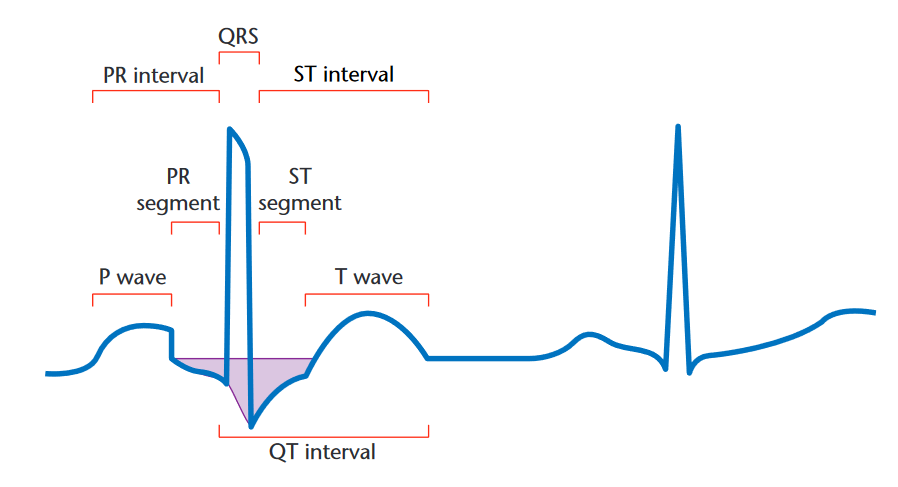
\includegraphics[width=0.85\textwidth]{ecg.png}
%	\caption{\citet{b_ecg} "ECG morphology recorded 
%		in a lead facing the left ventricular free
%		wall showing the different waves and
%		intervals. Shading, atrial repolarization
%		wave."}
%	\label{figure:ecg}
%\end{figure}
%
%\begin{figure}[!h]
%	\centering
%	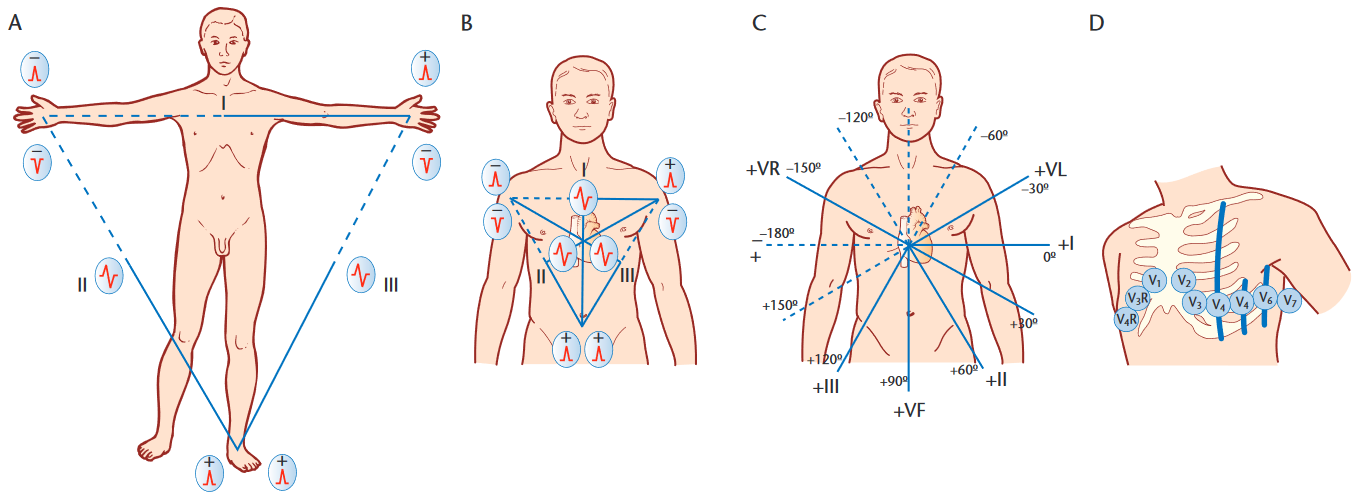
\includegraphics[width=0.90\textwidth]{ecg_leads.png}
%	\caption{\citet{b_ecg} 
%		"(A) Einthoven’s triangle. (B) Einthoven’s triangle superimposed on a human thorax. Note the positive (continuous line) and
%		negative (dotted line) part of each lead. (C) Bailey’s hexaxial system. (D) Sites where positive poles of the six precordial le
%		ads are located."}
%	\label{figure:ecg_leads}
%\end{figure}
%
%ECG is the recorded electrical activity of the heart muscle. This recording can be made with electrodes in a variety of standardized positions within the body as depicted in \cref{figure:ecg_leads}. Each electrode location will reflect in different signal morphologies that may contain different information. The mos commonly viewed morphology is depicted in \cref{figure:ecg}.
%
%The test conditions of the system required the ECG signal to be processed in order to estimate the \ac{hr}. As described in \cref{chapter:Data Processing} this processing had to be made in two different situations, in real-time with limited computational resources and off-line with no restrictions and with maximum precision.
%
%For the first situation the method proposed by \citet{segmenter} served as a base to build the used algorithm. Although the publication having several years, the method it proposes fulfills all the requirements the test conditions required. Being based on amplitude thresholding it runs in O(N) with very few calculations needed \cite{big_o}. In the literature it is possible to find similar algorithms to the one proposed, as in \citet{b_segmenter, b_segmenter_2, b_segmenter_3} with several more summarized in \citet{b_segmenter_revisiting}. Although these algorithms may perform slightly better, they still require much more computations over the entire length of the signal window.
%%As the intended value to calculate was an approximation of the \ac{hr} over each 10s window, instantaneous \ac{hr} was not relevant and some error was admissible, allowing for the choice of the simplest algorithm.
%
%\citet{b_segmenter} summarizes the most popular algorithms to process the \ac{qrs} and tries to determine what is the best to process finger-based ECG, and also proposing another algorithm. The proposed algorithm is a real-time and very simple set of rules based on amplitude thresholding, similar to the one utilized in the present work.
%
%In the algorithm proposed by \citet{b_segmenter_2}, several analog and digital filtering stages were implemented including bandpass and notch filters. The detection itself is made using and a convolution operation with a template QRS complex.
%
%For the off-line \ac{hr} calculation, where precision was a requisite, and there were no limitations os calculation time and resources, the algorithm proposed in \citet{engzee} was the one chosen. This is a well established algorithm and although many more were proposed to do the same thing \citet{b_segmenter_revisiting}, this one remains a good choice for processing ECG signal as it was one of best rated algorithms in the comparison made by \citet{b_segmenter_engzee_comparison}.



%\subsection{PPG Processing}
%
%As presented by \citet{b_ppg_revisao}, the use of green LEDs in PPG sensors is an evermore popular tendency and is the case of the sensor utilized in the currently proposed system. However this wavelength is not the ideal for this task as it is absorbed by tissues in a greater proportion than other wavelengths, making it capable of measuring only superficial blood flow. Despite the grater absorption of green light, this wavelength is, in fact, one of the the most absorbed by oxyhaemoglobin and deoxyhaemoglobin compared to infrared light, so it is possible to obtain better SNR although at shorter depths.
%
%\begin{figure}[!h]
%	\centering
%	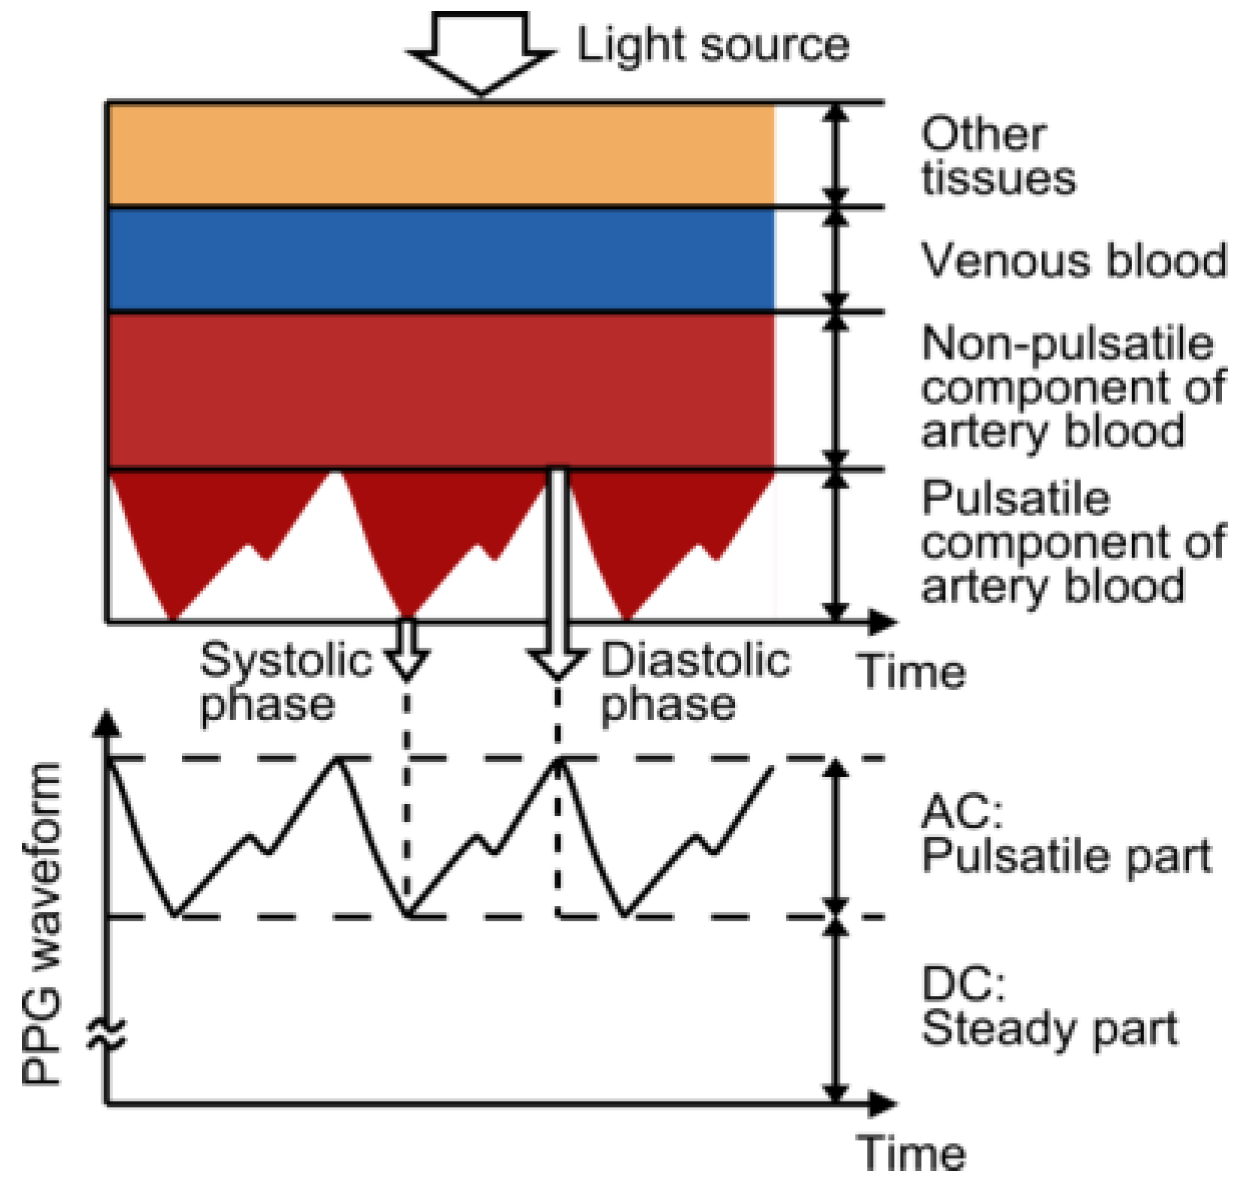
\includegraphics[width=0.90\textwidth]{ppg.png}
%	\caption{\citet{b_ppg_revisao} 
%		"Variation in light attenuation by tissue."}
%	\label{figure:ppg}
%\end{figure}
%
%\begin{figure}[!h]
%	\centering
%	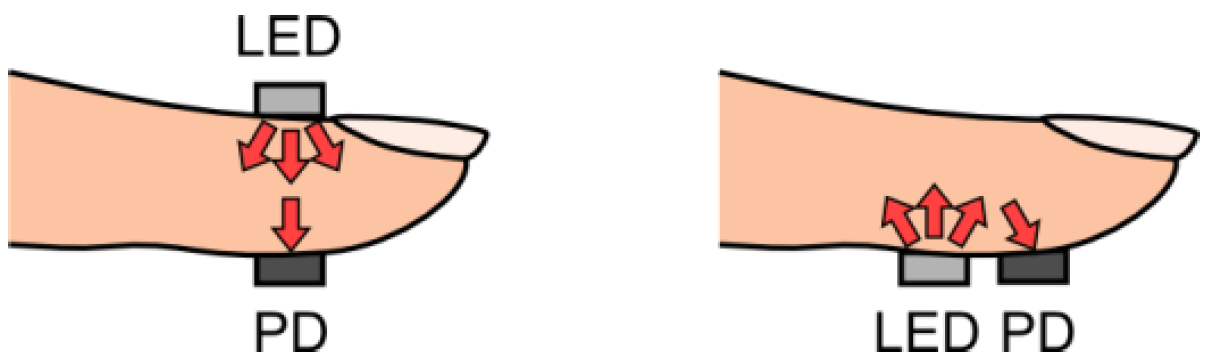
\includegraphics[width=0.90\textwidth]{ppg2.png}
%	\caption{\citet{b_ppg_revisao} 
%		" Light-emitting diode (LED) and photodetector (PD) placement for transmission- and reflectance-mode photoplethysmography (PPG)."}
%	\label{figure:ppg}
%\end{figure}
%
%\bigskip
%\textcolor{red}{\Large \textbf{Reescrever}}
%\bigskip
%
%Due to poor quality PPG signal acquired, several algorithms were used in an attempt to get better HR estimates.
%Algorithms used included adaptive filtering with and without Laguerre expansion \cite{adagibbs2005active,laguerrewood2006active}, signal separation by sparse signal reconstruction \cite{zhang2015joss,zhang2015troika} and onset detection \cite{bvponsetblazek2010multi}. A total of 8 algorithms were used to process the PPG and accelerometry data coming from S3 to produce estimates of HR. However, the results obtained using all this algorithms performed equally bad, or even worse, than Gear's algorithm and for this reason, they were not mentioned previously. This clearly indicates that elevated error in Gear's HR estimations is probably related with a low quality signal and not with a poorly performing algorithm.
%
%\bigskip
%\textcolor{red}{\Large \textbf{------------------}}
%\bigskip
%
%%\subsection{ACC  Processing}
%%
%%\bigskip
%%\textcolor{red}{\Large \textbf{ACC}}
%%\bigskip



%\begin{itemize}
%  \item Citation mode \#1 - \quad \cite{telemold}
%  \item Citation mode \#2 - \quad \citet{telemold}
%  \item Citation mode \#3 - \quad \citep{telemold}
%  \item Citation mode \#4 - \quad \citet*{telemold}
%  \item Citation mode \#5 - \quad \citep*{telemold}
%  \item Citation mode \#6 - \quad \citealt{telemold}
%  \item Citation mode \#7 - \quad \citealp{telemold}
%  \item Citation mode \#8 - \quad \citeauthor{telemold}
%  \item Citation mode \#9 - \quad \citeyear{telemold}
%  \item Citation mode \#10 - \quad \citeyearpar{telemold}
%\end{itemize}



 % file "Thesis_Background.tex"
\cleardoublepage


\chapter{System Description}
\label{chapter:description}

\section{Overview}

The implemented data acquisition system was designed to collect medically relevant data and display it in real time through a web interface. This allows medical teams to permanently monitor patients and access patient's information remotely, including real time data and also the history of past values, allowing to detect patterns associated with certain diseases and monitor the progression or even check medication effectiveness.
Being completely mobile the system allows for a constant monitoring of hospitalized and non-hospitalized patients for periods that can go up to two months without the need for any maintenance, except for charging devices' battery obviously.
The system in prepared to deal with any numerical variables that can be collected with any sensor that has a \ac{bt} interface. This makes for a versatile completely in what sensors it can interact with and, thus what variables it can acquire, which make it suitable for almost all situations where pervasive long term monitoring can be useful.

Incoming data from sensors is collected into a smartphone that sends it, via web, to a central server that stores the data and serves the web interface. Physicians can specify which sensors should be active with each patient and which are the relevant variables to be acquired and displayed.

\begin{figure}[!h]
	\centering
	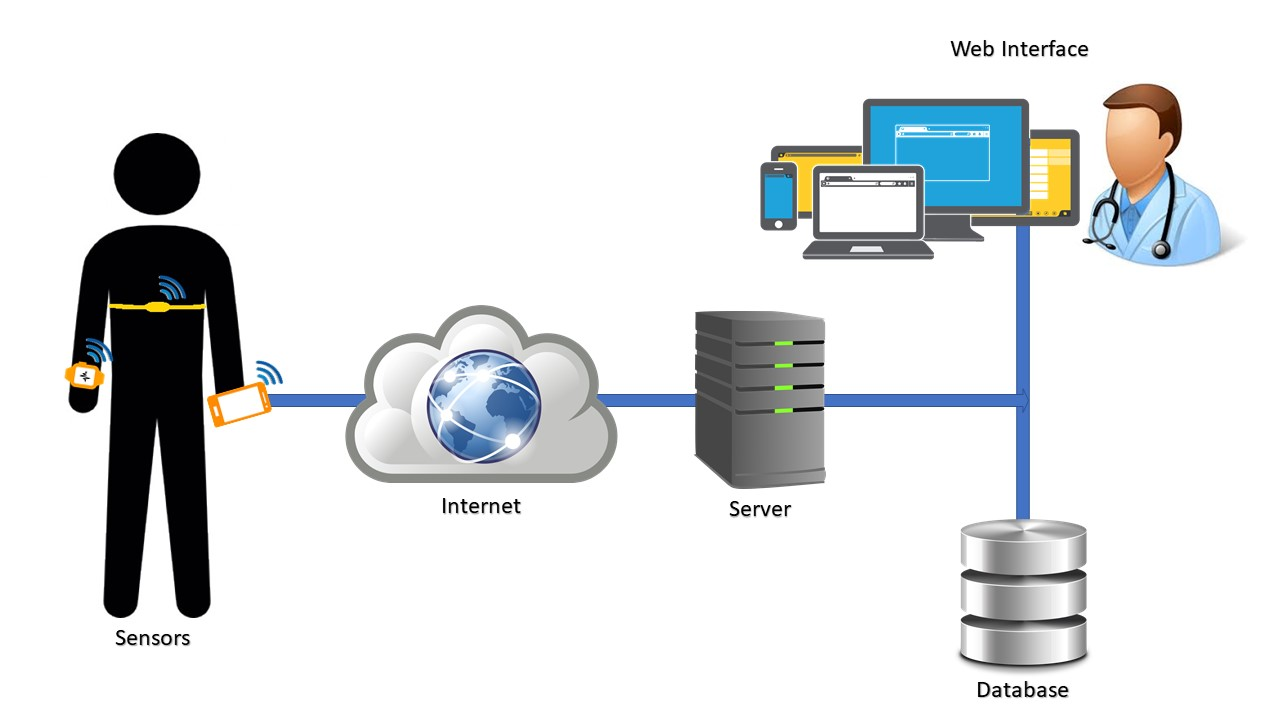
\includegraphics[width=\textwidth]{overview.jpg}
	\caption{System's architecture. Bluetooth connectivity between wearable devices. Smartphone connects to server through mobile web connection.}
	\label{fig:overview}
\end{figure}



The system works by having a physician configure all the acquisition parameters relevant for a certain patient and after this step no further intervention is needed, apart from equipping the patient and turning devices on. Parameters that can be configured are:
\begin{itemize}
	\item The type of devices currently available in the system (smartphone, smartwaches, etc...)
	\item What devices are to be given to the patient;
	\item What variables are to be collected from each device, and with what frequency they should be sent to the central server;
	\item The variables that are expected to be received by the server (that may not be the ones collected, some processing can occur) and how they should be visualized (color, range, etc...)
	\item Several alarms can be set defining what variable should be in what range for how long to trigger the alarm e.g. heart rate is below 50\ac{bpm} for more than 5 minutes;
\end{itemize}
This information is saved into the database. After the smartphone is turned on, information is retrieved from the server and acquisition starts. Until the end of the study data is continuously sent to the server where the physician can analyze it in real time (which is actually a 30s delay that is irrelevant for clinical practice.)

\begin{figure}[!h]
	\centering
	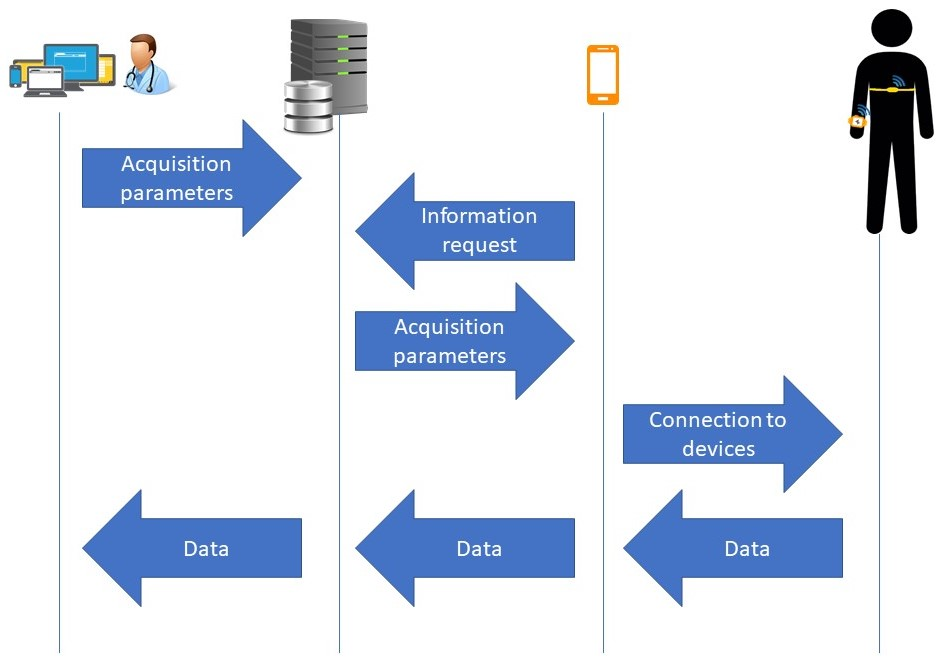
\includegraphics[width=\textwidth]{overview_info.jpg}
	\caption{System's data flow overview. Bluetooth connectivity between wearable devices. Smartphone connects to server through mobile web connection.}
	\label{fig:overview2}
\end{figure}

%Due to the multiplicity of devices used, several independent software components were developed to interact with each device and with the various sensors as illustrated in \cref{fig:platforms}.

\Cref{fig:overview} illustrates the general system architecture, where the local sensor network connects to a smartphone that relays information through web to a central server that manages the database and the web interface accessible to medical teams. \Cref{fig:overview2} depicts the timeline of communications between devices. Initially the user specifies the parameters in the interface that are stored in the database. When devices are turned on the smartphone pings the server which answers with the user configurations so it can start the communication with the configured sensors. After this the flow becomes mostly unidirectional with data coming from the sensors being relayed by the smartphone (eventually with some processing happening before) to the server then to saved into the database and displayed in the user interface when required.


%\FloatBarrier

\section{Devices}



\FloatBarrier
\subsection{Smartphone}

The smartphone is used to centralize data from the various sensors and as a local storage and processing unit. It receives all the raw data collected from the connected sensors, stores it into an \ac{sd} memory card, applies the necessary algorithms to extract information from the raw signals and finally sends this computed quantities to a central server so they can be visualized through a web interface.

All the sensors' data is transmitted through a Bluetooth interface and is stored as an array so it can be used to make the necessary calculations. Every 10s the data is saved into files stored in an \ac{sd} memory card. Data to be saved consists of time-series composed by consecutive data samples from the sensors. This samples are acquired at different rates from each sensor and a timestamp is associated to each sample in order to facilitate the time location of each one and make easier to align the signals from different sensors. The app is prepared to deal with any number of sensors per connected device and it stores data in a separate file for every remote device, containing data from all the device's sensors.


%\begin{figure}[!h]
%	\centering
%	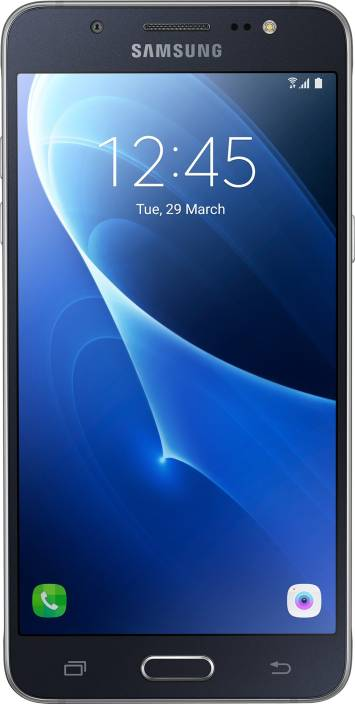
\includegraphics[width=0.2\textwidth]{samsung-j5.jpeg}
%	\caption{Smartphone Samsung J5}
%	\label{fig:phone}
%\end{figure}

\subsubsection{Android App}

The android app was implemented using Android Studio 3.0.1. All functions were designed to be as computationally efficient as possible to minimize time delay and maximize battery life. The app was designed as a replacement of the android home screen, so when the smartphone is turned on, the app will automatically initiate and show on screen, ensuring the patient does not forget to initiate it. Another focal point of the implemented app is the thread-oriented logic that eases future development and new sensors integration. This means that support and communication for each sensor runs in an independent thread, easing the process of introducing support for new remote sensors.

At startup, in the main thread, the app checks for Internet and Bluetooth connectivity, requesting its activation if necessary. A background service is initiated and it will be responsible for all the non-display actions. This was necessary not to crash the display as background tasks can be time consuming and will need to run even if the display is deactivated or if the screen is locked.
The background service then starts its task by establishing a socket \cite{tcpip} to the server @learnib.lx.it.pt and sending the smartphone's \ac{uuid} which is the Wi-Fi mac address. Initially the Bluettoth adapter address was to be used as \ac{uuid} for the smartphone, but recent versions of Android \ac{os} do not allow to programmatically get it so, alternatively, Wi-Fi mac address was used. 

\FloatBarrier

Code used to determine smartphone's mac address:

\bigskip
\begin{lstlisting}[language=Java]
import android.annotation.TargetApi;
import java.net.NetworkInterface;
import android.bluetooth.BluetoothAdapter;
import java.util.List;


@TargetApi(9)
public static String getMacAddr() {
	BluetoothAdapter bluetoothAdapter = BluetoothAdapter.getDefaultAdapter();
	if(bluetoothAdapter == null){
		return null;
	}	
	String addr = bluetoothAdapter.getAddress();	
	try {
		if (addr.equals("02:00:00:00:00:00")) {		
			List<NetworkInterface> all = Collections.list(NetworkInterface.getNetworkInterfaces());
			for (NetworkInterface nif : all) {
				if (!nif.getName().equalsIgnoreCase("wlan0")) continue;			
				byte[] macBytes = nif.getHardwareAddress();
				if (macBytes == null) {
					return "";
				}
				StringBuilder res1 = new StringBuilder();
				for (byte b : macBytes) {
					res1.append(String.format("%02x", b) + ":");
				}				
				if (res1.length() > 0) {
					res1.deleteCharAt(res1.length() - 1);
				}
				Log.d(TAG, "MAC ADRSS: " + res1.toString());
				return res1.toString();
			}
		}
	} catch (Exception ex) { }
	return addr;
}
\end{lstlisting}
\bigskip

Connection to the server is made using java's native socket implementation:

\bigskip
\begin{lstlisting}[language=Java]
import java.net.Socket;

private Socket socket;
private OutputStream out;
private InputStream in;
private final String host = "learnbig.lx.it.pt";
private final int port = ********;

public void connect() {
	try {
		socket = null;
		out = null;
		in = null;
		socket = new Socket();		
		socket.connect(new InetSocketAddress(this.host,this.port), 10000);
		out = socket.getOutputStream();
		in = socket.getInputStream();
	}
	catch (Exception e) {}
	catch (Throwable t) {}
}
\end{lstlisting}
\bigskip

After the socket is connected, the \ac{uuid} is sent to the server that replies with a message containing the Bluetooth mac addresses of all the remote devices and sensors that the smartphone should connect to. It also sends the information about the frequency at which data should be sent to the server and, if necessary, other device-specific parameters. In case of connection failure the background service sends this information using a previously registered ResultReceiver causing the \ac{ui} activity to change the background color and send a notification with sound to the user while simultaneously retrying to connect.

As this information is received and parsed, the necessary devices are initialized. A different class is implemented to interact with each type of device, as different communication protocols are required. Each of this classes extends the native Thread class in order to have complete independence between devices. This aspect enhances the versatility of the system, easing the implementation of support for new sensors. This is also needed to avoid clogging the processor and the Bluetooth reading buffers, as events occur asynchronously between devices and timing is relevant to ensure no data is lost.

\begin{figure}[!h]
	\centering
	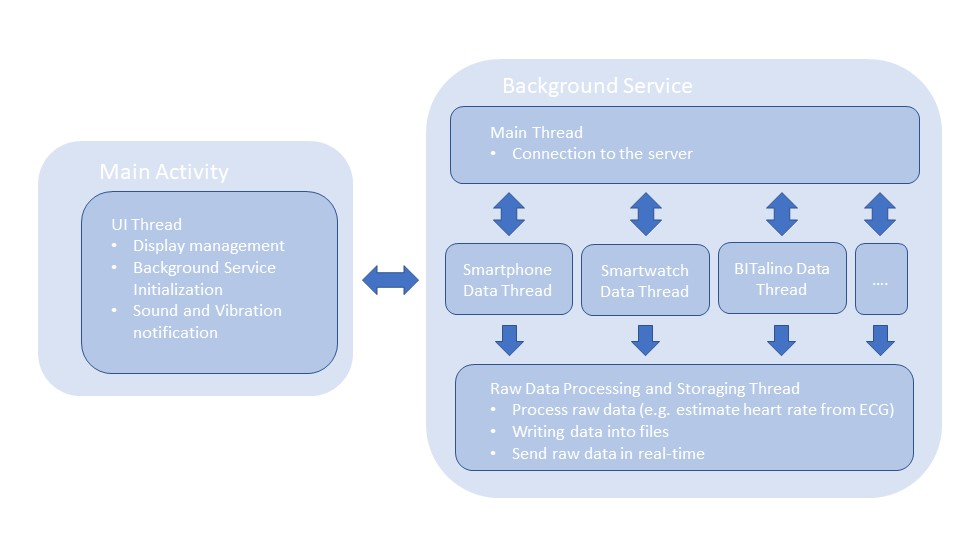
\includegraphics[width=\textwidth]{app_android.jpg}
	\caption{Android App threads call-stack}
	\label{fig:app_thread}
\end{figure}

Device's classes all work in similar ways. They establish a Bluetooth connection and handle the incoming data. As sensor values reach the smartphone, they are stored into buffers holding 10s of data. When buffers are full, the 10s window of data is compressed and saved into a file and the data is processed in order to extract medically relevant indicators like the \ac{hr} for example which are then displayed in the \ac{ui} thread. Saving data into the files is accomplished using BufferedWriter and StringBuilder classes for optimized performance \cite{android}. BufferedWriter class uses a non blocking write that allows the device thread to continue his strenuous work without much delay. StringBuilder class is used in order to compose the strings that ought to be saved without the need to allocate new memory blocks with each append as it would be necessary if dealing with Strings. Data is saved into an \ac{sd} card or to the smartphone memory if the early is not present. All file writing processes are synchronized to protect against a case where two threads are reading or writing to the same file at the same time.

\Cref{fig:app_thread} illustrates the general architecture of the implemented app, showing the two services with their threads. Background service, as refered before, has a main thread that establishes connection to the server, than a separate thread to interact with each device and finally a thread to save and process data. 


Data is saved to files in a specific format detailed in \cref{chapter:compresion} and the code utilized to save it most efficiently is as follows:

\bigskip
\begin{lstlisting}[language=Java]
import java.io.BufferedWriter;
import java.io.File;
import java.io.FileInputStream;
import java.io.FileNotFoundException;
import java.io.FileReader;
import java.io.FileWriter;
import java.io.IOException;
import java.nio.*;

private BufferedWriter bw = null;
private File file;

public open_file(Context ctx, String device, String person_ID) {

	context = ctx;
	this.person_ID = person_ID;
	File[] paths = context.getExternalFilesDirs(null);
	File path;
	int n = 0;
	
	if (paths.length == 2) {
		path = paths[1];
	} else {
		path = paths[0];
	}
	
	file = new File(path, device + "_" + person_ID + ".txt");
	
	try {
		bw = new BufferedWriter(new FileWriter(file, true));
	} catch (IOException e) {
		e.printStackTrace();
		Log.d(TAG, "Erro erro ao abrir o writer");
		try {
			file.createNewFile();
			bw = new BufferedWriter(new FileWriter(file, true));
		} catch (Exception ex) {
			Log.d(TAG, "Erro erro ao abrir o writer depois de criar o ficheiro");
			e.printStackTrace();
		}
	
	}
	
	Log.d(TAG, "Iniciou com sucesso");
}

public void insert_data_list(int[] RAWmeasurementsArray, Long[]  RAWtimestampsArray) {

	StringBuilder str = new StringBuilder();
	int buf = 0;
	Long buf_time = 0L;
	String separator = ";";
	
	str.append("#");
	str.append(separator);
	
	for (int i = 0; i < RAWmeasurementsArray.length; i++) {
		str.append(String.valueOf((Long) RAWtimestampsArray[i] - buf_time));
		buf_time = (Long) RAWtimestampsArray[i];	
		str.append(separator);
		str.append(String.valueOf(RAWmeasurementsArray[i] - buf));
		buf = RAWmeasurementsArray[i];
	}
	str.append("\n");
	
	synchronized (bw) {
	
		try {
			bw.write(str.toString());
		} catch (IOException e) {
			e.printStackTrace();
			Log.d(TAG, "Erro ao escrever ficheiro");
			try {
				bw[this.index] = new BufferedWriter(new FileWriter(files[this.index], true));
			} catch (IOException e1) {
				e1.printStackTrace();
				Log.d(TAG, "Erro ao abrir ficheiro");
			}
		}
	}
	
	str = new StringBuilder();
	
	try {
		bw.flush();
	} catch (IOException e) {
		e.printStackTrace();
		try {
			bw = new BufferedWriter(new FileWriter(file, true));
		} catch (IOException e1) {
			e1.printStackTrace();
		}
	}
}


\end{lstlisting}
\bigskip


Optionally, using the web interface, user can request raw data in real time from a specific or all devices to be sent. This process is accomplished by a separate thread that receives each 10s block of data that is written to files, further compresses and sends it through a socket to the server where data is stored.
Further compression is needed as bandwidth and internet plafond are more restrictive than memory space. Data compression and sending occurs in a separate thread to ensure there is no delay in data acquisition.

At the same time data is saved into files by each device's thread, the result of processing that 10s window of data is sent to the \ac{ui} thread to be displayed on screen. These threads also request battery status from the devices. This information is sent to the \ac{ui} thread where a symbol indicates battery status of each device.

To summarize, raw data coming from the sensors is stored into files and optionally sent to the server. That same data is then processed to extract more relevant and 
informative measures, that are again sent to the server and shown in the smartphone screen alongside with battery status and Bluetooth connection status. \Cref{fig:app} shows the main screens of the app with the main stages of initialization (\cref{fig:app1,fig:app2,fig:app3}) and when connection to the server cannot be made (\cref{fig:app4}).


\begin{figure}[!t]
	\centering
	\makebox[\linewidth][c]{%
		\begin{subfigure}[t]{0.5\textwidth}
			\centering
			\captionsetup{width=.75\linewidth}
			\fbox{
\includegraphics[width=0.6\textwidth]{screen_on.png}}
			\caption{Display at startup showing device's \ac{uuid}}
			\label{fig:app1}
		\end{subfigure}%
		\begin{subfigure}[t]{0.5\textwidth}
			\centering
			\captionsetup{width=.75\linewidth}
			\fbox{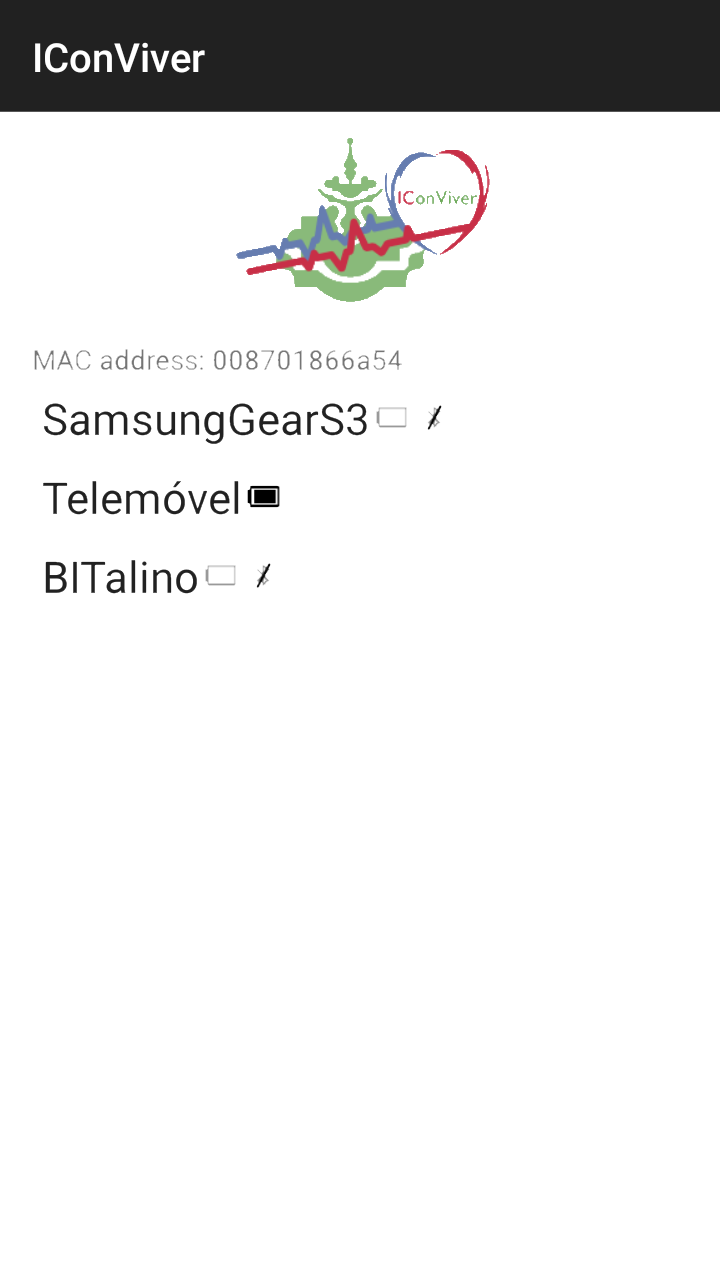
\includegraphics[width=0.6\textwidth]{screen_on1.png}}
			\caption{Display after information from the server is received. Bluetooth symbols indicate there is still no connection with peripheral devices.}
			\label{fig:app2}
		\end{subfigure}%
	}\\
	\makebox[\linewidth][c]{%
		\begin{subfigure}[t]{0.5\textwidth}
			\centering
			\captionsetup{width=.75\linewidth}
			\fbox{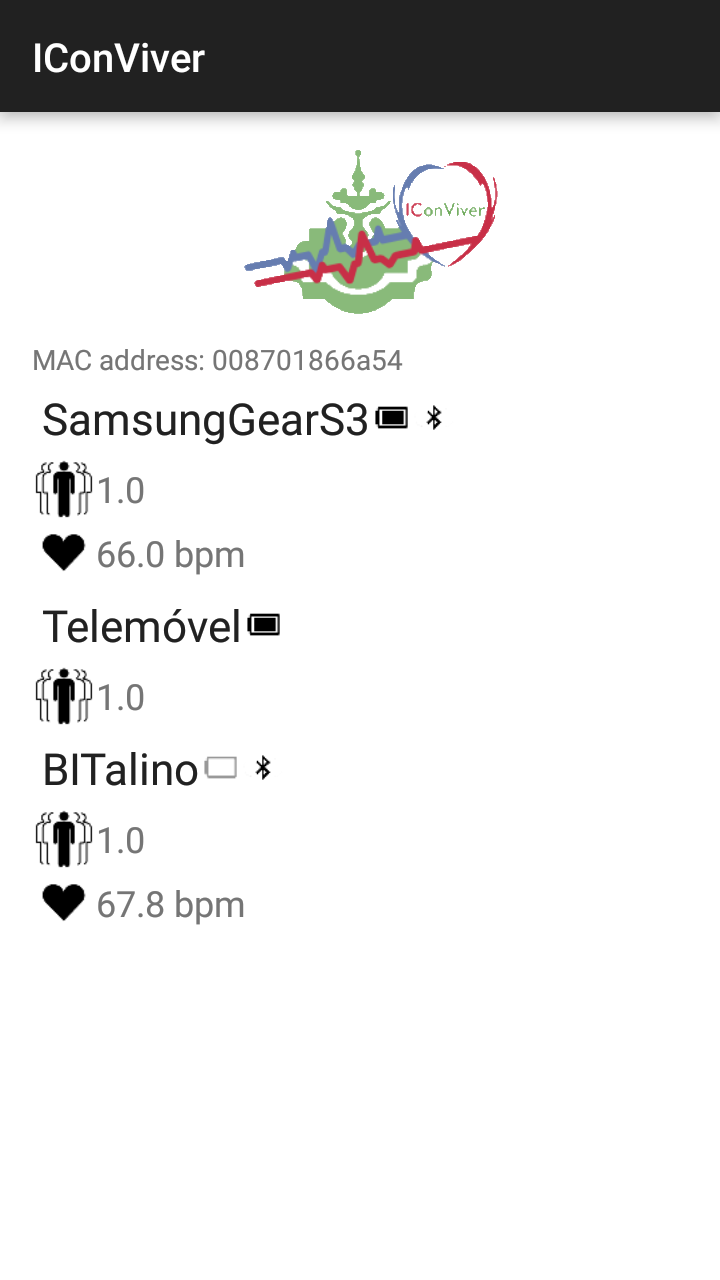
\includegraphics[width=0.6\textwidth]{screen_on2.png}}
			\caption{Display after connection has been established and data from devices is received. Below each device's name there is the value resulting from processing the last 10s of data collected.}
			\label{fig:app3}
		\end{subfigure}%
		\begin{subfigure}[t]{0.5\textwidth}
			\centering
			\captionsetup{width=.75\linewidth}
			\fbox{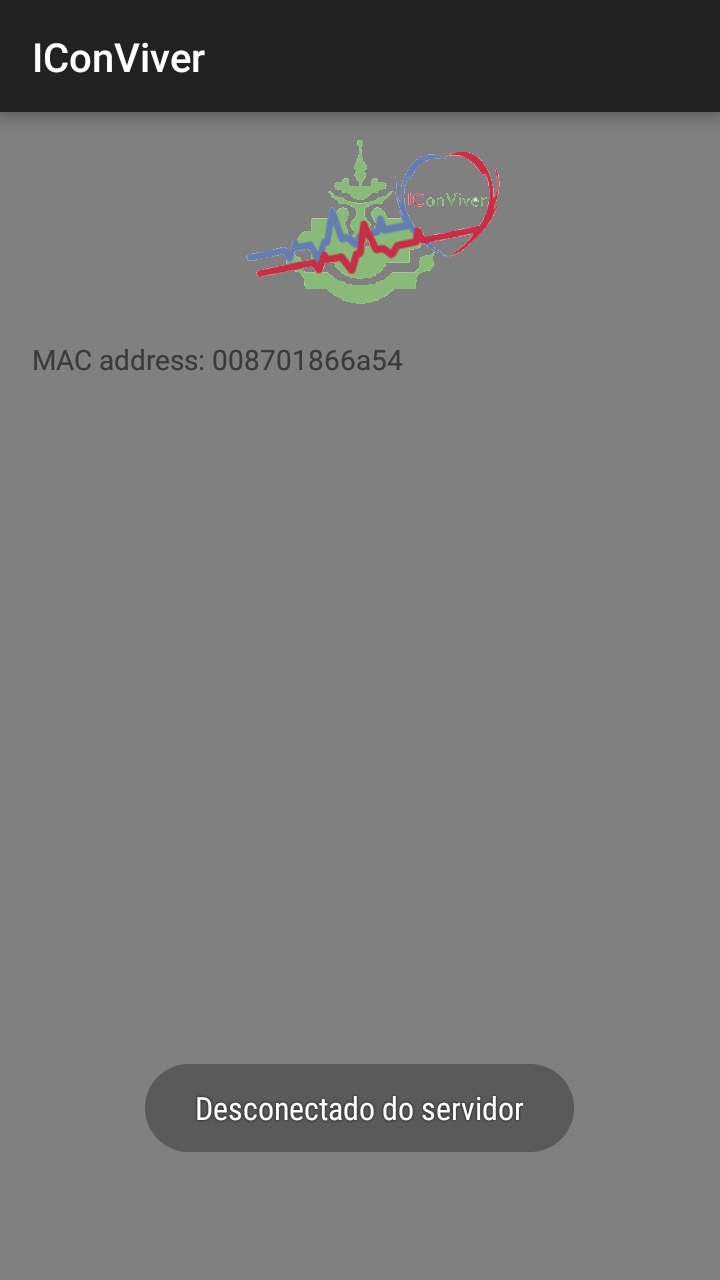
\includegraphics[width=0.6\textwidth]{screen_off.png}}
			\caption{Screen when it was not possible to establish server connection. A sound notification also occurs in this event.}
			\label{fig:app4}
		\end{subfigure}%
	}\\
	\caption{Android App screen in different situations.}
	\label{fig:app}
\end{figure}

In case any Bluetooth connection to any remote device is lost, the corresponding device's thread will try to reconnect it indefinitely and will trigger a notification with sound and an icon will appear in the app screen informing the user connection is lost. This is useful in case the user is not wearing one of the devices and forgets it. Also a warning message will be sent to the server and a mark will appear in data visualization, informing the medical teams of the momen the device was disconected. All threads and procedures will proceed normally when the lost connection is reestablished. In case the server connection is lost, background service's main thread will also try to reconnect indefinitely, leaving all other threads running with no interference. When reconnected, all other threads are stopped and the call-stack is restarted as if the app was just initialized. This occurs in this way to ensure that data acquisition continues even if the patient enters an area with no mobile data communication and, ant the same time, when the communication is reestablished, acquisition restarts to preclude any change in acquisition parameters. When the app cannot communicae with the server, or server is lost, a notification is emmited and the background color of the home screen changes.



\FloatBarrier

\subsection{Server and Web Interface}

\bigskip
\textcolor{red}{\Large \textbf{Pôr as figuras num anexo em vez de aqui no meio do texto?}}
\bigskip

\begin{figure}[h!]
	\centering
	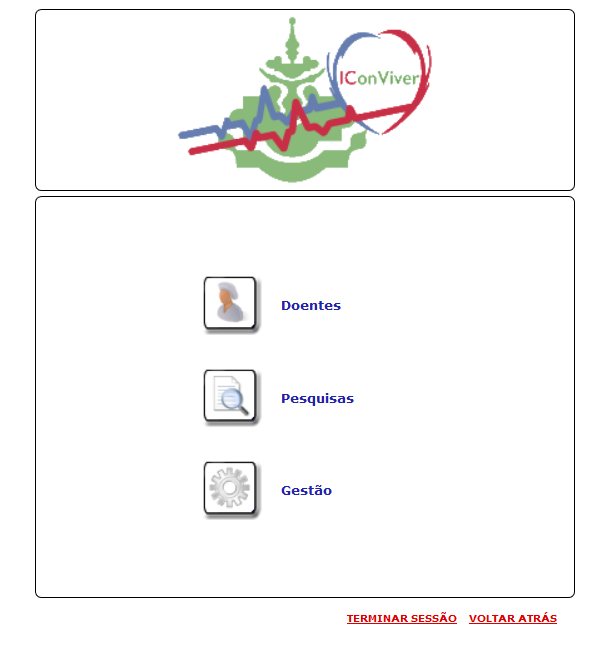
\includegraphics[width=0.45\textwidth]{login2.png}
	\captionsetup{width=0.4\textwidth}
	\caption{Initial panel after login into the system's web interface. Here one can see patient information; search for specific data of a particular patient; configure all device and acquisition parameters.}
	\label{figure:UI1}
	
\end{figure}%

\begin{figure}[h!]
	\centering
	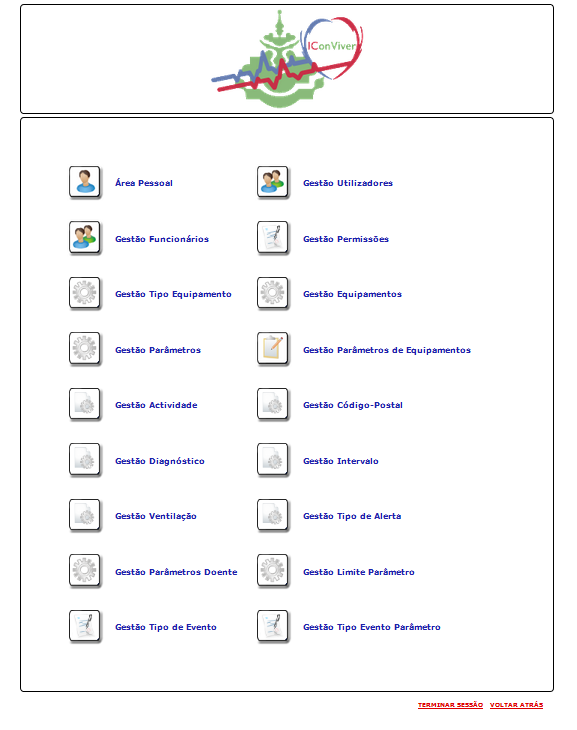
\includegraphics[width=0.85\textwidth]{gestao.png}
	\captionsetup{width=0.8\textwidth}
	\caption{Management screen, where all the systems and device's parameters can be defined.}
	\label{figure:UI_gestao}
	
\end{figure}%

\begin{figure}[h!]
	\centering
	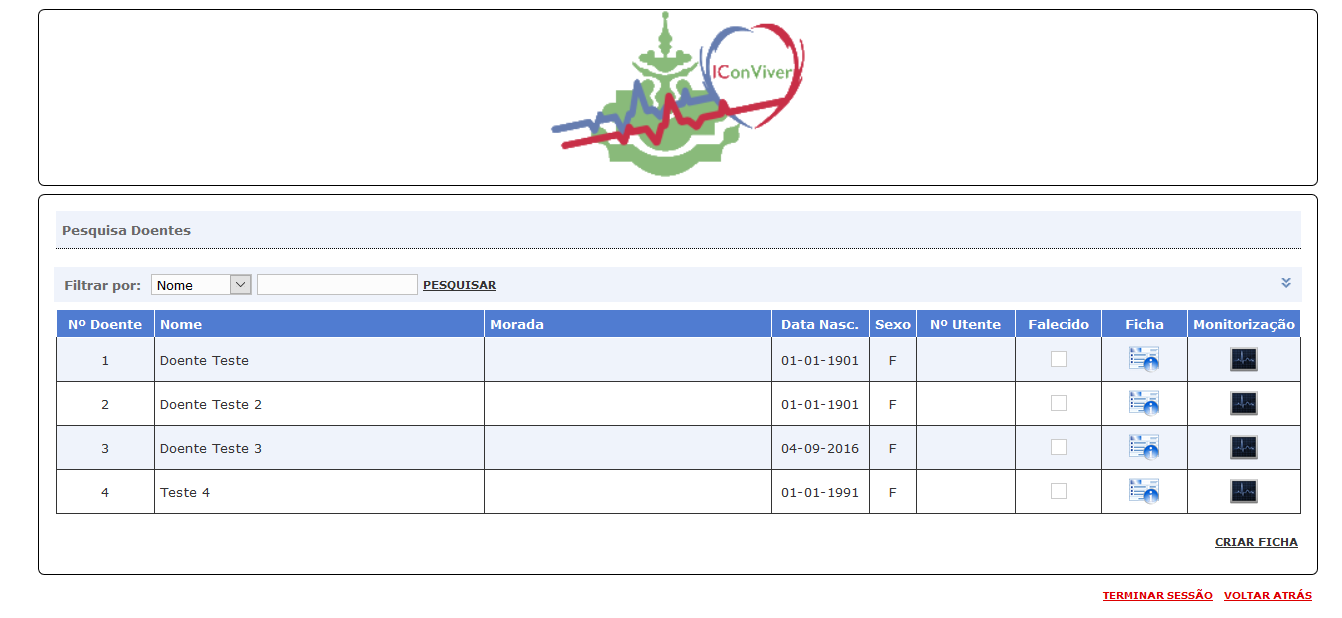
\includegraphics[width=0.85\textwidth]{doentes2.png}
	\captionsetup{width=0.8\textwidth}
	\caption{Screen showing the patients enrolled in the system. From here one can access all the information and collected data from each patient.}
	\label{figure:UI2}
\end{figure}%


\begin{figure}[h!]
	\centering
	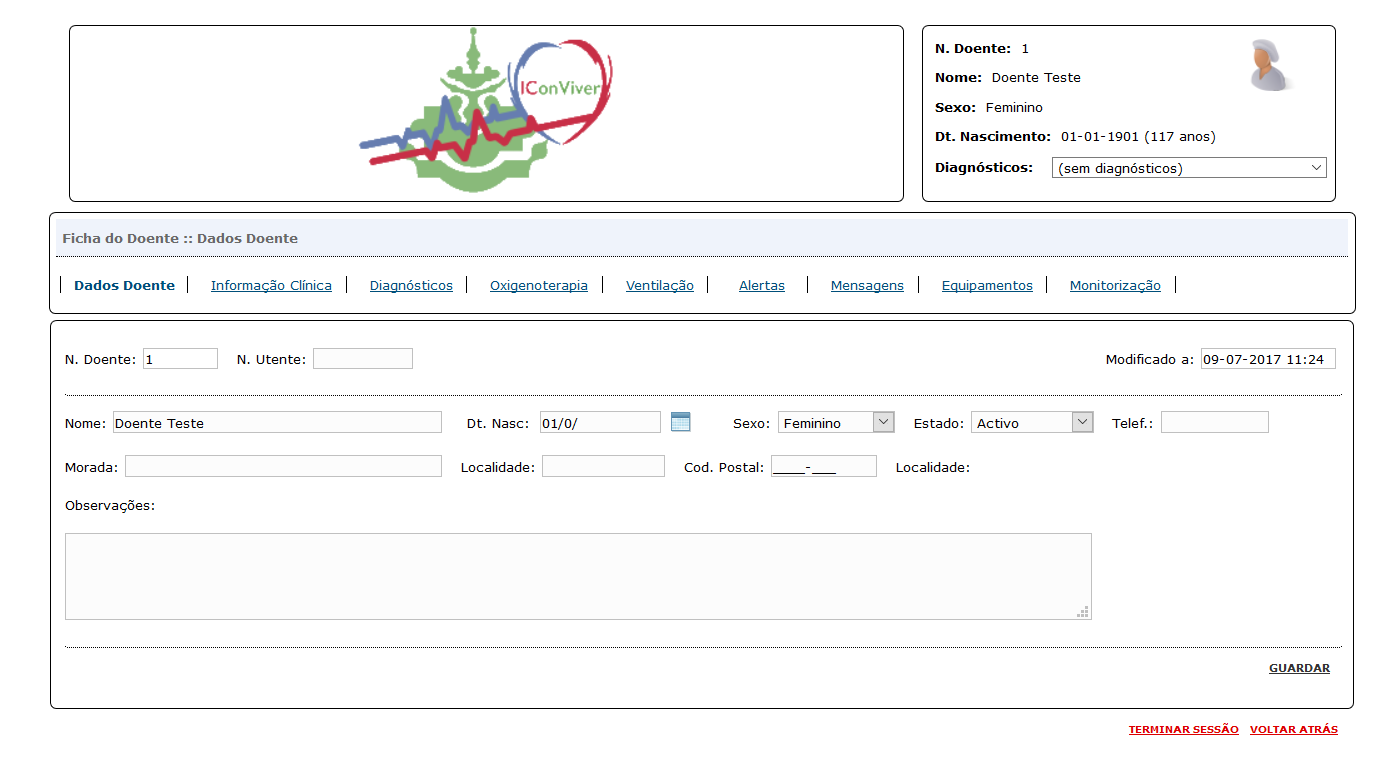
\includegraphics[width=0.85\textwidth]{paciente.png}
	\captionsetup{width=0.8\textwidth}
	\caption{Data visualization screen where one can choose the variables to see and their time frame.}
	\label{figure:UI4}
\end{figure}%

\begin{figure}[h!]
	\centering
	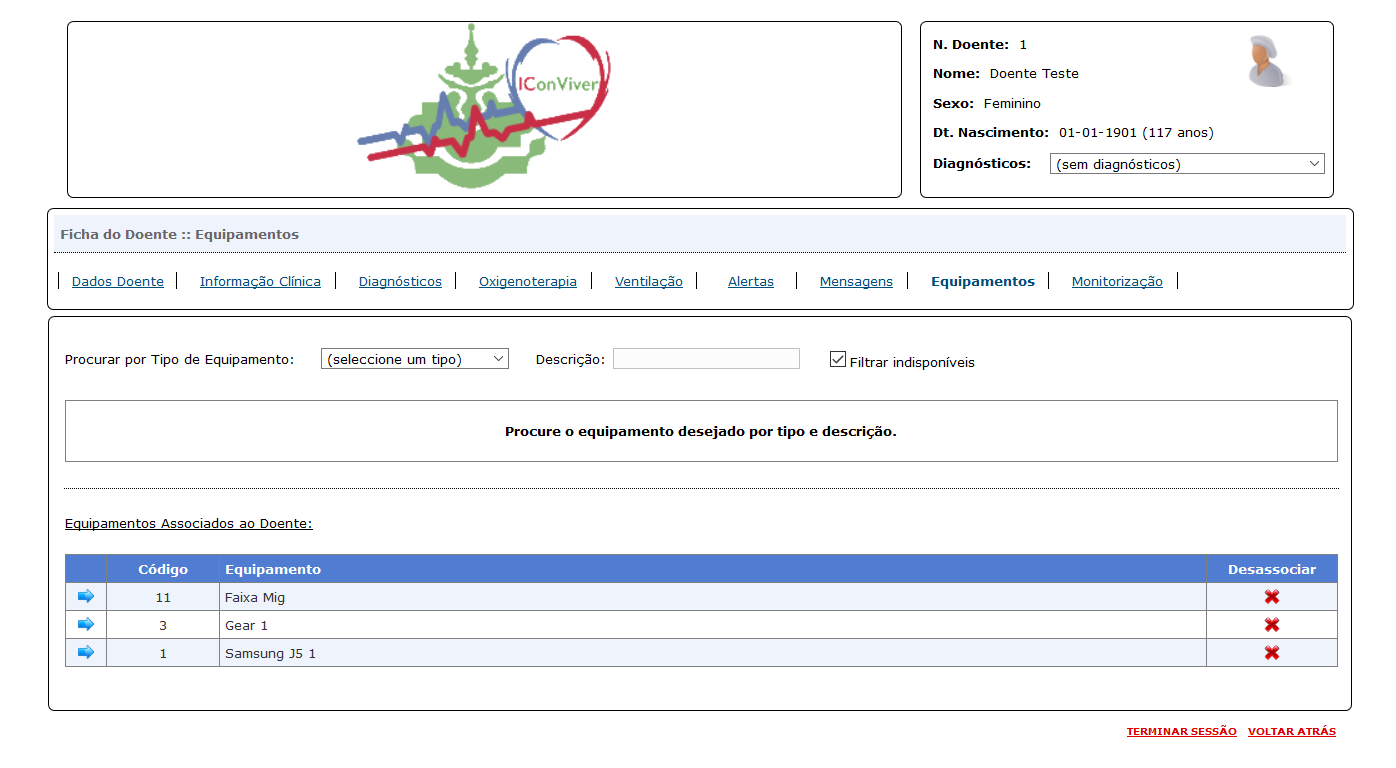
\includegraphics[width=0.85\textwidth]{dispositivos.png}
	\captionsetup{width=0.8\textwidth}
	\caption{Data visualization screen where one can choose the variables to see and their time frame.}
	\label{figure:UI5}
\end{figure}%

\begin{figure}[h!]
	\centering
	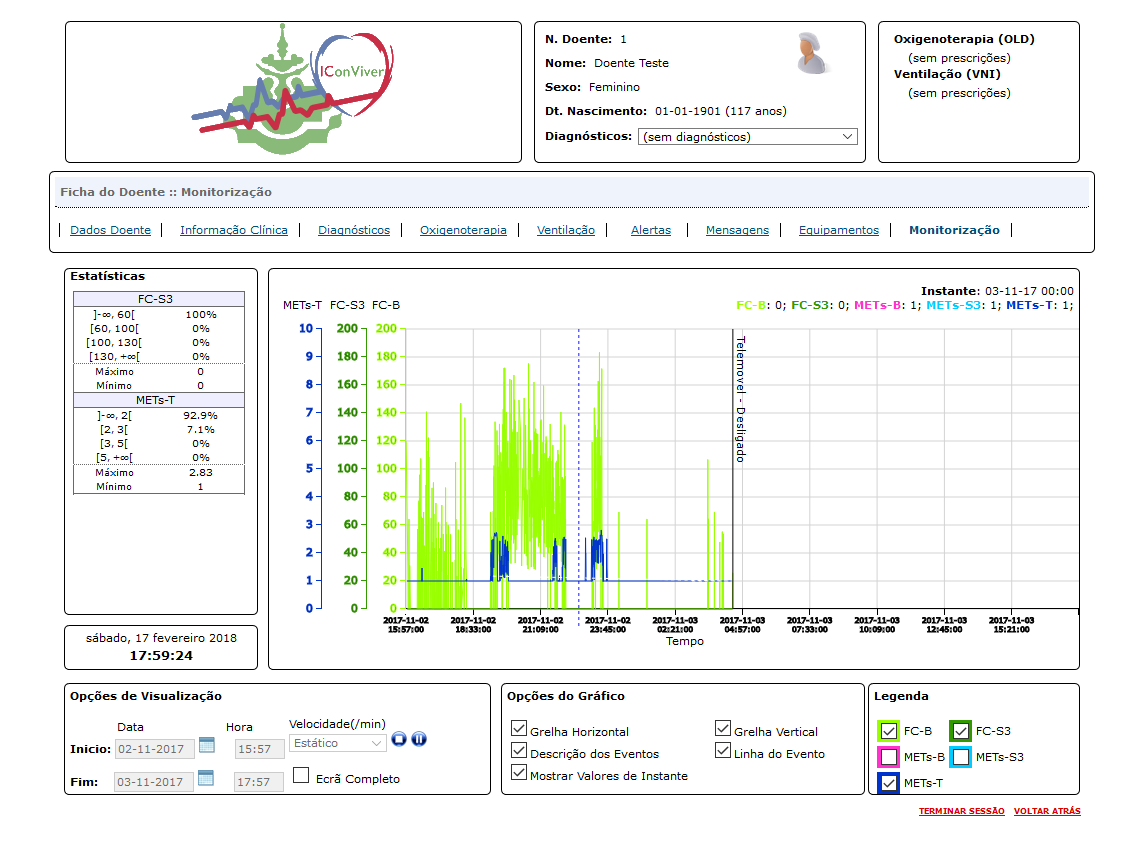
\includegraphics[width=0.75\textwidth]{data3.png}
	\caption{Data visualization screen where one can choose the variables to see and their time frame.}
	\label{figure:UI3}
\end{figure}%

Software for the server was adapted from software already implemented  for a different project \cite{telemold} by \ac{insticc}. All parameters and information to be passed to the remote device can be configured using the web interface and any numerical data coming from it can be shown in an interactive panel as well as warnings and events.

All aspects of the \ac{ui} were designed to provide a simple and versatile interface that can be used to interact with very different types of variables coming from a multitude of sensors. The main goal was to have a single interface that could be used in various contexts inside and out of hospital applications, and capable of being easily used with many variables and sensors.

The server itself is a computer with windows operative system and an internet connection that acts as a central control unit for the whole system. It is responsible for serving the user web interface, relaying information between the user and the devices and finally store all the information into a database. The interface is based in the .NET framewok with a Windows SQL Database.

System works with three major components:

\begin{itemize}
	\item \textbf{Web interface -} This is an ASP.NET website served using Windows Internet Information Services where user can configure all patient, device and acquisition parameters that are then stored into the database
	\item \textbf{Socket -} This component is in fact the two different subcomponents that ensure the communication between remote devices and the database.
	\begin{itemize}
		\item A .NET script is constantly waiting for socket connections and sends acquisition parameters to remote devices. It also receives and stores data sent from the devices containing patient processed data like \ac{hr} and \ac{mets} values.
		\item A Python script also constantly waiting for socket connections in a different port. This script is responsible for receiving and storing realtime raw data that may be sent by remote device (only active if raw data is requested).
	\end{itemize}
	\item \textbf{Database -} This component is responsible for receiving and storing all data that comes from all other components.
\end{itemize}

Two different socket processes were implemented to prevent clogging which could lead to data being lost. Also different languages were used for implementation convenience.

%\bigskip
%\textcolor{red}{\Large \textbf{Incompleto, imagens dos paineis e lista das costumizaçoes que podem ser feitas}}
%\bigskip

%\begin{figure}[h!]
%	\centering
%	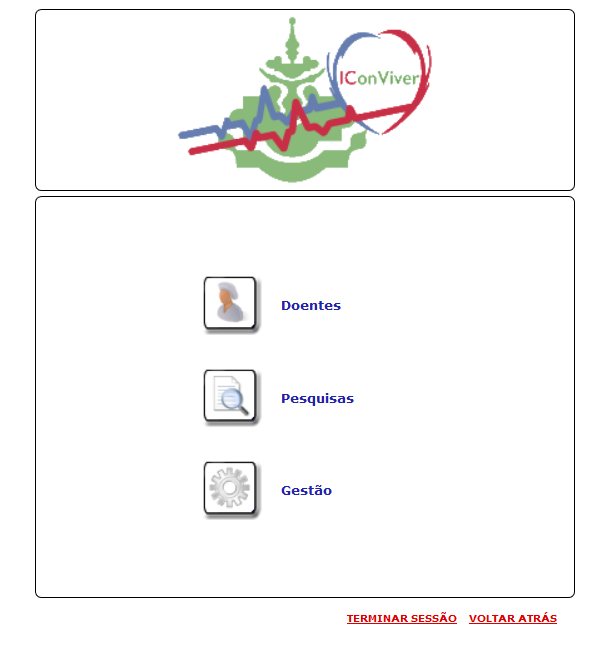
\includegraphics[width=0.45\textwidth]{login2.png}
%	\captionsetup{width=0.4\textwidth}
%	\caption{Initial panel after login into the system's web interface. Here one can see patient information; search for specific data of a particular patient; configure all device and acquisition parameters.}
%	\label{figure:UI1}
%	
%\end{figure}%
%
%\begin{figure}[h!]
%	\centering
%	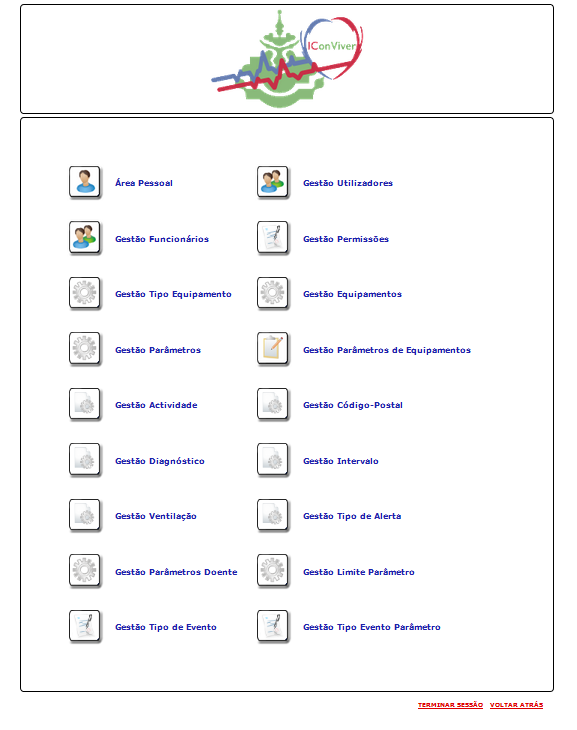
\includegraphics[width=0.85\textwidth]{gestao.png}
%	\captionsetup{width=0.8\textwidth}
%	\caption{Management screen, where all the systems and device's parameters can be defined.}
%	\label{figure:UI_gestao}
%	
%\end{figure}%
%
%\begin{figure}[h!]
%	\centering
%	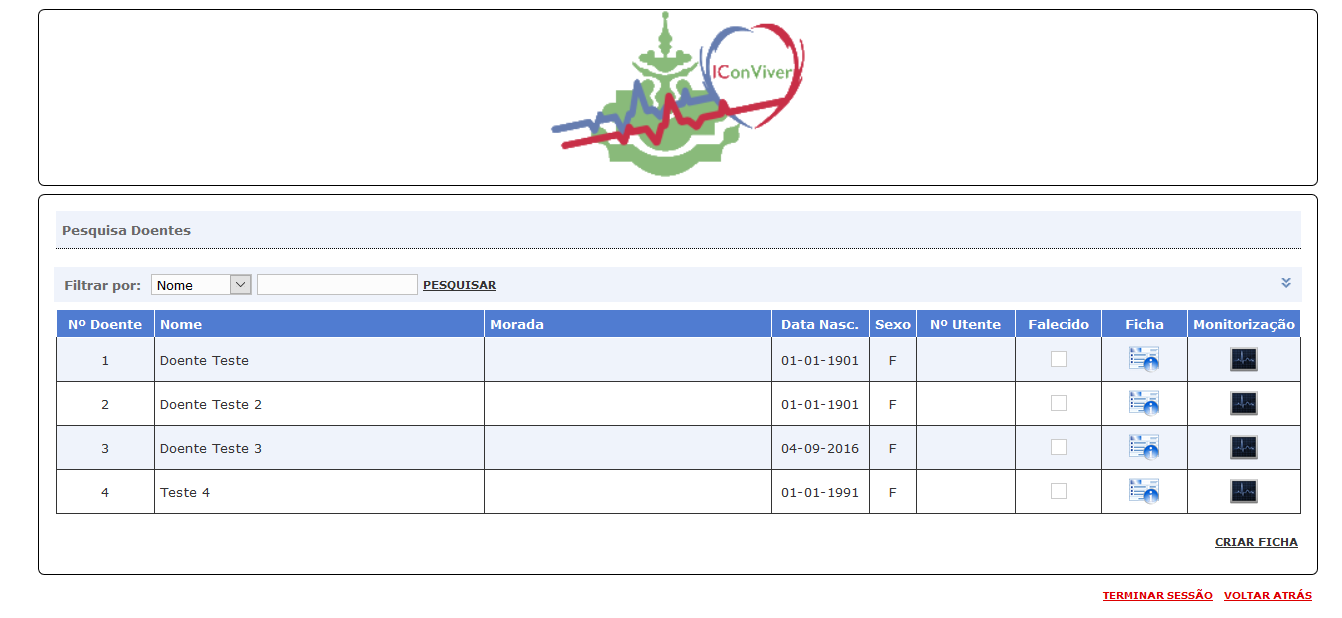
\includegraphics[width=0.85\textwidth]{doentes2.png}
%	\captionsetup{width=0.8\textwidth}
%	\caption{Screen showing the patients enrolled in the system. From here one can access all the information and collected data from each patient.}
%	\label{figure:UI2}
%\end{figure}%
%
%
%\begin{figure}[h!]
%	\centering
%	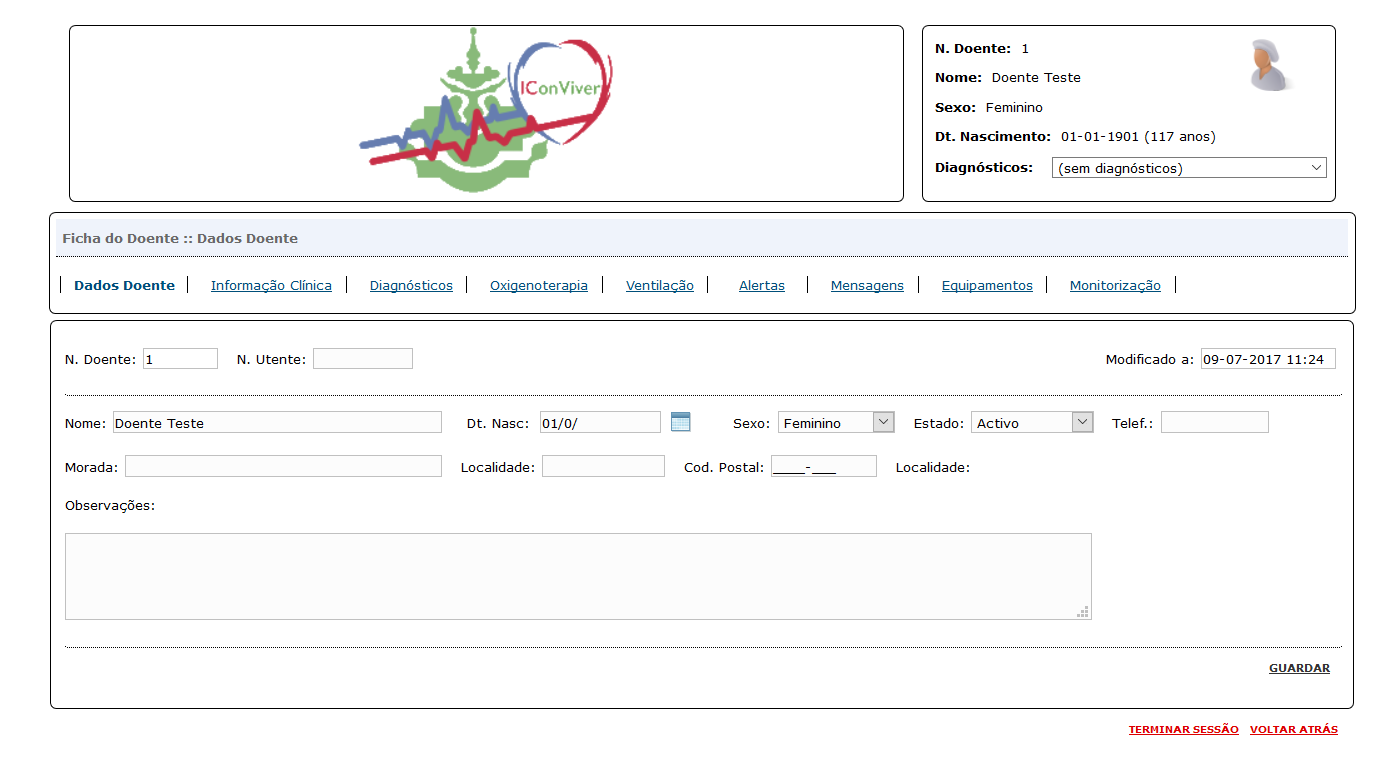
\includegraphics[width=0.85\textwidth]{paciente.png}
%	\captionsetup{width=0.8\textwidth}
%	\caption{Data visualization screen where one can choose the variables to see and their time frame.}
%	\label{figure:UI4}
%\end{figure}%
%
%\begin{figure}[h!]
%	\centering
%	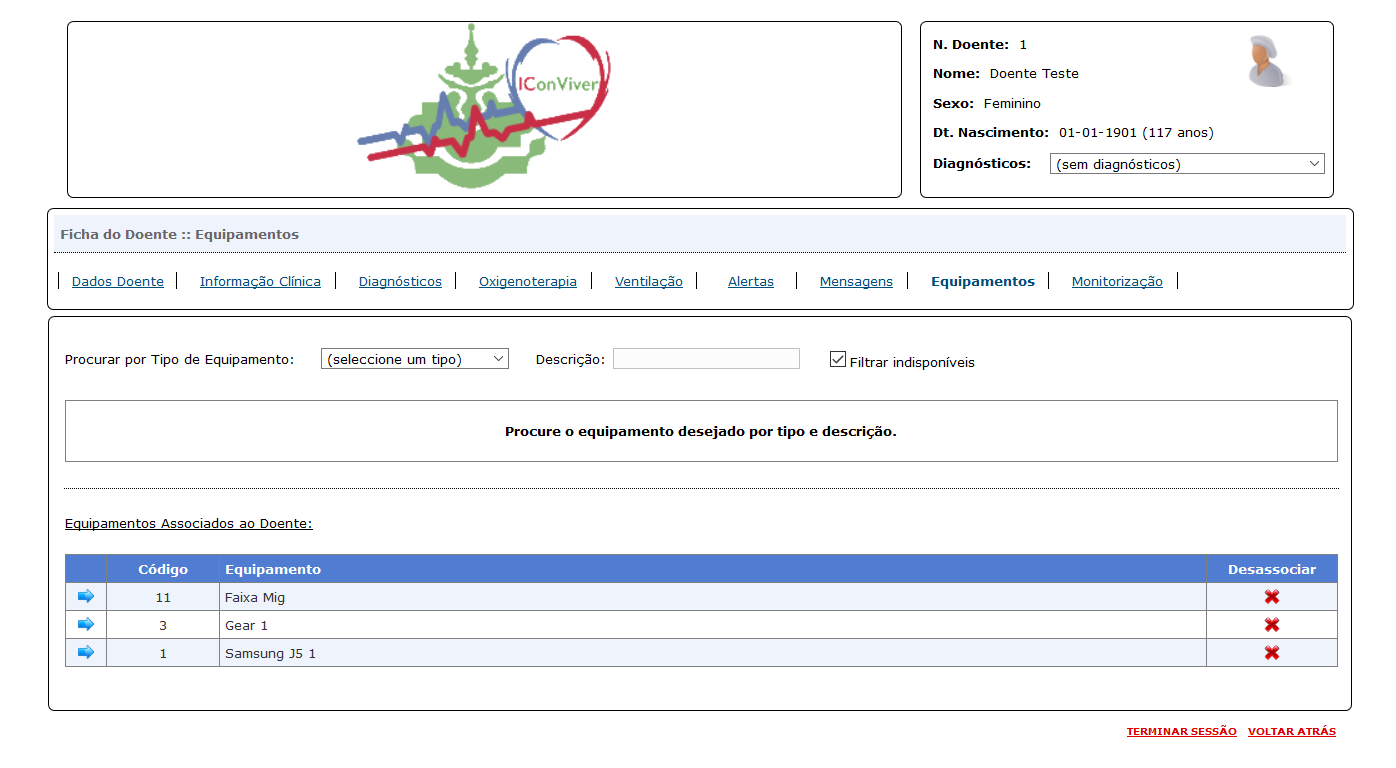
\includegraphics[width=0.85\textwidth]{dispositivos.png}
%	\captionsetup{width=0.8\textwidth}
%	\caption{Data visualization screen where one can choose the variables to see and their time frame.}
%	\label{figure:UI5}
%\end{figure}%
%\begin{figure}[h!]
%	\centering
%	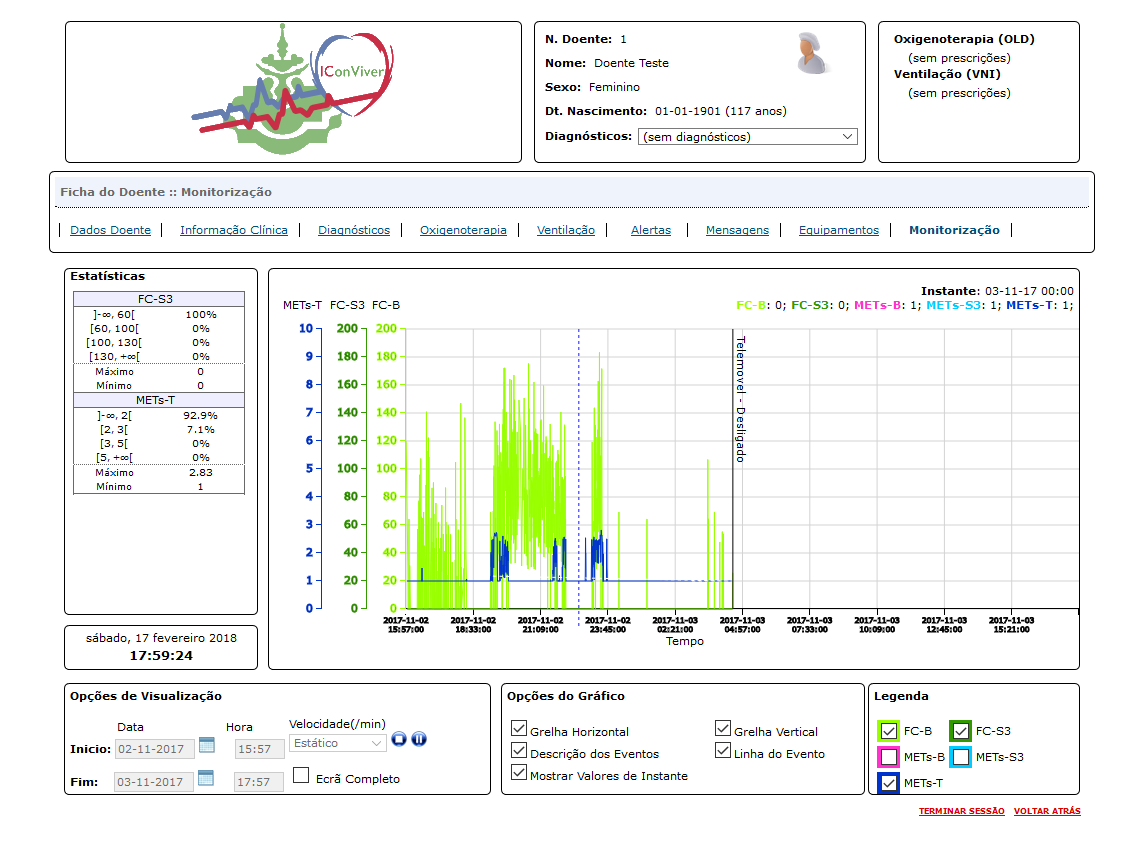
\includegraphics[width=0.75\textwidth]{data3.png}
%	\caption{Data visualization screen where one can choose the variables to see and their time frame.}
%	\label{figure:UI3}
%\end{figure}%

\Cref{figure:UI1,figure:UI_gestao, figure:UI2,figure:UI3,figure:UI4,figure:UI5} show some examples of the implemented web user interface, from where medical teams can control and configure all stages of the patient monitoring. From this interface medical teams can configure and access all information in the system ensuring the system is versatile to deal with many use cases.

\FloatBarrier
\subsubsection{Initial Server Configuration}



In order to setup the system to start acquisition, some parameters need to be configured in the management (Gestão) screen showed in \cref{figure:UI_gestao} that are accessed from screen in \cref{figure:UI1} after successful login.

Parameters to be configured on system setup:

\begin{enumerate}
	\item Devices connected to the system are categorized into types like smartphones or chest bands or others. The names of these types of devices are completely configurable, but to prevent mistakes only one device of each type can be assigned to a patient simultaneously. Each type of devices is identified by a name and single character code e.g. an S for smartphones.
	
	\item For each type of device it is required to define which parameters they need, these parameters must include a key parameter that includes the \ac{uuid} of the device labeled with the identifier "I". Other parameters can be configured but they vary based on the implemented features and support from the Android app, however they tend to be related with what sensors are active in each remote sensors and with what frequency they acquire and transmit data. These parameters are sent to the smartphone when it is turned on and are interpreted or relayed to the remote devices depending on the implemented interactions.
	
	\item It is also required to define what variables are to be displayed in the data visualization screen from \cref{figure:UI3}. To do this user must define the name of the variable, its range and the color of the corresponding line in the plot panel. Furthermore user can define intervals of values to see later the percentage of data that lies inside those intervals. This statistics can be seen in left panel of \cref{figure:UI3}.
	
	\item Optionally medical teams can configure rules that trigger an notification e.g \ac{hr} is below 50\ac{bpm} for more than 2minutes. To configure this rules, one should select a variable, a reference value, a relation between them (\textless, \textgreater or =) and a duration.
\end{enumerate}

\subsubsection{Acquisition Start}

In order to start data acquisition it is necessary to add patient information in screen showed in \cref{figure:UI4} and add the devices that should be active with that patient in screen of \cref{figure:UI5}. After this step, the smartphone and all other devices can be turned on and acquisition starts with data being displayed in panel of \cref{figure:UI3}. As data is received from the remote devices, it is displayed and user can chose to see data from a specific time-interval or to see data as it arrives in real time. From the web interface it is also possible to send text messages to the smartphone given to the patient.

All this configuration steps are necessary to ensure compatibility with any sensor medical teams consider adequate, making the system able to deal with any peculiarities each sensor may have.

Steps necessary for rotine aquisition start are presented in \cref{apendix:userguide}.

\section{Communication Protrocol}

\Cref{apendix:system} Details this topic.

When the smartphone is turned on, the application starts its execution and sends an initial message to the server containing a timestamp and its own \ac{uuid}. The server then responds with n identic messages, where n is the number of remote/wearable sensors. These messages contain the code number of the patient, a timestamp, the UUID of the remote sensor, the type of the remote sensor (smartwatch, smartphone, etc...) and pairs of (name, value) for all the custom parameters that user defined in the configuration.
The first and last character of these handshake messages is the special mark "\textbackslash".

After this initial handshake, the smartphone periodically sends data to the server in a similar fashion, the message is composed of a timestamp, the patient code number and pairs of (name, value) for each of the variables that are being sent. For this messages, the first and last character is \#.

Other messages are exchanged including alerts and events, each type having a similar structure, timestamp, patient code, and pairs of values and identifications containing the UUID of the relevant device and the respective error or event code. Each type of message has a special character that is repeated in the begining and end of the message.

Regarding the communication between the remote sensors and the smartphone, this is a very variable protocol as it depends on the peculiarities of each sensor utilized, and for this reason no standard protocol is defined.

%The first message sent by the smartphone:
%
%%\begin{verbatim}
%%  \ 1417162942424 0019B9FBE258 \
%%  1      2             3       4
%%\end{verbatim}
%
%\begin{table}[h!]
%%	\small
%	\begin{tabular}{>{\color{pgrey}}c >{\color{pgrey}}c >{\color{pgrey}}c >{\color{pgrey}}c}
%		\textit{\textbackslash}  & \textit{1417162942424}  & \textit{0019B9FBE258} & \textit{\textbackslash} \\
%		 & \textit{timestamp} & \textit{UUID}  &   \\ 
%	\end{tabular}
%\end{table}
%
%
%%\begin{enumerate}
%%	\item char \
%%	\item long - timestamp
%%	\item 6 hex - UUID
%%	\item char \
%%\end{enumerate}
%
%The server response for each remote device:
%
%
%1.	/ (char) - inicio da mensagem
%2.	(long) – hora da comunicação
%3.	(int) – código do doente que se está a ligar
%4.	(int) – período de comunicação entre cliente e servidor (em segundos)
%5.	(char) – equipamento
%6.	(6 hex) – mac address do equipamento
%7.	(char float)[] – pares de parâmetro  e valor referentes à configuração do equipamento
%8.	/ (char) – fim da mensagem
%
%
%\begin{table}[h!]
%	%	\small
%	\begin{tabular}{>{\color{pgrey}}c >{\color{pgrey}}c >{\color{pgrey}}c >{\color{pgrey}}c}
%		\textit{\textbackslash}  & \textit{1417162942424}  & \textit{0019B9FBE258} & \textit{\textbackslash} \\
%		& \textit{timestamp} & \textit{UUID}  &   \\ 
%	\end{tabular}
%\end{table}



\section{Privacy}
\label{chapter:privacy}

Regarding data transmissions between devices, privacy was also a concern. Having smartphnes connected through mobile data connectivity the chances of intercepting data are smaller when comparing with the hypothesis of having devices connected through wifi. Also Bluetooth connectivity is encrypted, so data coming from the wearable sensors is also secured.

Data is stored in the database in a completely anonymous form i.e. the patient information is stored separately, each patient is assigned a number, and is identified by that number in all other processes. Furthermore, when the smartphone connects to the server and sends data, it is always sent being labeled by only the patient's number.

Using a login system, it is possible to define for every user of the system, if the patient's informations are visible or not, further increasing security, not allowing everyone to access the user interface. % file "Thesis_Implementation.tex"
\cleardoublepage

\input{DataProcessing} % file "Thesis_Implementation.tex"
\cleardoublepage


\chapter{System Evaluation}
\label{chapter:evaluation}

The system was used and tested on patients with cardiac diseases from Hospital de Santa Marta - CHLC (Lisbon) and the main variables collected were heart rate (HR) and Metabolic Equivalent of Tasks (METs) \cite{crouter_METS}. These variables were indicated by the hospital's cardiology team as being common variables used in their practice to diagnose and track patients \cite{importancia_HR_METS, importancia_HR_METS_2}. Variables to be collected determined the type of sensors needed.

Devices utilized to test this system were chosen as they provide cost effective platforms to support the desired functions. Cost and quality were taken into account and established market products were preferred as they offer greater consistency in quality over time and over numbers i.e. it is easy to ensure the good working of the system even if more devices are added after some time and they can be added in larger numbers to use with more patients.

\begin{figure}[!h]
	\centering
	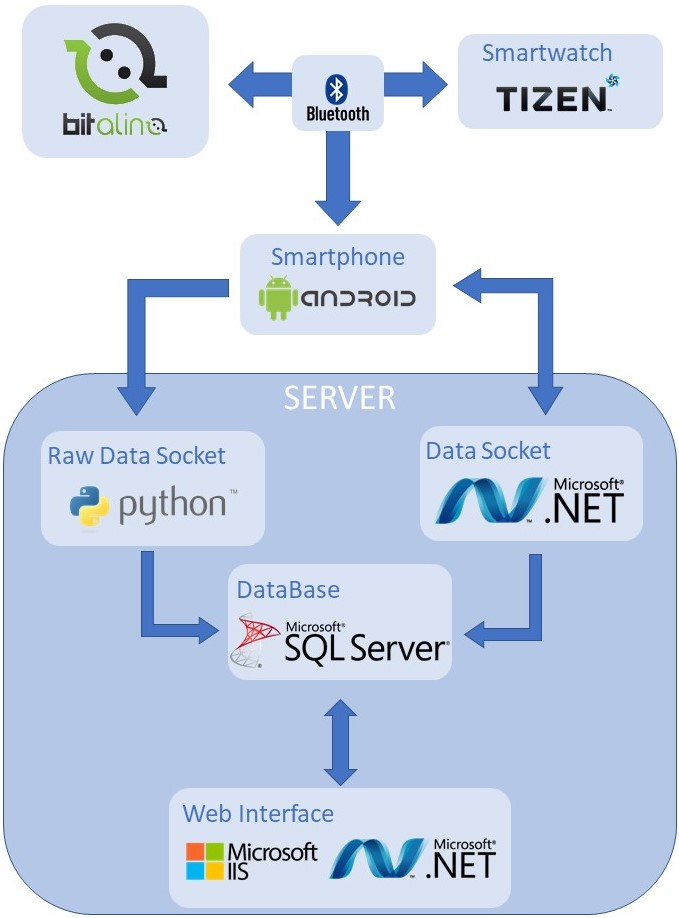
\includegraphics[width=0.75\textwidth]{platforms.jpg}
	\caption{Platforms and programing languages used to build and run the system. Choice of platforms were based on device}
	\label{fig:platforms}
\end{figure}

After all hardware and software was finished the system was tested in lab and hospital conditions. The main objectives of the tests were to assess system's usability, concerning comfort and ease of use by patient and doctor. Another major objective of testing the system was to verify the accuracy and reliability of the sensors utilized and the robustness of all the software, data transmissions and storage. All the software components were tested individually but still real life situations brought to light some minor bugs that were corrected once detected. Another major concern to be tested was loss of data during transmissions.

The devices used in the present work are directed to patients diagnosed or with suspects of cardiac insufficiency, hence the most relevant variables to collect are related with heart rate (HR) and accelerometry as a way of estimating the level of physical activity during the patients' daily life. To collect this data 3 devices were used, each with different sensors as detailed in \cref{table:vars}. Complete system architecture for the testing phase is depicted in \cref{fig:platforms}.

\begin{table}[!h]
	\centering
	\caption{Variables acquired by each device and the corresponding information extracted. 
		CD - Chest Deflection (respiratory frequency); PA - Physical Activity (measured in METs); ACC - Accelerometry}
	\label{table:vars}
	\begin{tabular}{|c|c|c|c|}
		\hline
		\textbf{Device } & \textbf{Variables} & \textbf{Sampling Rate (Hz)} & \textbf{Extracted information} \\ \hline
		\multirow{3}{*}{Smartwatch} & PPG       & 25                 & HR                    \\ \cline{2-4} 
		& HR        & 25                 & HR                    \\ \cline{2-4} 
		& ACC       & 100                & PA                    \\ \hline
		\multirow{3}{*}{BITalino}   & ECG       & 1000               & HR                    \\ \cline{2-4} 
		& ACC       & 1000               & PA                    \\ \cline{2-4} 
		& CD        & 1000               & RR                    \\ \hline
		Smartphone                  & ACC       & 100                & PA                    \\ \hline
	\end{tabular}
\end{table}

\FloatBarrier

\section{Wearable Sensors}

\subsection{Smartwatch}

The smartwatch used was the Samsung Gear S3 and it's function is to collect data and send it to the smartphone, acting like a sensor. This device was chosen as a way to reduce the patient's discomfort, as it can be a less invasive sensor, replacing the watch  many use daily. Another reason for the choice of this device was its novelty, as it was a new model at the time devices were chosen for this work, and it was expected to perform better than every previous smartwatch. Finally, the choice of this highly capable and versatile smart device was made with future developments in mind as it allowed for more functionalities to be implemented, like its use as a data hub (replacing the smartphone) and even allowing for an interface so the patient could interact with the system using only the smartwatch.
It has several sensors, including luminosity, atmospheric pressure, PPG, ACC and others decribed in \cite{Tizen_sensor}. %https://developer.tizen.org/development/api-references/native-application?redirect=/dev-guide/2.3.1/org.tizen.native.mobile.apireference/group__CAPI__SYSTEM__SENSOR__MODULE.html#ga41397923efb60755882608685edf1ecb
This device also has another "sensor" that produces values of instantaneous HR calculated from PPG data.

\subsubsection{Tizen App}

A native application software was developed to collect data from the desired sensors and send it, through BT, to the smartphone.
This smartwach's operative system (OS), Tizen, supports applications written in C language using many functions provided specifically for this OS.

When app is first initialized, a Bluetooth server is mounted awaiting for incoming connection from the smartphone. To prevent app being interrupted when screen is off, it is needed to lock CPU in on state and also, initialize sensors API with the appropriate option.

Code responsible for initializing the app Bluetooth server and sensors with the correct formulaion to prevent unintentional deactivation:

\bigskip
\begin{lstlisting}[language=C++]
#include <bluetooth.h>
#include <app_control.h>
#include <glib.h>
#include <stdlib.h>

static bool app_create(void *data){
	int server_socket_fd = -1;
	bt_adapter_state_e bt_ad_state = BT_ADAPTER_DISABLED;
	
	device_power_request_lock( POWER_LOCK_CPU, 0);
	
	bt_initialize();
	bt_adapter_get_state(&bt_ad_state);
	
	if (bt_ad_state != BT_ADAPTER_DISABLED) {
	} else {			
		bt_socket_create_rfcomm(BT_MGR_UUID, &server_socket_fd);
		bt_socket_set_connection_state_changed_cb(_socket_conn_state_changed_cb);
		bt_socket_listen_and_accept_rfcomm(server_socket_fd, MAX_NUM_PENDING);
	}
	
	data_initialize(data, update_sensor_values);

	if(feedback_initialize() == FEEDBACK_ERROR_NONE){
		feedback_play_type(FEEDBACK_TYPE_VIBRATION ,FEEDBACK_PATTERN_LOWBATT);
		feedback_play_type(FEEDBACK_TYPE_VIBRATION ,FEEDBACK_PATTERN_BT_CONNECTED);
		feedback_play_type(FEEDBACK_TYPE_VIBRATION ,FEEDBACK_PATTERN_BT_DISCONNECTED);
		feedback_play(FEEDBACK_PATTERN_LOWBATT);
		feedback_play(FEEDBACK_PATTERN_BT_CONNECTED);
		feedback_play(FEEDBACK_PATTERN_BT_DISCONNECTED);
	}

	return true;

}

bool data_initialize(void *data, Update_Sensor_Values_Cb sensor_update_cb)
{
	int i=0;
	
	//sensor_type_e sensors_list[] = {SENSOR_ACCELEROMETER, SENSOR_LIGHT, SENSOR_PRESSURE, SENSOR_HRM, SENSOR_HRM_LED_GREEN};

	sensor_type_e sensors_list[] = {SENSOR_ACCELEROMETER, SENSOR_HRM, SENSOR_HRM_LED_GREEN};

	for (i = 0; i < SENSOR_COUNT; ++i) {
		sensor_get_default_sensor(sensors_list[i], &sensors[i].handle);
		sensor_create_listener(sensors[i].handle, &sensors[i].listener);
		sensor_listener_set_option(sensors[i].listener, SENSOR_OPTION_ALWAYS_ON);
		sensor_listener_set_event_cb(sensors[i].listener, LISTENER_TIMEOUT, sensor_update_cb, i);
		sensor_listener_start(sensors[i].listener);
	}
	return true;
}

void update_sensor_values(int count, float *values, sensor_type_e type, appdata_s *ad)
{

// Manipulate sensor's values

}
\end{lstlisting}
\bigskip

When a Bluetoth connection is established, a particular message 'go' must be sent to initialize data collection. Other messages are available to stop the acquisition 'quit' or to request battery information 'batt'.

Code used to get battery status and percentage:

\bigskip
\begin{lstlisting}[language=C++]

device_battery_level_e battery_status = DEVICE_BATTERY_LEVEL_EMPTY;

int battery_percent = 0;

device_battery_get_percent(&battery_percent)

device_battery_get_level_status (&battery_status)

\end{lstlisting}
\bigskip

To interact with the sensors, a manufacturer provided API was used. It is built in a logic of callbacks, i.e. an event is generated when the sensor value changes.
Sampling rate is defined to be the default for each sensor that, according with the manufacturer guide, can range between 100Hz and 1 HZ \cite{Tizen_sensor} meaning that events occur at different rates for different sensors. 

To have a uniform sampling protocol, a buffer is kept containing the current value of each sensor and whenever a sensor event occurs, the corresponding values in this buffer are updated. In parallel, in another thread, there is a timer running at 100Hz that takes a snapshot of values in the buffer and writes them into a different array accompanied by a timestamp of the moment the snapshot was taken. Data from all sensors is held and when the array has 10 seconds of data, it is sent to the smartphone. This transmission strategy was implemented as a way of reducing the overhead of sending samples in real time, at 100Hz, which had a larger battery consumption and also induced the loss of samples, reported by the BT API provided by the manufacturer, returning an error for every message lost. The buffer technique was used as a very easy and simple way of upsampling data from sensors with a sampling frequency lower than 100Hz using a sample and hold method.

\begin{figure}[!h]
	\centering
	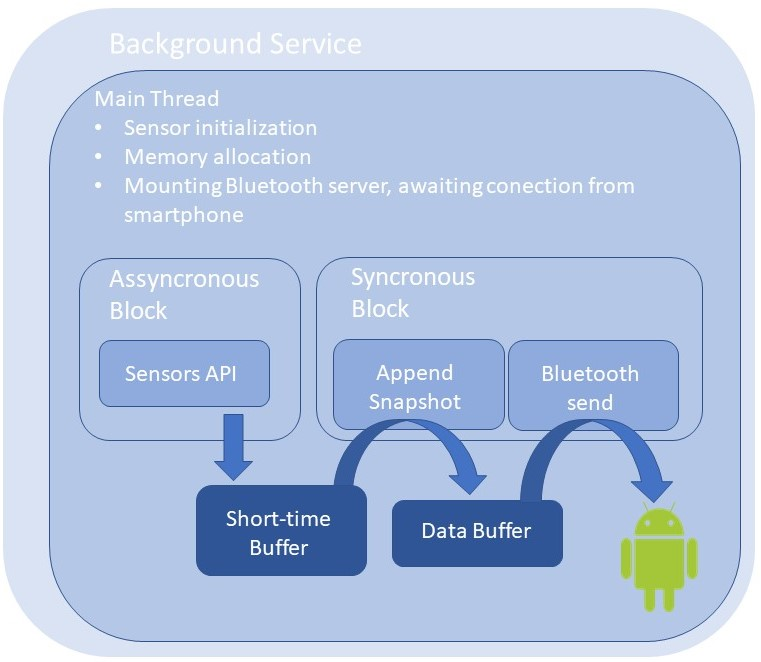
\includegraphics[width=0.75\textwidth]{app_tizen.jpg}
	\caption{Smartwatch App threads call-stack}
	\label{fig:app_tizen}
\end{figure}

\Cref{fig:app_tizen} shows the implemented app architecture having two main components, an asynchronous and synchronous block. The first runs when a sensor reports a new sample and its callback ir triggered. This function updates the buffer value that corresponds to the sensrs that triggered its callback. The other block that runs periodically and appends the current buffer values to another, larger, array, that stores 10s of data. This block is also responsible for sending the data when the 10s of data is collected, clearing the storage array.

%https://developer.tizen.org/development/api-references/native-application?redirect=/dev-guide/2.3.1/org.tizen.native.mobile.apireference/group__CAPI__SYSTEM__SENSOR__MODULE.html

%https://developer.tizen.org/development/api-references/native-application?redirect=https://developer.tizen.org/dev-guide/2.3.1/org.tizen.native.mobile.apireference/group__CAPI__SYSTEM__SENSOR__INFORMATION__MODULE.html

%http://www.mdpi.com/2075-4426/7/2/3/html

%https://news.samsung.com/global/in-depth-look-the-parts-and-pieces-that-make-the-gear-s3-tick

\begin{figure}[!h]
	\centering
	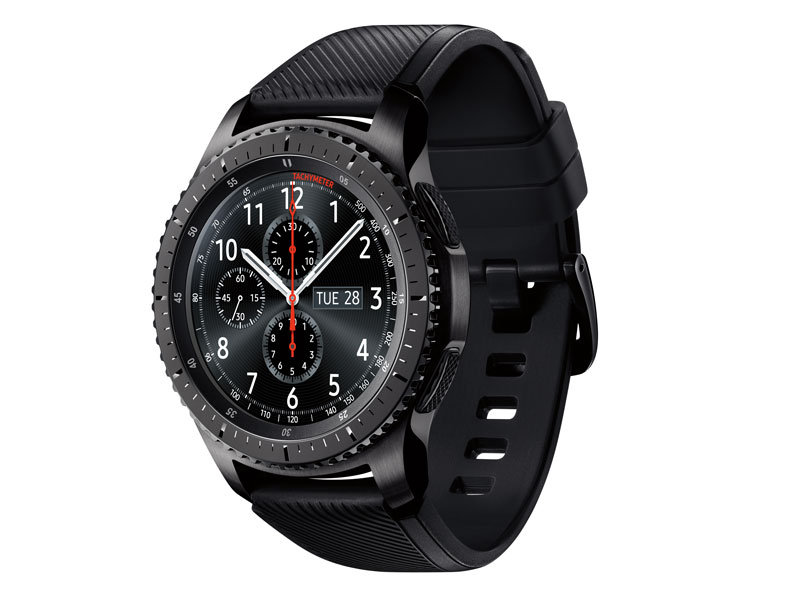
\includegraphics[width=0.5\textwidth]{samsung-gear.jpg}
	\caption{Smartwtch Samsung Gear S3 Frontier}
	\label{fig:watch}
\end{figure}

\FloatBarrier

\subsection{BITalino}

%This device was used as a mean of validating the measurements of other sensors, more specifically to provide a reference to compare with the HR estimation made by the smartwatch.

BITalino\cite{bitalinoguerreiro2013bitalino}  was used in the form of a chest band that collects various signals and sends them to the smartphone via BT. In particular it was chosen because it provides a high quality ECG signal \cite{bitalinobatista2017experimental,bitalinoguerreiro2013bitalino} that complemets the information collected by the smartwatch. BITalino was used, also, because it was a familiar tool that fitted the requirements to provide a ground truth to the other sensors used in the system. Initially the use of this device was meant to be as a validation tool and would not be used once the system was fully operational and the number of monitored patients increased. But the relevance of the information provided by the ECG signal it collected justified its presence in the context of cardiac patients monitoring.

A chest band was built in order to accommodate the sensors enumerated in \cref{table:vars} with a comfortable and practical form-factor. This was a major concern as patients comfort was very important to ensure success of the system, once it was intended to be used for long periods of time. Because of this, also battery size was an issue. Stock BITalino battery has 700mAh of capacity, but to eliminate any chance of this not being enough, a 1300mAh was used (\cref{table:battery}).

Apart from the electronic components, the chest band was built using a standard commercial chest band from Polar\textregistered  used for sports tracker devices. This was a very good base as this band had several positive aspects:

\begin{itemize}
	\item It had sown into the fabric two conductive rubber pads from which ECG could very easily be collected.
	\item Elastic and adjustable bands with easy to use locks, meaning it was very easy to put on and take off while ensuring a good fit to most patients.
\end{itemize}

To ensure protection of the electronics components, a tough fabric cover was sewn into the elastic band with holes for the on/off switch and charging port.

\begin{figure}[!h]
	\label{fig:faixa}
	\makebox[\linewidth][c]{%
		\begin{subfigure}[t]{0.5\textwidth}
			\centering
			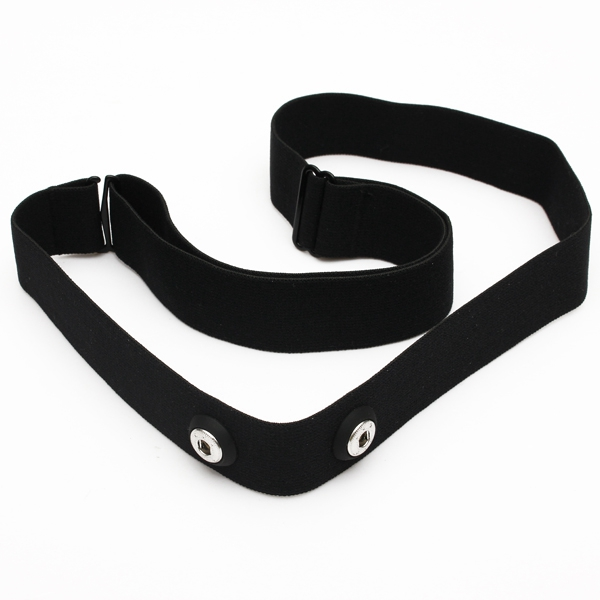
\includegraphics[width=0.8\textwidth]{faixa.jpg}
			\caption{Polar\textregistered  band that served as base for the BITalino components.}
		\end{subfigure}%
		\begin{subfigure}[t]{0.5\textwidth}
			\centering
			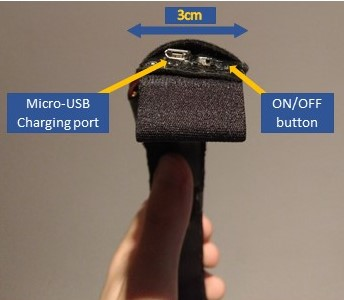
\includegraphics[width=0.8\textwidth]{faixa_botao.jpg}
			\caption{Charging port and on/off switch.}
		\end{subfigure}%
	}\\
	\caption{Chest band.}
\end{figure}

%\textcolor{red}{\Large \textbf{escala da figura esta estranha}}

\begin{figure}
	\centering
	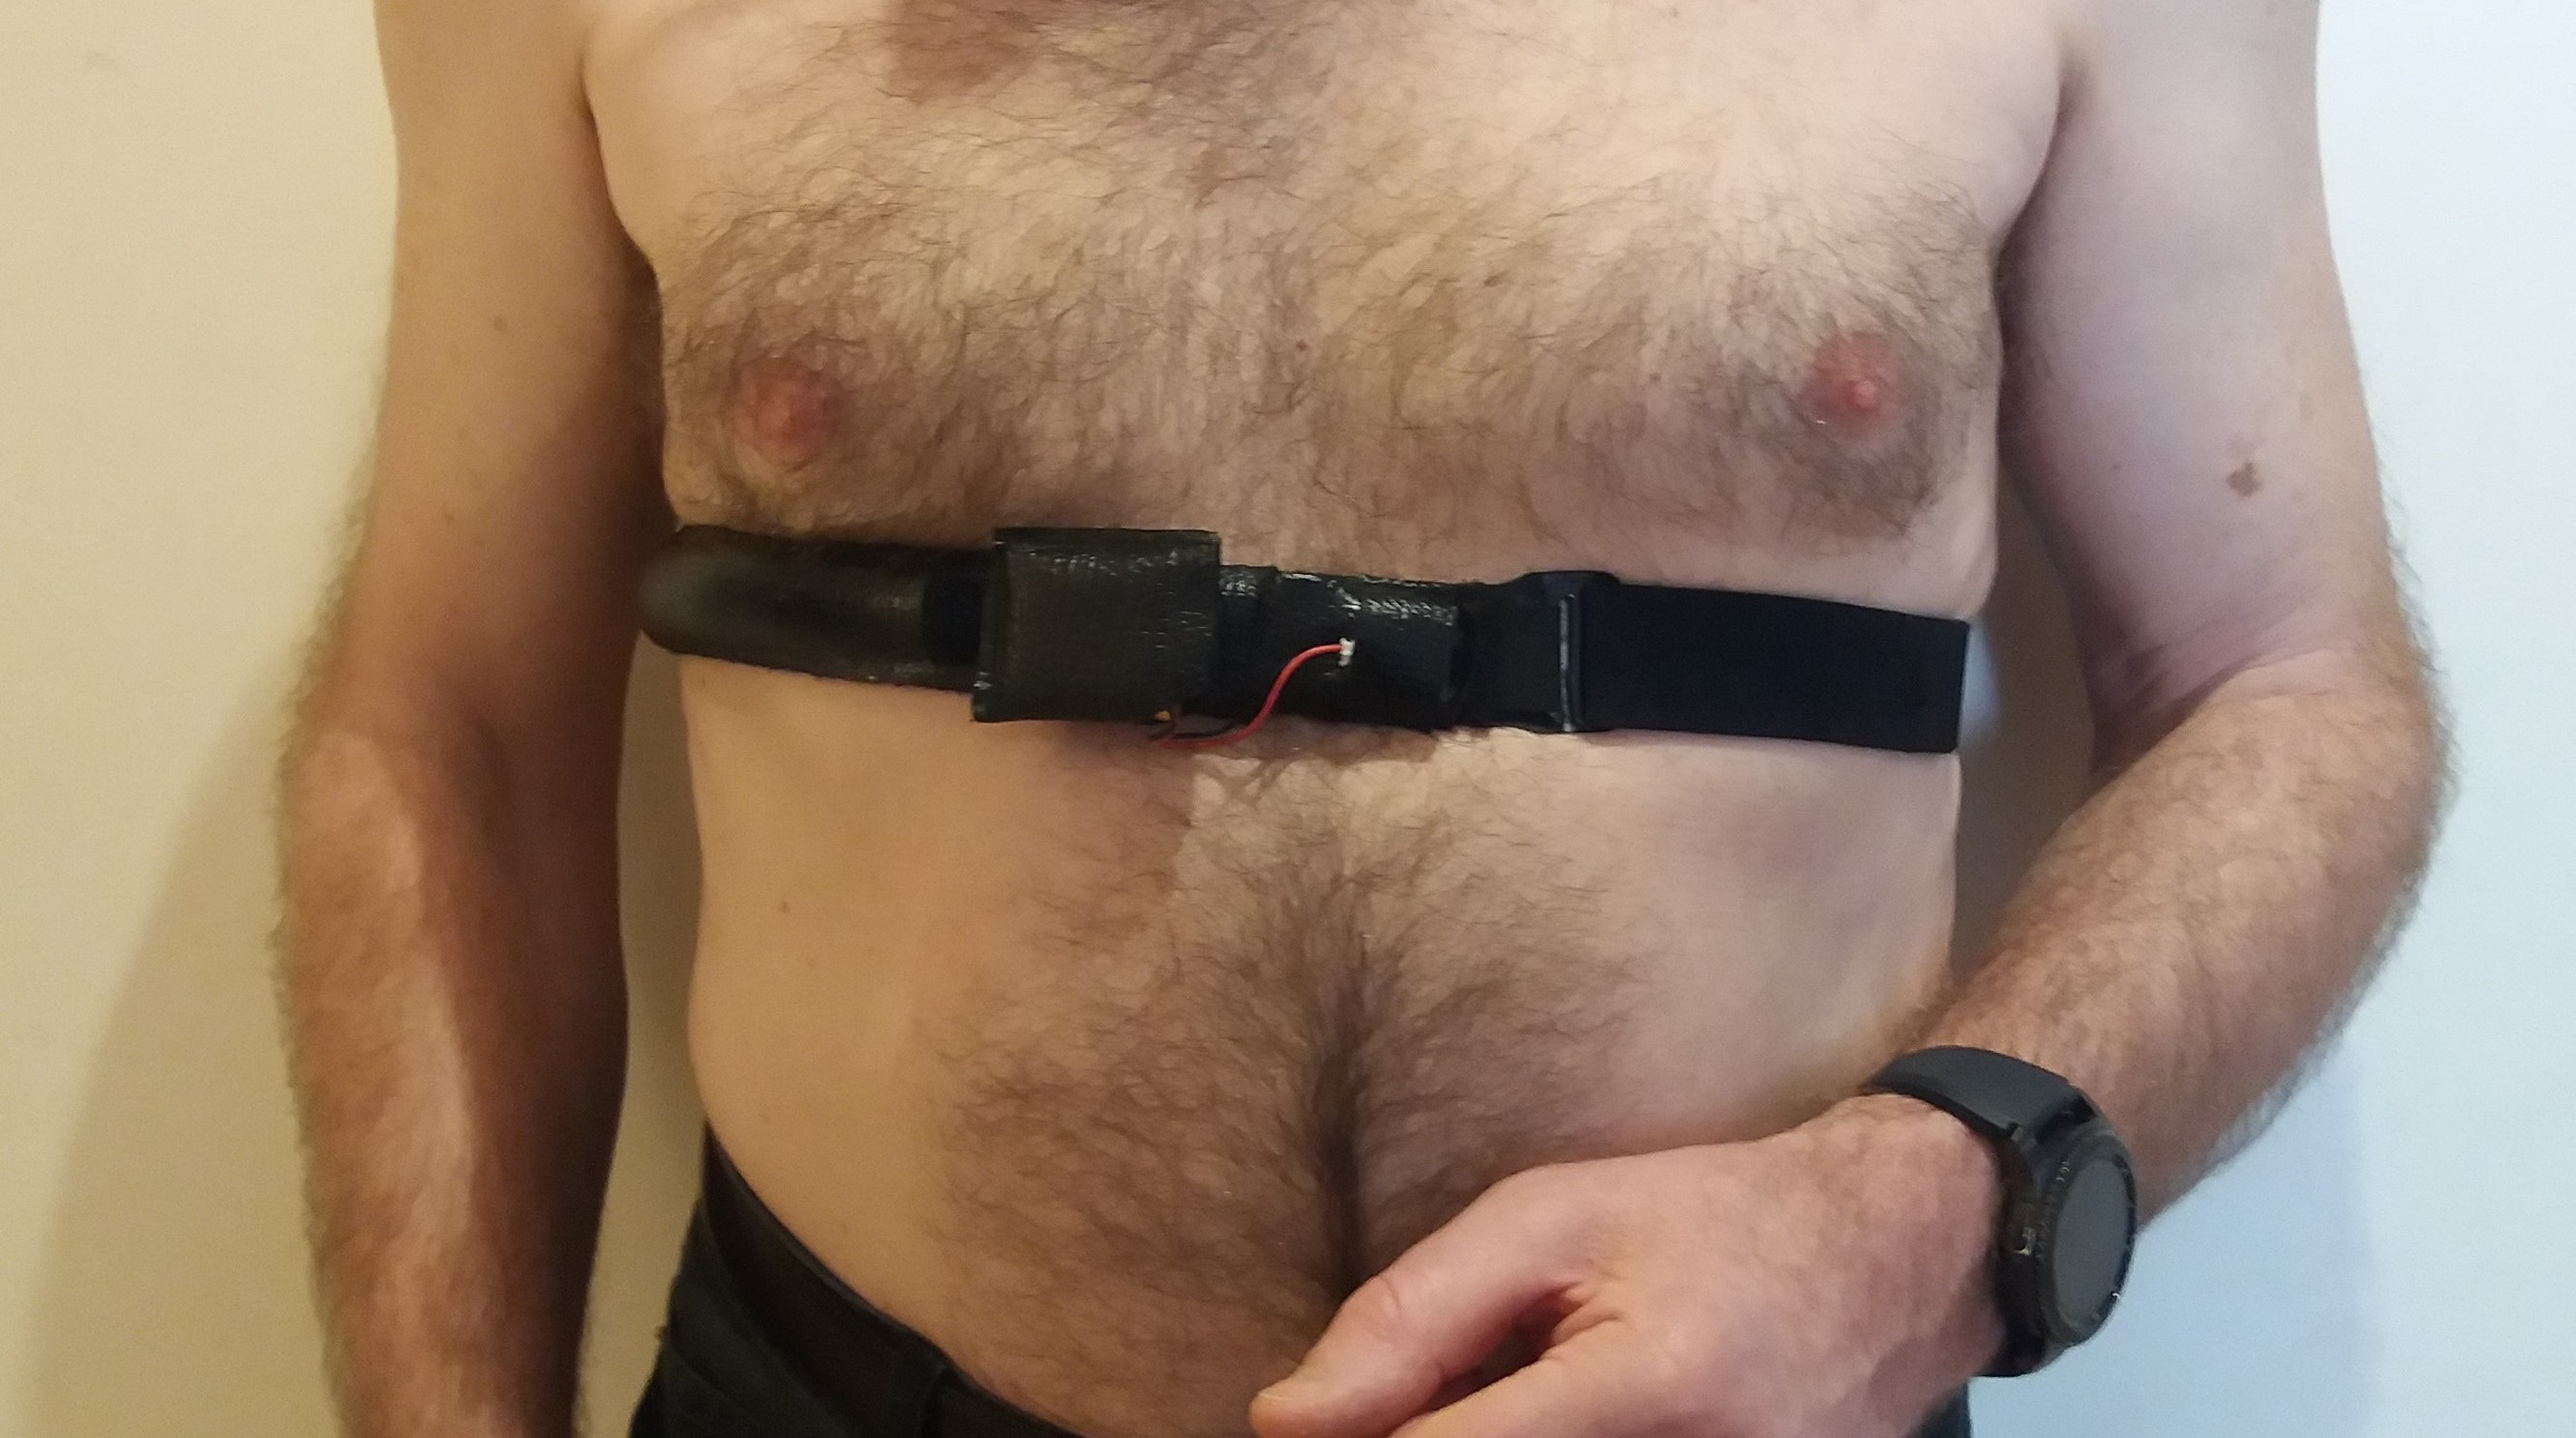
\includegraphics[width=0.6\linewidth]{setup}
	\caption{Patient wearing the selected sensors.}
	\label{fig:setup}
\end{figure}


\FloatBarrier

\section{Comfort and Usability}

As mentioned before, comfort and ease of use for patient and physician were two major concerns when designing and choosing all hardware and software features.

For the patient the importance of these aspects comes from the fact that system is meant to be used continuously for long periods of time and if the system becomes a hassle it is harder to get patient's compliance and get useful data. It was also very important that all interfaces and charging procedures were as simple as possible. This was important because great part of the patients to be monitored are elderly and in some cases even illiterate so simplicity was a major concern. For this, on screen battery information and sound notifications were utilized to notify the patient to charge the devices when needed (\cref{fig:app}).

To ensure practicality and ease of use for physicians and medical staff, requisites were to have a simple web interface (\cref{apendix:userguide}) in what concerns patient enrollment into the platform, and data visualization.

All of these aspects were assessed along the design process and were put to test in hospital context. 

During the design process students were asked to wear the system and report on aspect to be improved relating with comfort and ease of use.

As an initial hospital test, a medical team from cardiology service was given all the equipment and, using the guides provided in \cref{apendix:userguide}, fitted the system into a 72 year old male patient. Following this the patient wore the system for 24 hours and reported the experience.

From this experience the comments that emerged were mostly related with charging procedures. Web, Android and Tizen interfaces were considered very convenient and simple to use. Battery life was one of the main aspects referred as to be improved by the medical professionals. This led to the introduction of a power bank for the smartphone and a bigger battery for the chest band to ensure battery life expectations were met. Despite efforts, concerning software optimization and increased battery sizes, \cref{table:battery} still depicts slightly shorter-than-optimal battery life-times.

Another negative aspect reported was the difficulty with charging the chest band. As a safety measure, BITalino does not charge the battery while acquiring data, this was designed to guarantee isolation of the patient from the electricity mains. Although this feature creates an additional step of turning the chest band on and off when charging, the main problem reported by medical teams had to do with the toggle button. This is a very small component, as shown in \cref{fig:faixa}, which was considered difficult to use due to its size. Although it was a very valid comment, to change it, a major redesign of the chest band was required since all alternative buttons had a significantly larger size and for this reason, this aspect was left unchanged for the course of this work.

Overall the system had very positive feedback by all participants, patients and medical teams. On the medical personnel side, the system worked well as a data acquisition platform with minimum configuration required, and interfaces were considered very convenient, presenting very useful information. On the patients side there was an unexpected effect, besides considering the system comfortable to wear with minimum disturbance of their daily-life, patients reported to feel more accompanied and better taken care knowing that they are being monitored 24hr a day. This was not expected initially and may contribute to even better outcomes, as feeling more taken care of may improve patients' health status acting similarly to the placebo effect.

\begin{table}[!h]
	
	\centering
	\caption{Battery lifetime of acquisition devices}
	\label{table:battery}
	\begin{tabular}{|c|c|c|}
		\hline
		\textbf{Device}		 		&
		\textbf{Conditions}		&
		\textbf{Duration} \\ \hline
		\multirow{3}{*}{Smartphone}      &  Connected only to Smartwatch & 13h 30min  \\ \cline{2-3} 
		& Connected to BITalino and Smartwatch                                 &    11h 30min      \\ \cline{2-3} 
		& Connected to BITalino, Smartwatch and power bank                                                              &  \textbf{16h 30min}        \\ \hline
		BITalino
		& With 1300mAh battery                                                                              & 48h     \\ \hline
		Smartwatch                        & -----                                                                                             &  12h 30min        \\ \hline
	\end{tabular}
\end{table}

\section{Communications}

In order to determine if data transmission was occurring without losses nor delays, each message had a mark to allow its localization in time. For communications between the smartphone and BITalino, a sequence number is included and allows to determine if there are missing messages by checking the increment of this number. For messages between  the smartphone and Gear S3 a timestamp was sent with each message and data loses can be detected by checking the time delay between consecutive messages.

To assess the situations that led to data loss, this sequence numbers and timestamps were checked while the system was acquiring data. Distance is one of the factors that may contribute for packets being lost in transmission, although, during the normal use of the system, distances are rather short so it is not expected that this interferes with message transmission. In fact the only situation where data loss systematically occurred was when the smartphone was requesting a Bluetooth connection i.e. if the smartphone is already receiving data from device A and is trying to connect with device B, some packets coming from A are lost. Otherwise the system performed in a very robust way concerning data transmissions.

\section{Heart Rate Estimation from PPG data}

In order to evaluate the accuracy of HR estimates given by Samsung Gear S3, the later was used to record HR in different situations with several subjects with and without cardiac pathologies. Simultaneously a BITalino  \cite{bitalinoguerreiro2013bitalino} and a medical-grade certified device were used to determine the HR from ECG data and provide a ground truth reference for Gear's values.

\subsection{Methodology}

\subsubsection{Experimental Protocol}
\label{chapter:experiments}

To validate heart rate values calculated by Gear S3 three experiments were conducted:
\begin{itemize}
	\item E1 - Consisted on acquiring data for short periods of time with subjects performing a specific activity:
	\begin{itemize}
		\item Resting state, moving as least as possible (2min)
		\item Walking at a regular pace (5min)
		\item One subject was asked to pedal on a  stationary bike  at moderate pace (5min)
		\item One subject was asked to run at moderate pace (2min)
	\end{itemize}
	Some of these acquisitions were repeated to verify reproducibility and infer on system robustness.
	\item E2 - On this experiment, data was recorded for periods between 1 and 2 hours while subjects performed their usual activities during their daily lifes.
	%with 3 young healthy subjects (all 23 years old)
	\item E3 - The experiment consisted on collecting data from 3 hospitalized patients with various cardiac diseases during a stress test, taking place at hospital.
	These tests consisted of patients walking on a treadmill, increasingly fast until they are not able to continue, followed by a rest period. Patients ECG and energy consumption are monitored while executing the task. The procedure was performed according to Bruce protocol \cite{bruce}.
	%with ages (47, 42,\textcolor{red}{\Large \textbf{Idades}})
\end{itemize}


\subsubsection{Test Equipment}

Multiple devices were used to evaluate subjects' HR:

\begin{itemize}
	
	\item Samsung Gear S3 Frontier - HR is calculated by the smartwatch from PPG data using manufacturer's algorithm, as detailed in \cref{chapter:hr_bvp}.
	\item A BITalino based chest band, collecting one derivation ECG at 1000Hz, with HR estimation being made according with \cref{chapter:hr_ecg}
	\item For stress tests HR information is also collected by a Mortara XScribe 3.10.10 by Mortara Instrument \cite{mortara} that collects 12 lead ECG, producing a very reliable HR estimate as it is a certified medical device.	
	
\end{itemize}

\subsubsection{Accuracy Measurement}

The accuracy of the HR values produced by the smartwatch, and also  the ones estimated from the ECG signal, was summarized as statistics of the absolute error (AE) e.g. mean absolute error (MAE) as defined in \cref{eq:mae}.

\begin{equation}
AE_i = \left|{HR}_i^{true} - {HR}_i^{est}\right|
\label{eq:ae}
\end{equation}

\begin{equation}
MAE = \frac{1}{N}\sum_{i=0}^{N}\left|{HR}_i^{true} - {HR}_i^{est}\right|
\label{eq:mae}
\end{equation}

\begin{conditions}
	N     & nr. of HR values estimated for a subject \\
	{HR}_i^{true} 	& Ground-truth value of HR for ith 10s signal window \\
	{HR}_i^{est}    & Estimated value of HR for ith 10s signal window \\   
\end{conditions}

This measurement was chosen as it provides an easy and fast interpreting quantity to be known and used by physicians when analyzing patient data. Furthermore, unlike usual metrics like percent error, absolute error is completely independent from HR range which is a desirable feature as, ideally, the precision should be high for all HR ranges, and there is no reason for errors at higher HR values being less important.

\FloatBarrier
\subsection{Experimental Setup and Results}

Data was collected from two separate groups performing different activities. Stress tests were undertaken by 3 patients with various cardiac conditions and ages 42, 47 and 50 years old. The other experiments enumerated in \cref{chapter:experiments} were performed by 3 healthy volunteers all 23 year olds. In following figures and tables Si denotes subject i and Tj denotes jth trial.

After data collection from subjects, the first observation of the PPG signal revealed the vast influence of motion artifacts (MA). This is depicted in \cref{figure:raw}. When the subject is completely immobile it is easy to find, even by inspection, a correlation between ECG and PPG signal peaks (\cref{figure:raw_repouso}) corresponding to systolic peaks. The same is not true when the subject is moving, as signal corruption greatly affects PPG signal and correlation is no longer obvious and maybe not present at all (\cref{figure:raw_movimento}).


\begin{figure}[!h]
	\centering
	%	\makebox[\linewidth][c]{%
	\begin{subfigure}{0.5\textwidth}
		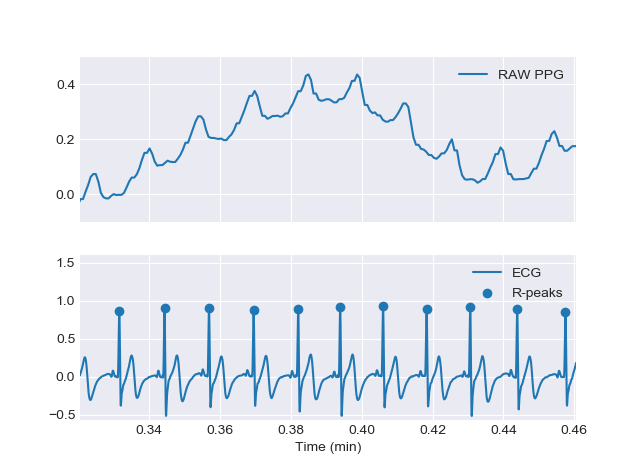
\includegraphics[width=\textwidth]{raw_repouso1.png}
		\caption{Raw signal while completely immobile. HR calculated from PPG (first curve): 75bpm; HR calculated from ECG (second curve): 79bpm.}
		\label{figure:raw_repouso}
	\end{subfigure}
	\begin{subfigure}{0.5\textwidth}
		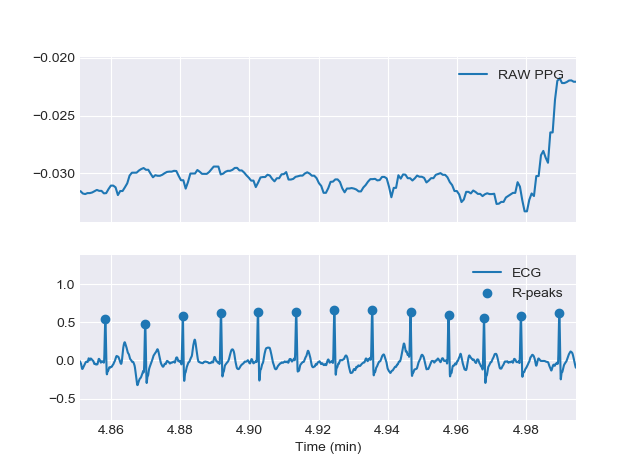
\includegraphics[width=\textwidth]{raw_movimento1.png}
		\caption{Raw signal while walking. HR calculated from PPG (first curve): 52bpm; HR calculated from ECG (second curve): 81bpm}
		\label{figure:raw_movimento}
	\end{subfigure}
	%	}\\
	\caption{Segments of raw signal captured by the sensors in different conditions with the synchronous identified R-peaks.}
	\label{figure:raw}
\end{figure}

Observing \cref{figure:hr_}, it is visible that Gear S3 is not capable of keeping up with fast variations in HR and \cref{figure:hr_hosp} clearly illustrates the difficulty in determining HR accurately during movement, with a very large estimation error being present, until subject enters the resting phase of the stress test.

%\begin{figure}[!h]
%	\centering
%%	\makebox[\linewidth][c]{%
%		\begin{subfigure}{0.45\textwidth}
%			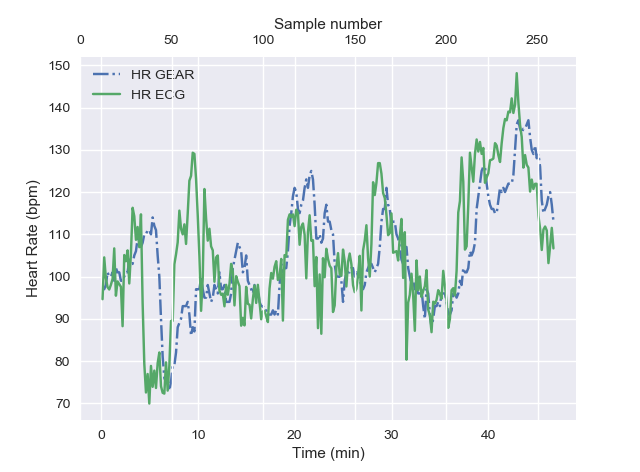
\includegraphics[width=\textwidth]{HR.png}
%			\caption{Heart Rate of subject during daily life activities.}
%			\label{figure:hr_}
%		\end{subfigure}
%		\begin{subfigure}{0.45\textwidth}
%			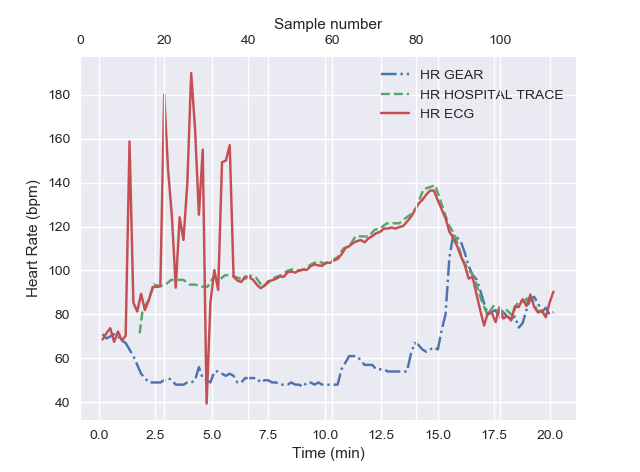
\includegraphics[width=\textwidth]{HR_hospital.png}
%			\caption{Heart Rate of subject during stress test.}
%			\label{figure:hr_hosp}
%		\end{subfigure}
%%	}\\
%	\caption{Example of HR curves obtained from  the various systems over two experiments, E1 (a) and E3 (b)}
%	\label{figure:hr}
%\end{figure}

%From the several algorithms used to process PPG data in an attempt to improve HR accuracy, none of them proved to behave better than the manufacturer's algorithm. This indicates a tailor made algorithm for this sensor in particular that is not easily replicated, even using very recently proposed state-of-the-art algorithms, as well as established methods. Having this into account, only Samsung's algorithm estimations will be considered henceforth.

%\FloatBarrier
\subsubsection{Short Acquisitions (E1)}


\begin{figure}[!h]
	\centering
	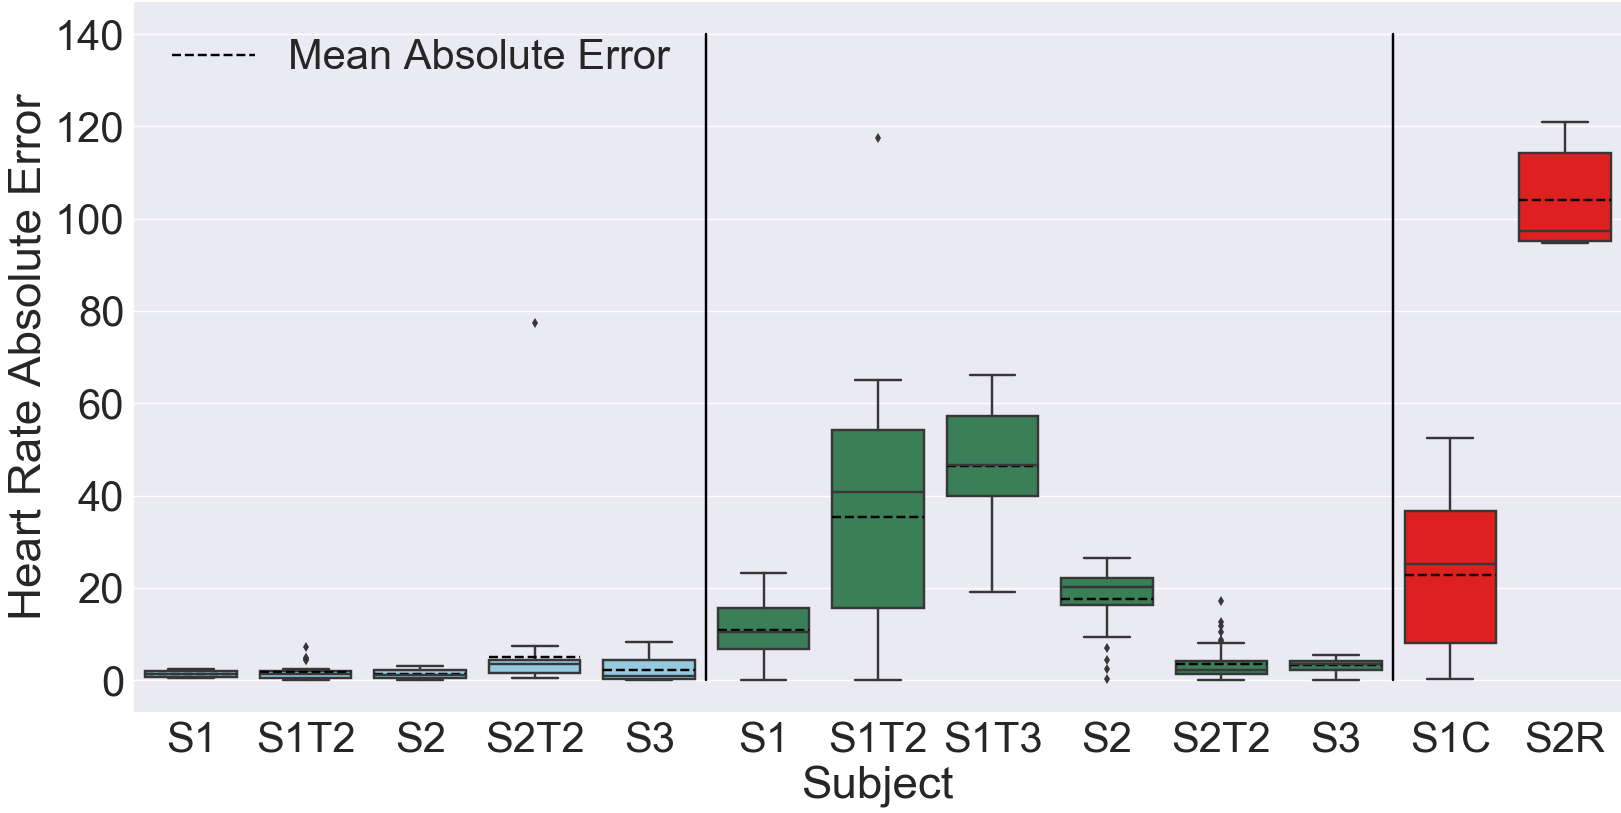
\includegraphics[width=0.85\textwidth]{box.png}
	\caption{Absolute Error of HR while performing different activities: (left) resting; (middle) walking; right cycling and running.}
	\label{figure:box}
\end{figure}

%This experiment's main activity was to determine the accuracy of the HR estimate made by the smartwatch based on the PPG data it collects, using ECG signal to provide a ground-truth.

When analyzing the absolute error of HR determined from the smartwatch's PPG data collected while subjects were performing specific activities, it is very obvious that motion highly corrupts sensor data and thus, greatly damages accuracy. In \cref{figure:box} is very clear a tendency to error increase as subjects go from resting to walking, cycling or running.
Another thing that can be noted in \cref{figure:box} and \cref{table:MAE} is the relatively large difference in the error values between subjects and trials. This may indicate low robustness of the device's measurements, as they are affected by sensor positioning, tightness and also by how the subjects move, as some individuals present accentuated arm movement which can further disrupt accuracy.

\begin{table}[!h]
	\centering
	\caption{Mean Absolute Error (MAE) of each experiment and activity averages.}
	\label{table:MAE}
	\begin{tabular}{|c|c|c|c|}
		\hline
		\textbf{Activity}                 & \textbf{Subject} & \textbf{MAE} & \textbf{Average}      \\ \hline
		\multirow{5}{*}{\textbf{Resting}} & S1               & 1.4          & \multirow{5}{*}{2.4}  \\ \cline{2-3}
		& S1T2             & 1.8          &                       \\ \cline{2-3}
		& S2               & 1.3          &                       \\ \cline{2-3}
		& S2T2             & 5.1          &                       \\ \cline{2-3}
		& S3               & 2.2          &                       \\ \hline
		\multirow{6}{*}{\textbf{Walking}} & S1               & 10.8         & \multirow{6}{*}{21.2} \\ \cline{2-3}
		& S1T2             & 35.3         &                       \\ \cline{2-3}
		& S1T3             & 46.4         &                       \\ \cline{2-3}
		& S2               & 17.7         &                       \\ \cline{2-3}
		& S2T2             & 3.4          &                       \\ \cline{2-3}
		& S3               & 3.3          &                       \\ \hline
		\textbf{Cycling}                  & S1               & 22.8         & \multirow{2}{*}{63.4} \\ \cline{1-3}
		\textbf{Running}                  & S2               & 104.1        &                       \\ \hline
	\end{tabular}
\end{table}

\FloatBarrier
\subsubsection{Daily life (E2)}
\FloatBarrier

\Cref{table:MAE_daily} and \cref{figure:box_daily} demonstrate clearly that during daily-life activities like walking or any activity that implies arm movement, Gear S3 has a poor performance as a sensor platform and, in certain occasions, it is not even possible to detect any type of signal trends. In a medical context, this could lead to gross errors when trying to diagnose or follow a patient, or it would require further tests which renders the pervasive monitoring less efficient or even counterproductive.

\begin{figure}[!h]
	\centering
	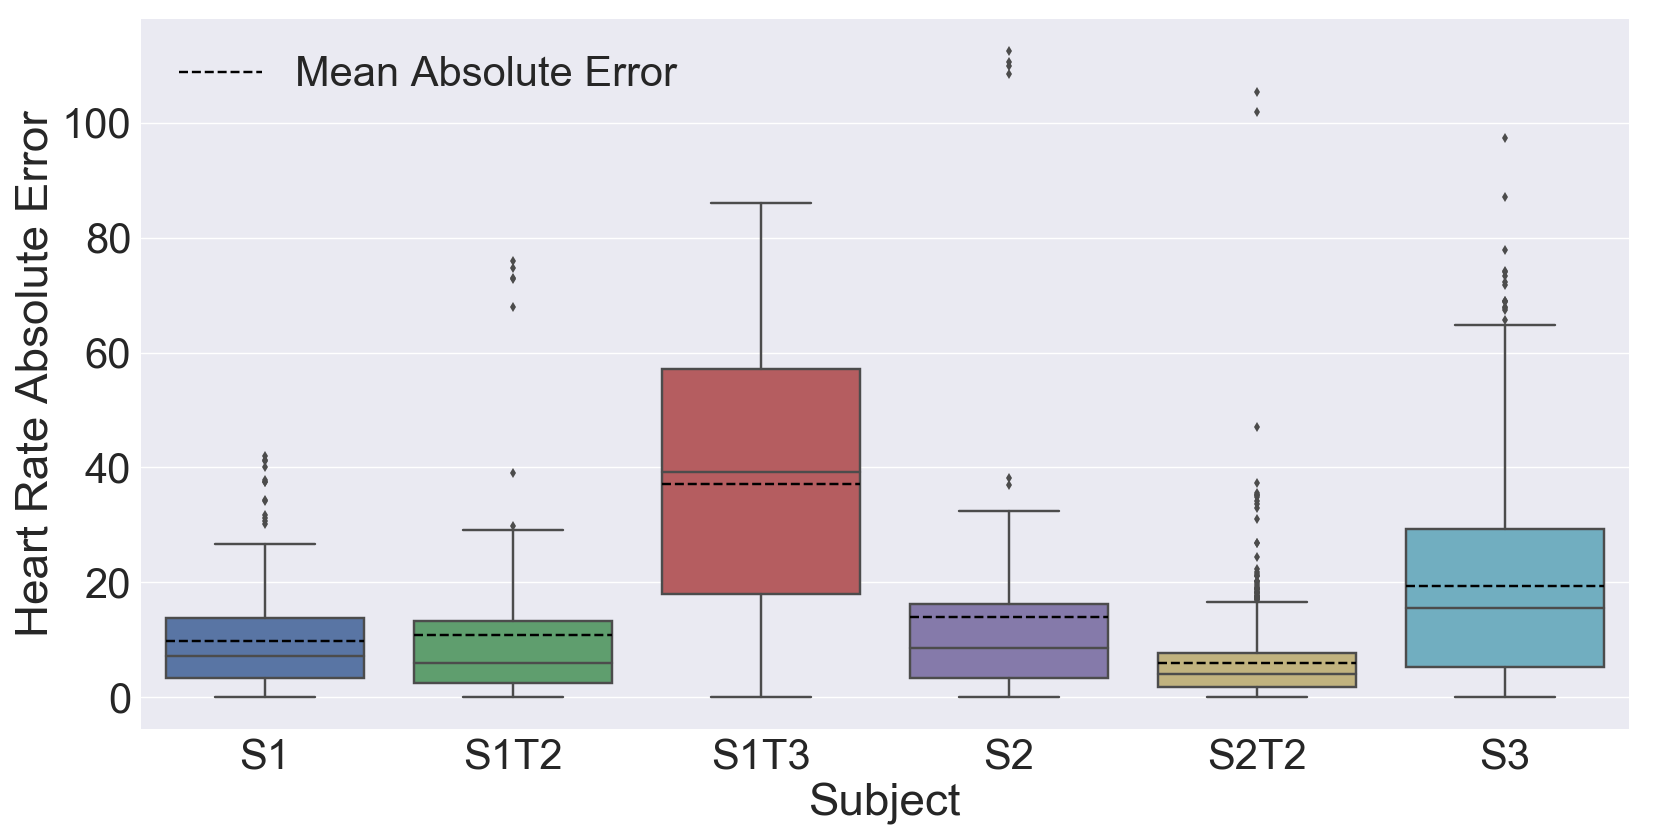
\includegraphics[width=0.85\textwidth]{box_daily.png}
	\caption{Absolute Error of HR while subjects perform their usual life activities (office working, walking, eating, etc...).}
	\label{figure:box_daily}
\end{figure}

\begin{table}[!h]
	\centering
	\caption{Mean Absolute Error (MAE) of each subject during daily life activities.}
	\label{table:MAE_daily}
	\begin{tabular}{|c|c|c|c|}
		\hline
		\textbf{Activity}                                                                         & \textbf{Subject} & \textbf{MAE} & \textbf{Average}      \\ \hline
		\multirow{6}{*}{\textbf{\begin{tabular}[c]{@{}c@{}}Daily-life\\ activities\end{tabular}}} 
		& S1               & 9.7          &\multirow{6}{*}{16.2} \\ \cline{2-3}
		& S1T2             & 10.8         &                       \\ \cline{2-3}
		& S1T3             & 37.1         &                       \\ \cline{2-3}
		& S2               & 13.9         &                       \\ \cline{2-3}
		& S2T2             & 6            &                       \\ \cline{2-3}
		& S3               & 19.3         &                       \\ \hline
	\end{tabular}
\end{table}

\begin{figure}[!h]
	\centering
	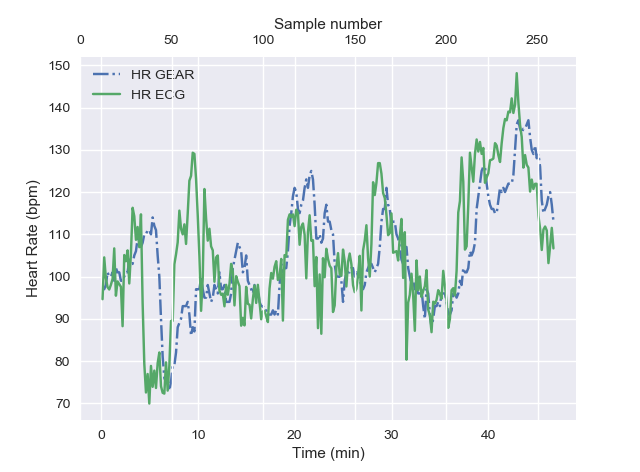
\includegraphics[width=0.85\textwidth]{HR.png}
	\caption{Example of HR curves obtained during daily life activities.}
	\label{figure:hr_}
\end{figure}


\subsubsection{Stress Test (E3)}

As expected, during a stress test, where the subject is moving with some intensity, HR determination error is very large and as can be seen in \cref{figure:hr_hosp}, error is specially large during the exercise phase of the stress test, supporting hypothesis of motion artifacts corrupting the signal.
Error during these tests reached \textgreater100bpm wich renders this sensor platform completely unfit for this kind of contextwhere precision is of utmost importance to avoid wrong diagnostics and treatments.

\begin{figure}[!h]
	\centering
	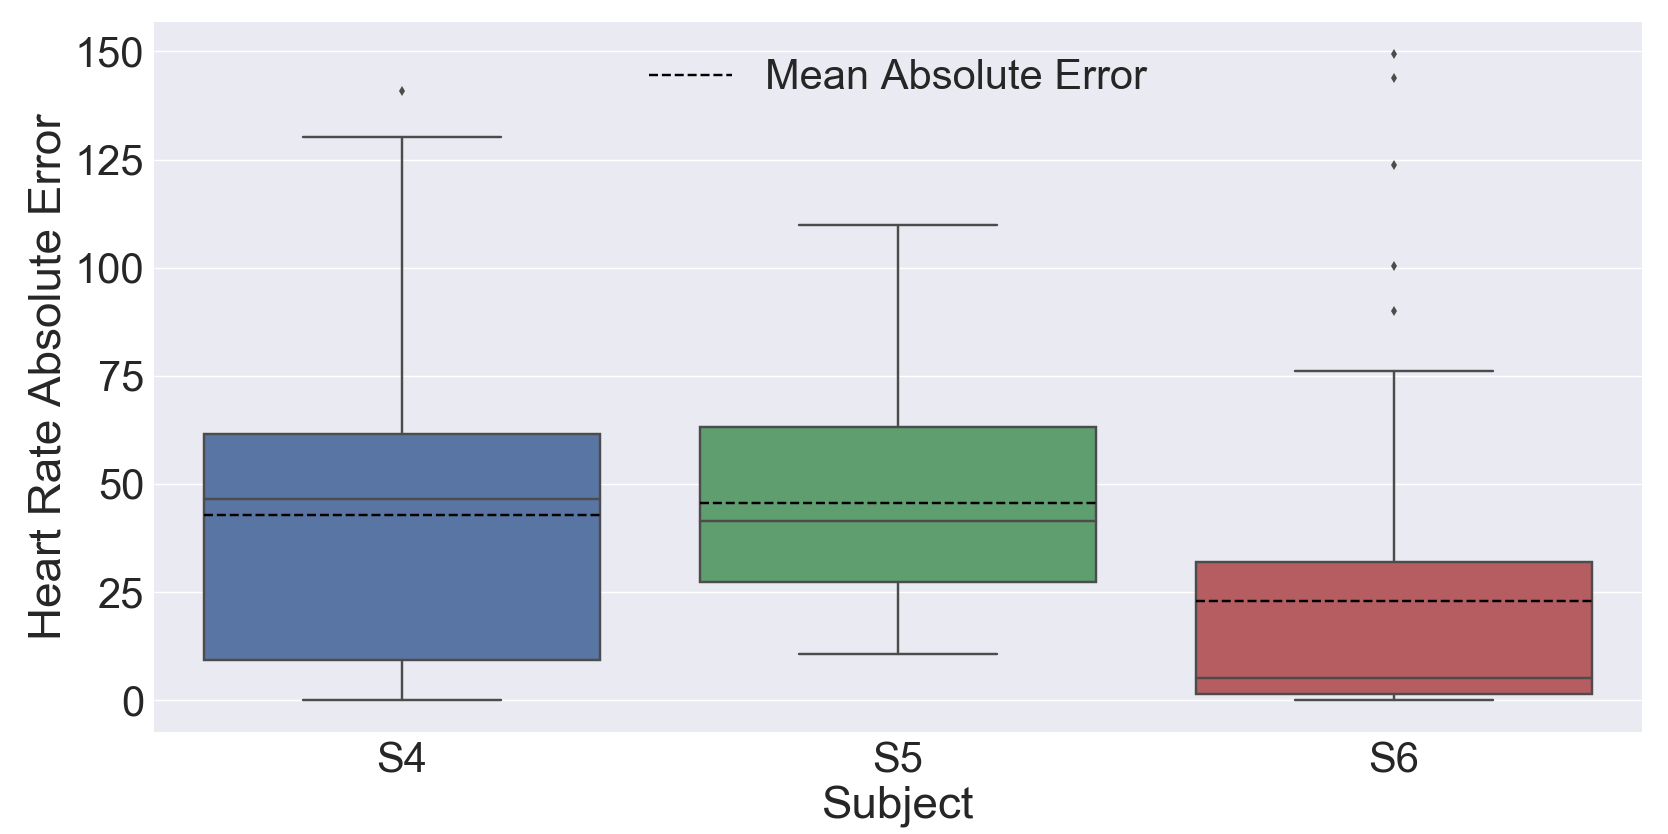
\includegraphics[width=0.85\textwidth]{box_h.png}
	\caption{Absolute Error of HR during stress test.}
	\label{figure:box_h}
\end{figure}

\begin{figure}[!h]
	\centering
	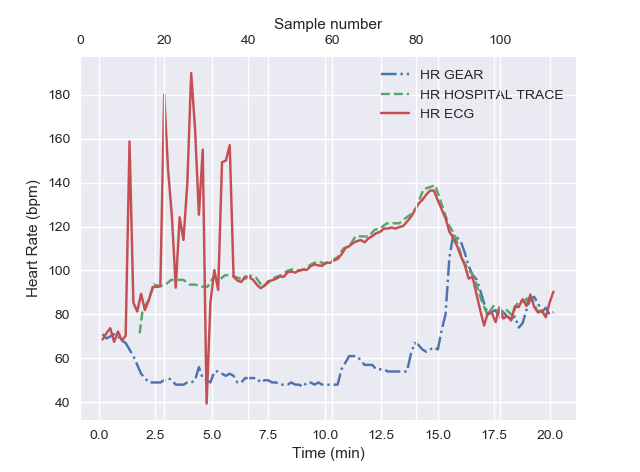
\includegraphics[width=0.85\textwidth]{HR_hospital.png}
	\caption{Example of HR curve obtained during stress test.}
	\label{figure:hr_hosp}
\end{figure}

\subsection{Discussion}

When observing the results obtained, the first conclusion that can be made is that the PPG signal collected with Samsung Gear S3 is very easily corrupted by motion artifacts. This corruption is present either during exercise or daily-life activities and even with very light movements, some corruption can be noticed. This means that very easily, the identification of systolic peaks in the signal cannot be made reliably, having a negative impact in the HR determination accuracy thus rendering this device unfit for pervasive monitoring in a medical context.

The main reasons for this low accuracy can be related with the sensor itself and also with the device as a whole. The sensor has only one green LED and one photodiode, while other sensors have two of each, with LEDs of different wavelengths. This apparent redundancy has a great impact as it allows for a different signal processing approach that can greatly improve the performance, while having only one wavelength means less information being collected, reducing the signal processing options. 

Concerning the weight, it must be taken into account that this is a very complex device that can perform endless tasks with native support for 3rd party apps. All these functionalities and capabilities make the device heavier and lager, thus, making it harder to keep comfortably and tightly secure to the wrist without it having its own dynamics. This is a problem as the relative movement between the sensor and the subject is the sole cause for movement artifacts in the signal. In addition the positioning of the sensor in an area with a relatively low SNR greatly increases the impact of motion artifacts. Also this device has the sensor at the same level of the watch back plate, whereas other devices place the sensor in an elevation of the back plate, which makes the sensor to be slightly pressed against the skin increasing SNR, and thus, accuracy. 

Due to poor quality PPG signal acquired, several algorithms were used in an attempt to get better HR estimates.
Algorithms used included adaptive filtering with and without Laguerre expansion \cite{adagibbs2005active,laguerrewood2006active}, signal separation by sparse signal reconstruction \cite{zhang2015joss,zhang2015troika} and onset detection \cite{bvponsetblazek2010multi}. A total of 8 algorithms were used to process the PPG and accelerometry data coming from S3 to produce estimates of HR. However, the results obtained using all this algorithms performed equally bad, or even worse, than Gear's algorithm and, for this reason, they were not considered. This clearly indicates that elevated error in Gear's HR estimations is probably related with a low quality signal and not with a poorly performing algorithm.

\FloatBarrier

\section{Heart Rate Estimation from ECG data}
\label{chapter:android_ecg_testing}

As a way of validating the algorithm described in \cref{chapter:android_ecg} running on the smartphone, that is being used to determine the HR from the ECG signal, a comparative analysis was made between the HR estimates based on the proposed algorithm and a standard one described in \cref{chapter:hr_ecg}.

The main difference between algorithms is that one is a very simplified RP detector running in the smartphone in real-time while the other runs off-line with no complexity restrictions.

\subsection{Methodology and Experimental Setup}

During E2, described in \cref{chapter:experiments}, ECG was collected by the chest band and was used to test the algorithm proposed in \cref{chapter:android_ecg}. At the same time, the raw signal was recorded and processed off-line by the standard algorithm. This allowed to isolate signal quality from the tests, as the same signal, divided in the same 10s windows was being processed by both algorithms and HR estimates were compared.

\FloatBarrier
\subsection{Results}

In \cref{figure:hr_android} the HR curves calculated by both algorithm can be seen. The calculations, for this particular subject, present an almost zero error, as the curves appear to be overlapping for almost all samples, and with minor deviations in a few points.

Looking at \cref{figure:erro_android} it can be noticed that observations made from \cref{figure:hr_android} are in agreement with error values for most subjects.

\begin{figure}[!h]
	\centering
	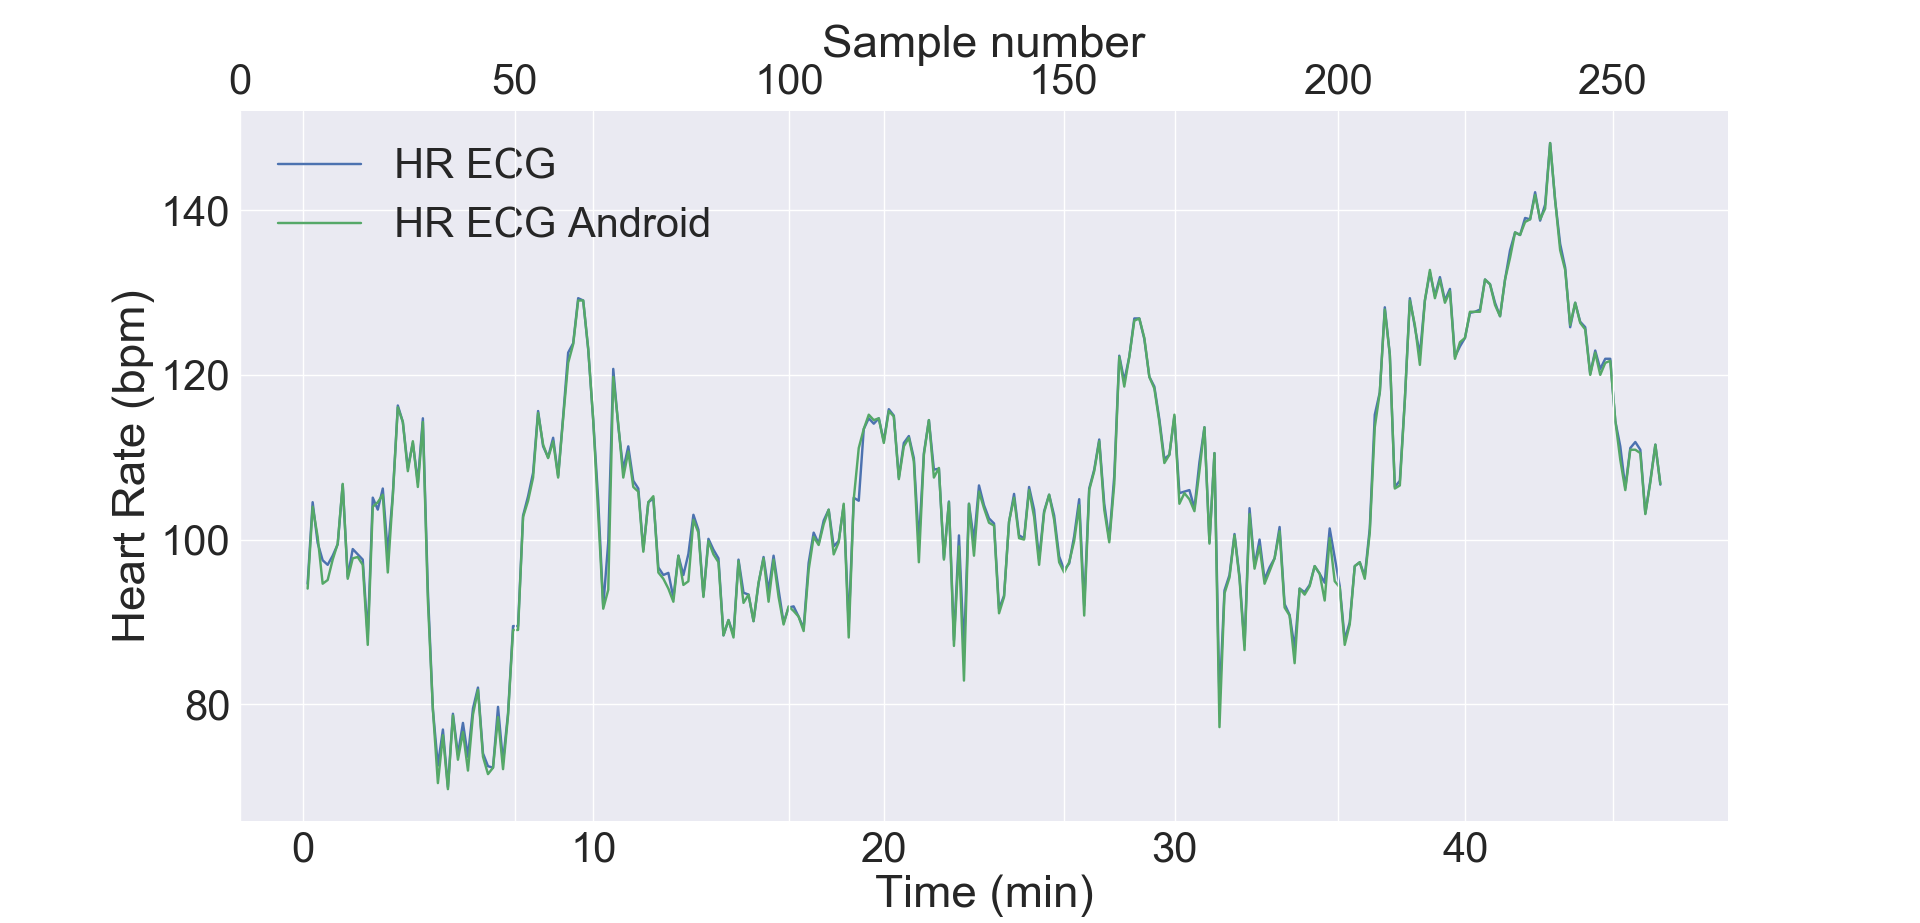
\includegraphics[width=0.85\textwidth]{hr-android-ecg.png}
	\caption{Error of android segmenter.}
	\label{figure:hr_android}
\end{figure}

\begin{figure}[!h]
	\centering
	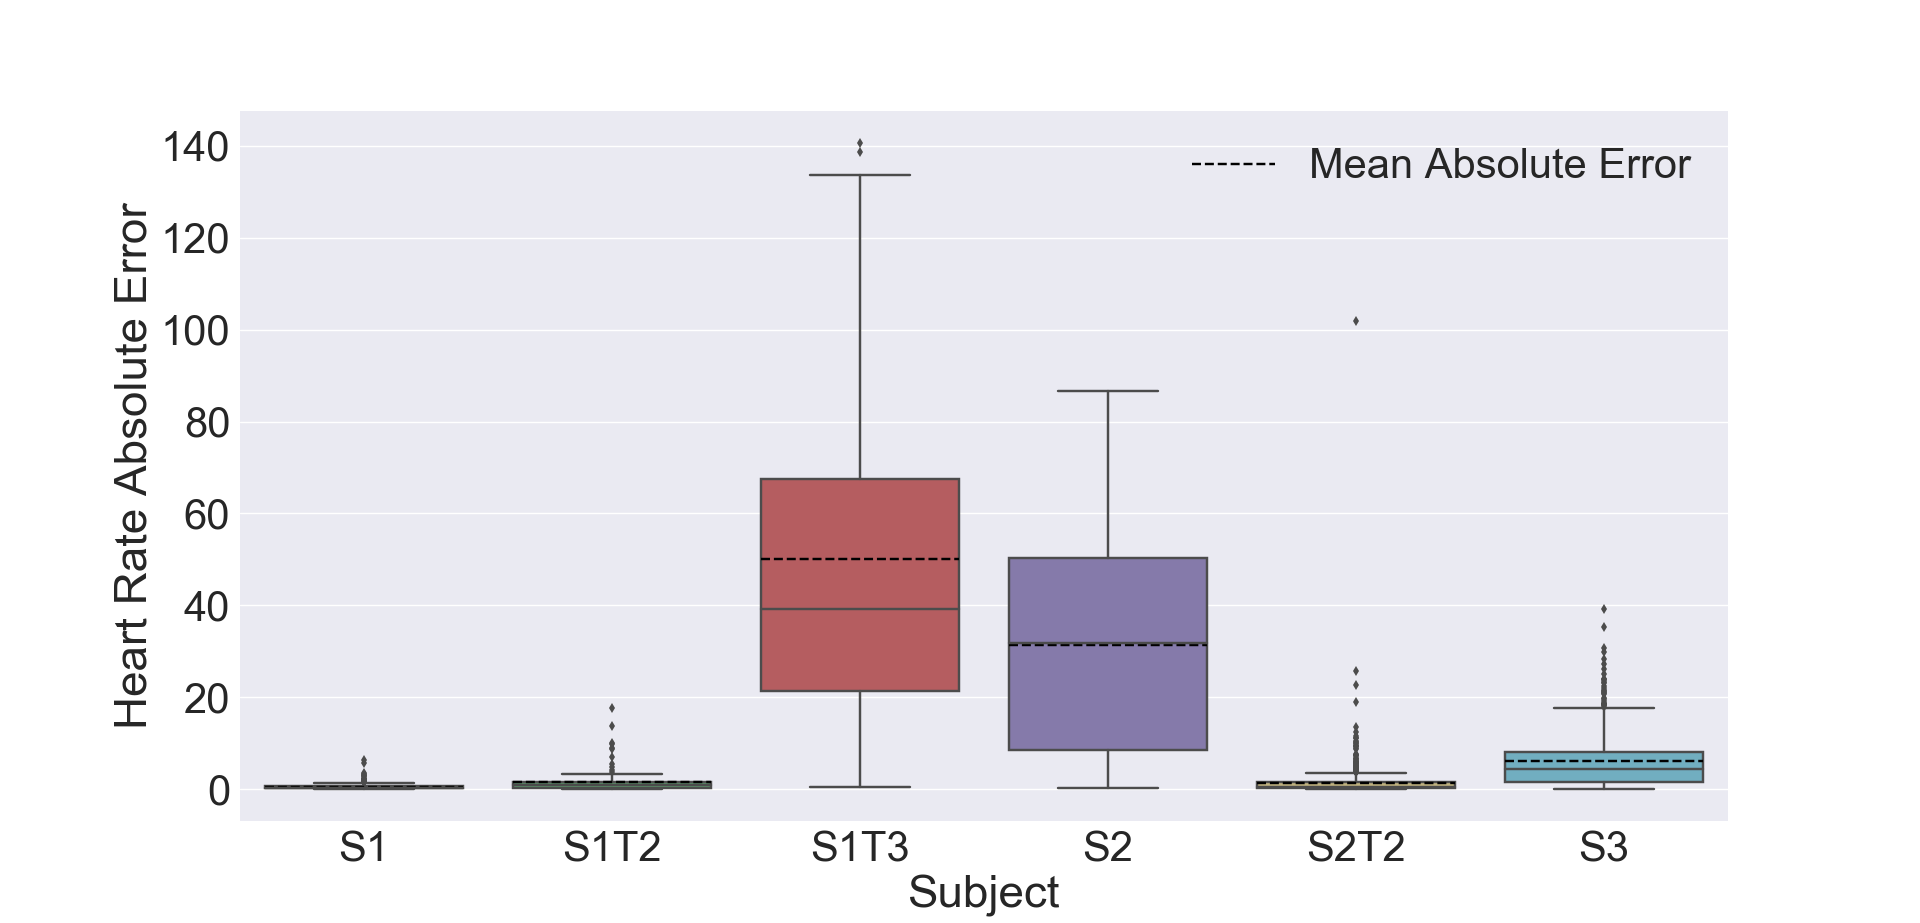
\includegraphics[width=0.85\textwidth]{erro-android-ecg.png}
	\caption{Error of android segmenter.}
	\label{figure:erro_android}
\end{figure}

\subsection{Discussion}

Analyzing \cref{figure:hr_android}, it can be noticed that HR estimation made using the proposed algorithm and the reference algoritm \cite{engzee} are rather small. This demonstrates that, even being computationally lightweight, it perform  well during daily-life tasks. Although BITalino produces a good quality ECG signal, when the wearer is moving, some artifacts are introduced, and even in this situation, HR estimates are reliable. This is confirmed by \cref{figure:erro_android}, where very small errors predominate with exception for two subjects S1T3 and S2, where Si denotes subject i and Tj denotes jth trial. In this particular pair of acquisitions, the increase of error is probably due to the introduction of motion artifacts in the ECG signal, as subjects reported to be exercising.

Besides motion artifacts, the other major weakness of this algorithm is chest band placement. This occurs due to the nature of the algorithm, as it is based in amplitude, it is expected of the R-peak to have an amplitude much larger than other signal features, which is only true for certain ECG electrodes placement. In case of a patient misplacing the chest band, it may be that signal morphology is altered leading to great errors in the HR estimation. However, with careful teaching of each patient on how to operate the system, this problem can be reduced (although not completely eliminated). To solve this problem a completely different algorithm would be needed, being, probably, much more elaborate and resource consuming.



%\begin{figure}[!h]
%	\centering
%	\makebox[\linewidth][c]{%
%		\begin{subfigure}[t]{0.55\textwidth}
%			\centering
%			\captionsetup{width=.75\linewidth}
%			\includegraphics[width=\textwidth]{hr-android-Andre.png}
%			\caption{Subject 1 HR}
%		\end{subfigure}%
%		\begin{subfigure}[t]{0.55\textwidth}
%			\centering
%			\captionsetup{width=.75\linewidth}
%			\includegraphics[width=\textwidth]{erro-android-Andre.png}
%			\caption{Subject 1 Absolute error and total accelerometry power}
%		\end{subfigure}%
%	}\\
%	\makebox[\linewidth][c]{%
%		\begin{subfigure}[t]{0.55\textwidth}
%			\centering
%			\captionsetup{width=.75\linewidth}
%			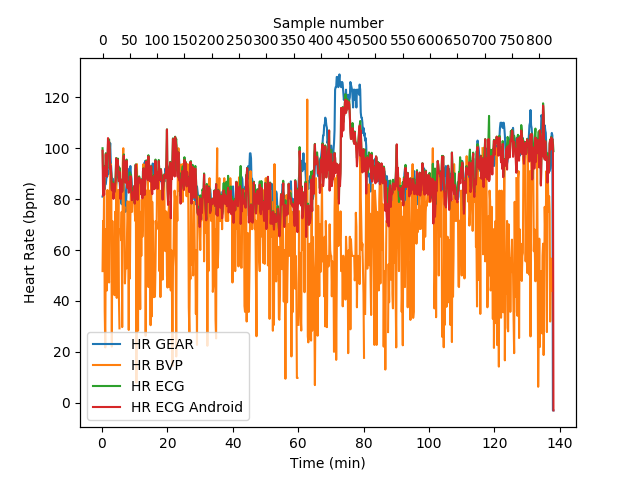
\includegraphics[width=\textwidth]{hr-android-Miguel.png}
%			\caption{Subject 2 HR}
%		\end{subfigure}%
%		\begin{subfigure}[t]{0.55\textwidth}
%			\centering
%			\captionsetup{width=.75\linewidth}
%			\includegraphics[width=\textwidth]{erro-android-Miguel.png}
%			\caption{Subject 2 Absolute error and total accelerometry power}
%		\end{subfigure}%
%	}\\
%	\makebox[\linewidth][c]{%
%		\begin{subfigure}[t]{0.55\textwidth}
%			\centering
%			\captionsetup{width=.75\linewidth}
%			\includegraphics[width=\textwidth]{hr-android-Andre-curto.png}
%			\caption{Subject 3 HR}
%		\end{subfigure}%
%		\begin{subfigure}[t]{0.55\textwidth}
%			\centering
%			\captionsetup{width=.75\linewidth}
%			\includegraphics[width=\textwidth]{erro-android-Andre-curto.png}
%			\caption{Subject 3 Absolute error and total accelerometry power}
%		\end{subfigure}	%
%	}\\
%	\caption{\textbf{Left:} Heart Rate determined from various methods: (blue) Gear's algorithm; (orange) using BVP data and an onset detector; (red) in the computer using a state-of-the-art algorithm; (green) the proposed real-time algorithm. \textbf{Right:} Heart Rate Absolute Error from each of the methods used and Accelerometry Energy}
%	\label{fig:hr-android}
%\end{figure}
%
%\begin{table}[h]
%	\centering
%	\caption{Root Mean Squared Error \cref{eq:rmse} from each of the subjects (S1, S2, S3) and the average RMS (AV) over the three subjects, when HR is calculated either from the raw BVP signal, by the Gear or with the proposed segmenter}
%	\label{table:error-android}
%	\begin{tabular}{c|c|c|c|c|c|c|}
%		\cline{2-7}
%		& S1    & S2    & S3  & S1 (2nd)  & S3 (2nd) & \textbf{AV}    \\ \hline
%		\multicolumn{1}{|c|}{HR Android} & 0.9  & 4.4  &  3.0  &  &   & \textbf{}  \\ \hline
%		\multicolumn{1}{|c|}{HR Gear}  & 13.1 & 9.7 &  18.0 &   &   & \textbf{} \\ \hline
%		\multicolumn{1}{|c|}{HR BVP} & 56.5 & 34.5  &  21.8 &   &    & \textbf{}  \\ \hline
%	\end{tabular}
%\end{table}


Overall, the algorithm performed very well, speacially when taking its simplicity into account. Robustness may be questionable when exercising, but for daily-life activities, it is very reliable, and improving the reliability would, probably, require a great increase in the computational burden of the algorithm, harming the smartphone's battery life and the general system's usability. % file "Thesis_Implementation.tex"
\cleardoublepage

%
\chapter{Evaluation of Accuracy in Heart Rate Determination using Samsung Gear S3 Smartwatch BVP data}

\section{Objective}

This experiment aims to conclude on the reliability of Samsung Gear Gear Smartwatch Photoplethysmography sensor (PPG) as a way to determine heart rate (HR).
In order to determine the accuracy of HR given by Gear, a BitAlino based chest-band was used, to acquire ECG simultaneously to the collection of PPG, and provide a ground-truth for heart rate. Besides Gear's HR calculation, an onset detection algorithm was also used to determine HR from PPG data.

\section{Experimental Procedure}

Three young subjects volunteered to this evaluation and data was collected in different situations from both ECG and PPG sensors:
\begin{description}[labelindent=\parindent]
	\item[--] 2 minutes resting, with the arm where the Gear was placed being completely still;
	\item[--] 5 minutes walking at a regular pace;
	\item[--] \(\sim\)2 hours where the subjects were told to behave like they normally would in their day-to-day life
\end{description}

\noindent

To guarantee consistency in results, the resting and walking experiments were repeated with two of the subjects for 5 and 10 minutes, respectively.

Heart rate was calculated in 10s windows using three different methods:
	
\begin{description}[labelindent=\parindent]
	\item[--] ECG signal was filtered and segmented in order to locate the R-peak and calculate HR. Filtering stage was composed of a median filter, a low-pass filter and a second median filter;
	\item[--] PPG signal was filtered, segmented and finally an onset detector was used to identify beats;
	\item[--] PPG was used by the Gear pre-implemented algorithm to internally produce a value of HR (the methods used to this are not known);
\end{description}

These methods were applied in each 10s window to allow an estimation of instantaneous HR, that is updated every 10s.

During all the experiments, 3axis accelerometry from the Gear was collected. This had the objective of determining if the increase in movement, induced a larger error in HR determination, by the introduction of motion artifacts (MA) in the PPG signal. From the raw accelerometry signal, the Total energy was calculated according with \Cref{eq:acc_energy}, to provide an heuristic on the "quantity of movement" at wrist level.

\begin{equation}
	E_{ACC}(n)= {{ACC}_{x}(n)}^{2}+{{ACC}_{y}(n)}^{2}+{{ACC}_{z}(n)}^{2}
	\label{eq:acc_energy}
\end{equation}


\FloatBarrier

\section{Results}

\subsection{Rest and walking}



\begin{figure}[!h]
	\centering
	\makebox[\linewidth][c]{%
		\begin{subfigure}[t]{0.55\textwidth}
			\centering
			\captionsetup{width=.75\linewidth}
			\includegraphics[width=\textwidth]{hr-andre-repouso.png}
			\caption{Heart Rate (Subject 1 resting)}
		\end{subfigure}%
		\begin{subfigure}[t]{0.55\textwidth}
			\centering
			\captionsetup{width=.75\linewidth}
			\includegraphics[width=\textwidth]{erro-andre-repouso.png}
			\caption{Absolute error and total accelerometry power (Subject 1 resting)}
		\end{subfigure}%
	}\\
	\makebox[\linewidth][c]{%
		\begin{subfigure}[t]{0.55\textwidth}
			\centering
			\captionsetup{width=.75\linewidth}
			\includegraphics[width=\textwidth]{hr-rita-repouso.png}
			\caption{Heart Rate (Subject 2 resting)}
		\end{subfigure}%
		\begin{subfigure}[t]{0.55\textwidth}
			\centering
			\captionsetup{width=.75\linewidth}
			\includegraphics[width=\textwidth]{erro-rita-repouso.png}
			\caption{Absolute error and total accelerometry power (Subject 2 resting)}
		\end{subfigure}%
	}\\
	\makebox[\linewidth][c]{%
		\begin{subfigure}[t]{0.55\textwidth}
			\centering
			\captionsetup{width=.75\linewidth}
			\includegraphics[width=\textwidth]{hr-miguel-repouso.png}
			\caption{Heart Rate (Subject 3 resting)}
		\end{subfigure}%
		\begin{subfigure}[t]{0.55\textwidth}
			\centering
			\captionsetup{width=.75\linewidth}
			\includegraphics[width=\textwidth]{erro-miguel-repouso.png}
			\caption{Absolute error and total accelerometry power (Subject 3 resting)}
		\end{subfigure}	%
	}\\
	\caption{HR determined using different methods and the erors associated}
	\label{fig:rest}
\end{figure}

\begin{figure}[!h]
	\centering
	\makebox[\linewidth][c]{%
		\begin{subfigure}[t]{0.55\textwidth}
			\centering
			\captionsetup{width=.75\linewidth}
			\includegraphics[width=\textwidth]{hr-andre-repouso-longo.png}
			\caption{Heart Rate (Repetition: Subject 1 resting)}
		\end{subfigure}%
		\begin{subfigure}[t]{0.55\textwidth}
			\centering
			\captionsetup{width=.75\linewidth}
			\includegraphics[width=\textwidth]{erro-andre-repouso-longo.png}
			\caption{Absolute error and total accelerometry error (Repetition: Subject 1 resting)}
		\end{subfigure}%
	}\\
	\makebox[\linewidth][c]{%
		\begin{subfigure}[t]{0.55\textwidth}
			\centering
			\captionsetup{width=.75\linewidth}
			\includegraphics[width=\textwidth]{hr-miguel-repouso-longo.png}
			\caption{Heart Rate (Repetition: Subject 1 resting)}
		\end{subfigure}%
		\begin{subfigure}[t]{0.55\textwidth}
			\centering
			\captionsetup{width=.75\linewidth}
			\includegraphics[width=\textwidth]{erro-miguel-repouso-longo.png}
			\caption{Absolute error and total accelerometry error (Repetition: Subject 3 resting)}
		\end{subfigure}%
	}\\	
	\caption{HR determined using different methods and the erors associated}
	\label{fig:rest2}
\end{figure}

\begin{figure}[!h]
	\centering
	\makebox[\linewidth][c]{%
		\begin{subfigure}[t]{0.55\textwidth}
			\centering
			\captionsetup{width=.75\linewidth}
			\includegraphics[width=\textwidth]{hr-andre-marcha.png}
			\caption{Heart Rate (Subject 1 walking)}
			\label{fig:walking-1}
		\end{subfigure}%
		\begin{subfigure}[t]{0.55\textwidth}
			\centering
			\captionsetup{width=.75\linewidth}
			\includegraphics[width=\textwidth]{erro-andre-marcha.png}
			\caption{Absolute error and total accelerometry error (Subject 1 walking)}
		\end{subfigure}%
	}\\
	\makebox[\linewidth][c]{%
		\begin{subfigure}[t]{0.55\textwidth}
			\centering
			\captionsetup{width=.75\linewidth}
			\includegraphics[width=\textwidth]{hr-rita-marcha.png}
			\caption{Heart Rate (Subject 2 walking)}
		\end{subfigure}%
		\begin{subfigure}[t]{0.55\textwidth}
			\centering
			\captionsetup{width=.75\linewidth}
			\includegraphics[width=\textwidth]{erro-rita-marcha.png}
			\caption{Absolute error and total accelerometry error (Subject 2 walking)}
		\end{subfigure}%
	}\\
	\makebox[\linewidth][c]{%
		\begin{subfigure}[t]{0.55\textwidth}
			\centering
			\captionsetup{width=.75\linewidth}
			\includegraphics[width=\textwidth]{hr-miguel-marcha.png}
			\caption{Heart Rate (Subject 3 walking)}
			\label{fig:walking-3}
		\end{subfigure}%
		\begin{subfigure}[t]{0.55\textwidth}
			\centering
			\captionsetup{width=.75\linewidth}
			\includegraphics[width=\textwidth]{erro-miguel-marcha.png}
			\caption{Absolute error and total accelerometry error (Subject 3 walking)}
		\end{subfigure}%
	}\\	
	\caption{Absolute Error calculated assuming HR from ECG as ground-truth.}
	\label{fig:walking}
\end{figure}

\begin{figure}[!h]
	\centering
	\makebox[\linewidth][c]{%
		\begin{subfigure}[t]{0.55\textwidth}
			\centering
			\captionsetup{width=.75\linewidth}
			\includegraphics[width=\textwidth]{hr-andre-marcha-longo.png}
			\caption{Heart Rate (Repetition: Subject 1 walking)}
		\end{subfigure}%
		\begin{subfigure}[t]{0.55\textwidth}
			\centering
			\captionsetup{width=.75\linewidth}
			\includegraphics[width=\textwidth]{erro-andre-marcha-longo.png}
			\caption{Absolute error and total accelerometry error (Repetition: Subject 1 walking)}
			\label{fig:walking2-2}
		\end{subfigure}%
	}\\
	\makebox[\linewidth][c]{%
		\begin{subfigure}[t]{0.55\textwidth}
			\centering
			\captionsetup{width=.75\linewidth}
			\includegraphics[width=\textwidth]{hr-miguel-marcha-longo.png}
			\caption{Heart Rate (Repetition: Subject 3 walking)}
		\end{subfigure}%
		\begin{subfigure}[t]{0.55\textwidth}
			\centering
			\captionsetup{width=.75\linewidth}
			\includegraphics[width=\textwidth]{erro-miguel-marcha-longo.png}
			\caption{Absolute error and total accelerometry error (Repetition: Subject 3 walking)}
		\end{subfigure}%
	}\\	
	\caption{Absolute Error calculated assuming HR from ECG as ground-truth.}
	\label{fig:walking2}
\end{figure}

\begin{equation}
	RMSE_{device}= \sqrt{\frac{1}{N}\sum\limits_{i=1}^N{(HR_{i_{device}}-HR_{i_{ECG}})}}
	\label{eq:rmse}
\end{equation}

\begin{table}[h]
	\centering
	\caption{Root Mean Squared Error \cref{eq:rmse} from each of the subjects (S1, S2, S3) and the average RMS (AV) over the three subjects, when HR is calculated either from the raw BVP signal or by the Gear}
	\label{table:error}
	\begin{tabular}{cc|c|c|c|c|c|c|}
		\cline{3-8}
		&      & S1    & S2    & S3  & S1 (2nd)  & S3 (2nd) & \textbf{AV}    \\ \hline
		\multicolumn{1}{|c|}{\multirow{2}{*}{Rest}} & BVP  & 2.1   & 1.6  & 1.2   & 1.4  & 1.5   & \textbf{1.6}  \\ \cline{2-8} 
		\multicolumn{1}{|c|}{}                      & Gear & 2.5  & 4.8  & 2.3   & 3.6  & 2.5  & \textbf{3.1}  \\ \hline
		\multicolumn{1}{|c|}{\multirow{2}{*}{Walking}} & BVP  & 42.9 & 30.7 & 33.3  & 42.3  & 37.9  & \textbf{46} \\ \cline{2-8} 
		\multicolumn{1}{|c|}{}                      & Gear & 14.0 & 4.3  & 7.4  & 41.12  &  5.2  & \textbf{36}  \\ \hline
	\end{tabular}
\end{table}

Analyzing the plots in \Cref{fig:rest,fig:rest2,fig:walking,fig:walking2}, it is easy to notice that the error in determining the HR while walking is far larger than during rest, which is made clear by the RMS error values in \Cref{table:error}. 

Another conclusion is that the calculation made with the onset detector, although working slightly better in rest, is much worse when the subject is walking. And despite Gear's calculation being more precise than the latter at rest state, there is still a non-negligible error in Gear's automatic calculation. This error becomes significantly worse when there are periods of maintained activity, as can be seen in \Cref{fig:walking2-2}, where the subject's accelerometry energy is elevated during the entire experiment, and the MA induced in BVP signal, lead to a very large error in HR determination.


\FloatBarrier
\pagebreak

\subsection{Event Detection}

\begin{figure}[!h]
	\centering
	\makebox[\linewidth][c]{%
		\begin{subfigure}[t]{0.55\textwidth}
			\centering
			\captionsetup{width=.75\linewidth}
			\includegraphics[width=\textwidth]{repouso-ecg.png}
			\caption{Segment of ECG signal with the detected R-peaks during rest}
		\end{subfigure}%
		\begin{subfigure}[t]{0.55\textwidth}
			\centering
			\captionsetup{width=.75\linewidth}
			\includegraphics[width=\textwidth]{repouso-bvp.png}
			\caption{Segment of BVP signal with the detected onsets during rest}
		\end{subfigure}%
	}\\
	\makebox[\linewidth][c]{%
		\begin{subfigure}[t]{0.55\textwidth}
			\centering
			\captionsetup{width=.75\linewidth}
			\includegraphics[width=\textwidth]{marcha-ecg.png}
			\caption{Segment of ECG signal with the detected R-peaks while walking}
		\end{subfigure}%
		\begin{subfigure}[t]{0.55\textwidth}
			\centering
			\captionsetup{width=.75\linewidth}
			\includegraphics[width=\textwidth]{marcha-bvp.png}
			\caption{Segment of BVP signal with the detected onsets while walking}
		\end{subfigure}%
	}\\
	\caption{Raw ECG and BVP signals and the respective events detected when resting and walking}
	\label{fig:events}
\end{figure}


\begin{table}[!h]
	\centering
	\caption{Number of detected beats in each activity and ratio between $ \# $beats in ECG and BVP}
	\label{table:beats}
	\begin{tabular}{cc|c|c|c|c|}
		\cline{3-6}
		&                & S1            & S2            & S3            & AV            \\ \hline
		\multicolumn{1}{|c|}{\multirow{3}{*}{Rest}}    & BVP            & 137           & 145           & 142           & 141           \\ \cline{2-6} 
		\multicolumn{1}{|c|}{}                         & ECG           & 137           & 154           & 145           & 145           \\ \cline{2-6} 
		\multicolumn{1}{|c|}{}                         & \textbf{Ratio} & \textbf{1}    & \textbf{0.94} & \textbf{0.97} & \textbf{0.91} \\ \hline
		\multicolumn{1}{|c|}{\multirow{3}{*}{Walking}} & ECG            & 127           & 191           & 152           & 157           \\ \cline{2-6} 
		\multicolumn{1}{|c|}{}                         & Gear           & 402           & 387           & 348           & 379           \\ \cline{2-6} 
		\multicolumn{1}{|c|}{}                         & \textbf{Ratio} & \textbf{0.32} & \textbf{0.5}  & \textbf{0.44} & \textbf{0.42} \\ \hline
	\end{tabular}
\end{table}


As it can be observed in \Cref{fig:events} the detection of events while in rest works very well for both the chest-band ECG and the wrist BVP. 

On the other hand, when subject moves, this detection is much harder due to MA corrupting the BVP signal and thus, making the task of detecting the beat onset very hard. This does not occur with the ECG signal since the chest-band is far less sensible to artifacts, having a higher SNR.

These conclusions are corroborated by \Cref{table:beats} where a clear difference in detection performance is obvious. Near 100\% of beats are detected in the BVP signal when resting, whereas, the percentage drops to less than a half when walking. This confirms the poor performance of the onset detection algorithm in the presence of MA.

In \Cref{fig:zoom}, examples of raw signal windows used to calculate HR can be seen, each illustrating a different situation. 

In \Cref{fig:zoom1} is the signal used to calculate sample 15 of the experiment where S3 was walking. As \Cref{fig:walking-3} shows, in this instance HR has a rapid increase, while Gear's estimation remains almost constant, demonstrating Gear's poor ability to deal with rapid changes in HR. 

In \Cref{fig:zoom2}, a very different situation is depicted. Here Gear's error is fairly small and BVP error is very big. This figure contains the raw signal used to calculate the sample nr 2 in \Cref{fig:walking-3}. Here the "quantity of movement" detected was relatively low and HR was fairly constant. This demonstrates that, when the subject is not moving very much, Gear's calculation is relatively accurate, which is not true for onset detection algorithm that has a large error with the slightest movement.

Finally \Cref{fig:zoom3} corresponds to a situation with large error in both methods. This is due, again, to the introduction of MA in the BVP signal.

An observation that can be made from all this examples, is that a peak in accelerometry energy, induces invariably a disruption in the BVP signal, that is amplified by the filtration used. This supports the hypothesis of high correlation level existing between movement, and deterioration of SNR in BVP.



\begin{figure}[!h]
	\centering
	\begin{subfigure}[t]{0.5\textwidth}
		\centering
		\captionsetup{width=.8\linewidth}
		\includegraphics[width=\textwidth]{zoom-miguel-marcha-15.png}
		\caption{Raw signal used to determine sample nr 15 of Subject 3 heart rate while walking. BVP error: 57.5bpm; Gear error: 15.8bpm}
		\label{fig:zoom1}
	\end{subfigure}%
	\begin{subfigure}[t]{0.5\textwidth}
		\centering
		\captionsetup{width=.8\linewidth}
		\includegraphics[width=\textwidth]{zoom-miguel-marcha-2.png}
		\caption{Raw signal used to determine sample nr 2 of Subject 3 heart rate while walking. BVP error: 60.4bpm; Gear error: 0.85bpm}
		\label{fig:zoom2}
	\end{subfigure}%
	\vskip 8pt
	\begin{subfigure}[t]{0.5\textwidth}
		\centering
		\captionsetup{width=.8\linewidth}
		\includegraphics[width=\textwidth]{zoom-andre-marcha-1.png}
		\caption{Raw signal used to determine sample nr 1 of Subject 1 heart rate while walking. BVP error: 54.9bpm; Gear error: 24.3bpm}
		\label{fig:zoom3}
	\end{subfigure}%
	
	\caption{Examples of raw signal windows used to calculate heart rate samples and the simultaneously acquired accelerometry}
	\label{fig:zoom}
\end{figure}


\FloatBarrier
\pagebreak

\subsection{"Real life" case}


\begin{figure}[!h]
	\centering
	\makebox[\linewidth][c]{%
	\begin{subfigure}[t]{0.55\textwidth}
		\centering
		\includegraphics[width=\textwidth]{hr-andre-continuo.png}
		\caption{Subject 1 HR}
	\end{subfigure}%
	\begin{subfigure}[t]{0.55\textwidth}
		\centering
		\includegraphics[width=\textwidth]{erro-andre-continuo.png}
		\caption{Subject 1 Absolute Error and Accelerometry Energy}
		\label{fig:real-acc1}
	\end{subfigure}%
	}\\
	\makebox[\linewidth][c]{%
	\begin{subfigure}{0.55\textwidth}
		\centering
		\includegraphics[width=\textwidth]{hr-rita-continuo.png}
		\caption{Subject 2 HR}
	\end{subfigure}%	
	\begin{subfigure}{0.55\textwidth}
		\centering
		\includegraphics[width=\textwidth]{erro-rita-continuo.png}
		\caption{Subject 2 Absolute Error and Accelerometry Energy}
		\label{fig:real-acc2}
	\end{subfigure}%
	}\\
	\caption{HR and squared error during a segment of the subjects' daily life}
	\label{fig:real}
\end{figure}

\begin{table}[!h]
	\label{table:real}
	\centering
	\caption{Root Mean Squared error from each of the subjects (S1, S2, S3) and the average RMS (AV) when HR is calculatd from the raw BVP signal and by the Gear}
	\begin{tabular}{l|l|l|l|l|}
		\cline{2-5}
		& S1    & S2 & S3    & \textbf{AV}    \\ \hline
		\multicolumn{1}{|l|}{BVP}  & 17.39 & -- & 24.51 & \textbf{20.95} \\ \hline
		\multicolumn{1}{|l|}{Gear} & 31.23 & -- & 26.99 & \textbf{29.11} \\ \hline
	\end{tabular}
\end{table}

\FloatBarrier


It is possible to observe that the determination of HR during the subjects' daily-life presents a considerable amount of error. The HR instantaneous error reached a very high value of more than 40bpm. On top of this high instantaneous error, the average error is also relatively high, reaching 16bpm, indicating the calculation is untrustworthy during most of the acquisition time.

On top of this, it is possible to observe in \Cref{fig:real-acc1} and \ref{fig:real-acc2}, that an increase in movement, (indicated by the larger accelerometry energy) is associated with an increase in Gear's error. This is visible in \Cref{fig:real-acc1} where a region of significant and maintained increase in error, coincides with a period of higher accelerometry energy.

Also in \Cref{fig:real-acc2} the subject kept a high level of activity and the error was considerable. Demonstrating a clear relation between "quantity of movement" and error. Being the only explanation for this, the high corruption of the BVP signal, by the introduction of MA.

\section{Conclusions}



The results of this analysis, clearly indicate that the Gear's automatic calculations and the BVP onset detection are not enough to guarantee accuracy in HR determination for long term studies, especially if the subject is moving. The main reason for this methods' failure is the poor capacity to deal with motion artifacts, conclusion that is supported by the relatively small error when the subject is resting, that increases dramatically when in movement.


A possible strategy to deal with this problem, may be, using an algorithm that takes accelerometry into account and tries to remove movement artifacts and get a denoised BVP signal, with better SNR.
 % file "Thesis_Implementation.tex"
%\cleardoublepage
%
%
\chapter{System Testing during Stress Test}

\section{Overview}

Two patients wore the system while performing a stress test on the treadmill following the modified Bruce protocol. Information about heart rate and motion was recorded by the proposed system and hospital equipment.

The objective of this experiment was to compare the reliability of various sources of HR and METs values.

During the experiment, patient wore both, the proposed system and hospital's equipment, which caused some problems with electrode placement and, in some periods, lead to the loss of ECG data due to a bad contact between the chest band and the skin.

\FloatBarrier
\section{Results}

Data from hospital equipment is available from two sources, in files with a sampling rate of 1 sample/min or in the form of plots saved as images. From this images, data was traced with higher sampling rate, although this manual tracing, inevitably, introduced some error to the values recovered.

\begin{figure}[!h]
	\centering
	\makebox[\linewidth][c]{%
		\begin{subfigure}[t]{0.55\textwidth}
			\centering
			\captionsetup{width=.75\linewidth}
			\includegraphics[width=\textwidth]{hr-android-4-4.png}
			\caption{Subject 1}
		\end{subfigure}%
		\begin{subfigure}[t]{0.55\textwidth}
			\centering
			\captionsetup{width=.75\linewidth}
			\includegraphics[width=\textwidth]{hr-android-5-5.png}
			\caption{Subject 2}
		\end{subfigure}%
	}\\

	\caption{Heart Rate calculated from various sources: (blue) Gear's algorithm; (orange) Values returned from hospital equipment; (green) Values traced from plot printed by hospital equipment; (red) State of the art ECG segmenter; (purple) Simplified segmenter implemented in phone}

	\makebox[\linewidth][c]{%
		\begin{subfigure}[t]{0.55\textwidth}
			\centering
			\captionsetup{width=.75\linewidth}
			\includegraphics[width=\textwidth]{erro-android-4-4.png}
			\caption{Subject 1}
			\label{fig:hosp-hr-4}
		\end{subfigure}%
		\begin{subfigure}[t]{0.55\textwidth}
			\centering
			\captionsetup{width=.75\linewidth}
			\includegraphics[width=\textwidth]{erro-android-5-5.png}
			\caption{Subject 2}
			\label{fig:hosp-hr-5}
		\end{subfigure}%
	}\\

	\caption{Error from the various methods using state of the art segmenter as ground truth (hospital data was not compared due to different sampling rate)}

	\makebox[\linewidth][c]{%
		\begin{subfigure}[t]{0.55\textwidth}
			\centering
			\captionsetup{width=.75\linewidth}
			\includegraphics[width=\textwidth]{mets-android-4-4.png}
			\caption{Subject 1}
		\end{subfigure}%
		\begin{subfigure}[t]{0.55\textwidth}
			\centering
			\captionsetup{width=.75\linewidth}
			\includegraphics[width=\textwidth]{mets-android-5-5.png}
			\caption{Subject 2}
		\end{subfigure}	%
	}\\

	\caption{METs determined from different sources:  (blue) Gear's accelerometer; (orange) Values returned from hospital equipment; (green) Values traced from plot printed by hospital equipment; (red) Phone accelerometer}

	\label{fig:hosp}
\end{figure}

%RAW
\begin{figure}[!h]
	\centering
	\makebox[\linewidth][c]{%
		\begin{subfigure}[t]{0.55\textwidth}
			\centering
			\captionsetup{width=.75\linewidth}
			\includegraphics[width=\textwidth]{ecg-4-4.png}
			\caption{Subject 1}
			\label{fig:hosp-raw-4}
		\end{subfigure}%
		\begin{subfigure}[t]{0.55\textwidth}
			\centering
			\captionsetup{width=.75\linewidth}
			\includegraphics[width=\textwidth]{ecg-5-5.png}
			\caption{Subject 2}
			\label{fig:hosp-raw-5}
		\end{subfigure}%
	}\\
	
	\caption{Raw ECG acquired by the chest band when processed by android segmenter (blue) and by a state of the art algorithm (orange)}
	
	\makebox[\linewidth][c]{%
		\begin{subfigure}[t]{0.55\textwidth}
			\centering
			\captionsetup{width=.75\linewidth}
			\includegraphics[width=\textwidth]{ecg-4-4-good.png}
			\caption{Subject 1 - ECG segment used to calculate sample nr 50 of HR (\cref{fig:hosp-hr-4})}
		\end{subfigure}%
		\begin{subfigure}[t]{0.55\textwidth}
			\centering
			\captionsetup{width=.75\linewidth}
			\includegraphics[width=\textwidth]{ecg-5-5-good.png}
			\caption{Subject 2 - ECG segment used to calculate sample nr 43 of HR (\cref{fig:hosp-hr-5})}
		\end{subfigure}%
	}\\

	\caption{Example of ECG segments used to calculate HR with small error}
	
	\makebox[\linewidth][c]{%
		\begin{subfigure}[t]{0.55\textwidth}
			\centering
			\captionsetup{width=.75\linewidth}
			\includegraphics[width=\textwidth]{ecg-4-4-bad.png}
			\caption{Subject 1 - ECG segment used to calculate sample nr 25 of HR (\cref{fig:hosp-hr-4})}
		\end{subfigure}%
		\begin{subfigure}[t]{0.55\textwidth}
			\centering
			\captionsetup{width=.75\linewidth}
			\includegraphics[width=\textwidth]{ecg-5-5-bad.png}	
			\caption{Subject 2 - ECG segment used to calculate sample nr 16 of HR (\cref{fig:hosp-hr-5})}
			\label{fig:hosp-raw-5-bom}
		\end{subfigure}	%
	}\\

	\caption{Example of ECG segments used to calculate HR with big error}
		
	\label{fig:hosp-raw}
\end{figure}


\FloatBarrier
\section{Conclusions}

As can be seen in \cref{fig:hosp-raw-5-bom} even when android and the state of the art algorithm detect the same R-peaks, which should indicate both are correct, the HR value obtained still is very different from the one returned by the hospital's equipment. This could indicate that ECG electrode placement was interfering with the ECG acquisition by the chest band. This hypothesis is supported by the fact that during approximately half of the experiment with subject 2, no ECG was acquired as can be seen in 	\cref{fig:hosp-raw-5}.

For Subject 1, although the electrode placement was still a problem, the ECG signal had good quality the majority of the time, allowing the algorithms to produce good results.

Regarding METs calculation, the results had significant error. This can be caused by several factors. One could be having subjects walking in a treadmill, which presents a fairly different accelerometer compared to really walking. 
%Another reason could be the calculation of METs by the hospital equipment that is(?) an estimation and not a measured value, this could introduce error as this estimation could be biased and not correspond to reality.


 % file "Thesis_Implementation.tex"
%\cleardoublepage

%%%%%%%%%%%%%%%%%%%%%%%%%%%%%%%%%%%%%%%%%%%%%%%%%%%%%%%%%%%%%%%%%%%%%%%%%
%                                                                      %
%     File: Thesis_Results.tex                                         %
%     Tex Master: Thesis.tex                                           %
%                                                                      %
%     Author: Andre C. Marta                                           %
%     Last modified :  2 Jul 2015                                      %
%                                                                      %
%%%%%%%%%%%%%%%%%%%%%%%%%%%%%%%%%%%%%%%%%%%%%%%%%%%%%%%%%%%%%%%%%%%%%%%%

\chapter{Results}
\label{chapter:results}

Insert your chapter material here...


%%%%%%%%%%%%%%%%%%%%%%%%%%%%%%%%%%%%%%%%%%%%%%%%%%%%%%%%%%%%%%%%%%%%%%%%
\section{Problem Description}
\label{section:problem}

Description of the baseline problem...


%%%%%%%%%%%%%%%%%%%%%%%%%%%%%%%%%%%%%%%%%%%%%%%%%%%%%%%%%%%%%%%%%%%%%%%%
\section{Baseline Solution}
\label{section:baseline}

Analysis of the baseline solution...


%%%%%%%%%%%%%%%%%%%%%%%%%%%%%%%%%%%%%%%%%%%%%%%%%%%%%%%%%%%%%%%%%%%%%%%%
\section{Enhanced Solution}
\label{section:enhanced}

Quest for the optimal solution...


% ----------------------------------------------------------------------
\subsection{Figures}
\label{subsection:figures}

Insert your section material and possibly a few figures...

Make sure all figures presented are referenced in the text!


% ----------------------------------------------------------------------
\subsubsection{Images}
\label{subsection:images}

\begin{figure}[!htb]
  \centering
  \includegraphics[width=0.25\textwidth]{Figures/Airbus_A350.jpg}
  \caption[Caption for figure in TOC.]{Caption for figure.}
  \label{fig:airbus1}
\end{figure}



By default, the supported file types are {\it .png,.pdf,.jpg,.mps,.jpeg,.PNG,.PDF,.JPG,.JPEG}.

See \url{http://mactex-wiki.tug.org/wiki/index.php/Graphics_inclusion} for adding support to other extensions.


% ----------------------------------------------------------------------
\subsubsection{Drawings}
\label{subsection:drawings}

Insert your subsection material and for instance a few drawings...

The schematic illustrated in Fig.~\ref{fig:algorithm} can represent some sort of algorithm.

\begin{figure}[!htb]
  \centering
  \scriptsize
%  \footnotesize 
%  \small
  \setlength{\unitlength}{0.9cm}
  \begin{picture}(8.5,6)
    \linethickness{0.3mm}

    \put(3,6){\vector(0,-1){1}}
    \put(3.5,5.4){$\bf \alpha$}
    \put(3,4.5){\oval(6,1){}}
    %\put(0,4){\framebox(6,1){}}
    \put(0.3,4.4){Grid Generation: \quad ${\bf x} = {\bf x}\left({\bf \alpha}\right)$}

    \put(3,4){\vector(0,-1){1}}
    \put(3.5,3.4){$\bf x$}
    \put(3,2.5){\oval(6,1){}}
    %\put(0,2){\framebox(6,1){}}
    \put(0.3,2.4){Flow Solver: \quad ${\cal R}\left({\bf x},{\bf q}\left({\bf x}\right)\right) = 0$}

    \put(6.0,2.5){\vector(1,0){1}}
    \put(6.4,3){$Y_1$}

    \put(3,2){\vector(0,-1){1}}
    \put(3.5,1.4){$\bf q$}
    \put(3,0.5){\oval(6,1){}}
    %\put(0,0){\framebox(6,1){}}
    \put(0.3,0.4){Structural Solver: \quad ${\cal M}\left({\bf x},{\bf q}\left({\bf x}\right)\right) = 0$}

    \put(6.0,0.5){\vector(1,0){1}}
    \put(6.4,1){$Y_2$}

    %\put(7.8,2.5){\oval(1.6,5){}}
    \put(7.0,0){\framebox(1.6,5){}}
    \put(7.1,2.5){Optimizer}
    \put(7.8,5){\line(0,1){1}}
    \put(7.8,6){\line(-1,0){4.8}}
  \end{picture}
  \caption{Schematic of some algorithm.}
  \label{fig:algorithm}
\end{figure}


% ----------------------------------------------------------------------
\subsection{Equations}
\label{subsection:equations}

Equations can be inserted in different ways.

The simplest way is in a separate line like this

\begin{equation}
  \frac{{\rm d} q_{ijk}}{{\rm d} t} + {\cal R}_{ijk}({\bf q}) = 0 \,.
\label{eq:ode}
\end{equation}

If the equation is to be embedded in the text. One can do it like this ${\partial {\cal R}}/{\partial {\bf q}}=0$.

It may also be split in different lines like this

\begin{eqnarray}
  {\rm Minimize}   && Y({\bf \alpha},{\bf q}({\bf \alpha}))            \nonumber           \\
  {\rm w.r.t.}     && {\bf \alpha} \,,                                 \label{eq:minimize} \\
  {\rm subject~to} && {\cal R}({\bf \alpha},{\bf q}({\bf \alpha})) = 0 \nonumber           \\
                   &&       C ({\bf \alpha},{\bf q}({\bf \alpha})) = 0 \,. \nonumber
\end{eqnarray}

It is also possible to use subequations. Equations~\ref{eq:continuity}, \ref{eq:momentum} and \ref{eq:energy} form the Naver--Stokes equations~\ref{eq:NavierStokes}.

\begin{subequations}
    \begin{equation}
    \frac{\partial \rho}{\partial t} + \frac{\partial}{\partial x_j}\left( \rho u_j \right) = 0 \,,
    \label{eq:continuity}
    \end{equation}
    \begin{equation}
    \frac{\partial}{\partial t}\left( \rho u_i \right) + \frac{\partial}{\partial x_j} \left( \rho u_i u_j + p \delta_{ij} - \tau_{ji} \right) = 0, \quad i=1,2,3 \,,
    \label{eq:momentum}
    \end{equation}
    \begin{equation}
        \frac{\partial}{\partial t}\left( \rho E \right) + \frac{\partial}{\partial x_j} \left( \rho E u_j + p u_j - u_i \tau_{ij} + q_j \right) = 0 \,.
    \label{eq:energy}
    \end{equation}
\label{eq:NavierStokes}%
\end{subequations}


% ----------------------------------------------------------------------
\subsection{Tables}
\label{section:tables}

Insert your subsection material and for instance a few tables...

Make sure all tables presented are referenced in the text!

Follow some guidelines when making tables:

\begin{itemize}
  \item Avoid vertical lines
  \item Avoid “boxing up” cells, usually 3 horizontal lines are enough: above, below, and after heading
  \item Avoid double horizontal lines
  \item Add enough space between rows
\end{itemize}

\begin{table}[!htb]
  \renewcommand{\arraystretch}{1.2} % more space between rows
  \centering
  \begin{tabular}{lccc}
    \toprule
    Model           & $C_L$ & $C_D$ & $C_{M y}$ \\
    \midrule
    Euler           & 0.083 & 0.021 & -0.110    \\
    Navier--Stokes  & 0.078 & 0.023 & -0.101    \\
    \bottomrule
  \end{tabular}
  \caption[Table caption shown in TOC.]{Table caption.}
  \label{tab:aeroCoeff}
\end{table}

Make reference to Table \ref{tab:aeroCoeff}.

Tables \ref{tab:memory} and \ref{tab:multipleColumns} are examples of tables with merging columns:

\begin{table}[!htb]
  \renewcommand{\arraystretch}{1.2} % more space between rows
  \centering
  \begin{tabular}[]{lrr}
    \toprule
                & \multicolumn{2}{c}{\underline{Virtual memory [MB]}} \\
                & Euler       & Navier--Stokes \\
    \midrule
      Wing only &  1,000      &    2,000       \\
      Aircraft  &  5,000      &   10,000       \\
      (ratio)   & $5.0\times$ & $5.0\times$    \\
    \bottomrule
  \end{tabular}
  \caption{Memory usage comparison (in MB).}
  \label{tab:memory}
\end{table}

\begin{table}[!htb]
  \centering
  \renewcommand{\arraystretch}{1.2} % more space between rows
  \begin{tabular}{@{}rrrrcrrr@{}} % remove space to the vertical edges @{}...@{}
    \toprule
      & \multicolumn{3}{c}{$w = 2$} & \phantom{abc} & \multicolumn{3}{c}{$w = 4$} \\
    \cmidrule{2-4}
    \cmidrule{6-8}
      & $t=0$ & $t=1$ & $t=2$ && $t=0$ & $t=1$ & $t=2$ \\
    \midrule
      $dir=1$
      \\
      $c$ &  0.07 &  0.16 &  0.29 &&  0.36 &  0.71 &   3.18 \\
      $c$ & -0.86 & 50.04 &  5.93 && -9.07 & 29.09 &  46.21 \\
      $c$ & 14.27 &-50.96 &-14.27 && 12.22 &-63.54 &-381.09 \\
      $dir=0$
      \\
      $c$ &  0.03 &  1.24 &  0.21 &&  0.35 & -0.27 &  2.14 \\
      $c$ &-17.90 &-37.11 &  8.85 &&-30.73 & -9.59 & -3.00 \\
      $c$ &105.55 & 23.11 &-94.73 &&100.24 & 41.27 &-25.73 \\
    \bottomrule
  \end{tabular}
  \caption{Another table caption.}
  \label{tab:multipleColumns}
\end{table}

An example with merging rows can be seen in Tab.\ref{tab:multipleRows}.

\begin{table}[!htb]
  \renewcommand{\arraystretch}{1.2} % more space between rows
  \centering
  \begin{tabular}{ccccc}
    \toprule
      \multirow{2}{*}{ABC} & \multicolumn{4}{c}{header} \\
      \cmidrule{2-5} & 1.1 & 2.2 & 3.3 & 4.4 \\
    \midrule
      \multirow{2}{*}{IJK} & \multicolumn{2}{c}{\multirow{2}{*}{group}} & 0.5 & 0.6 \\
      \cmidrule{4-5}       & \multicolumn{2}{c}{}                       & 0.7 & 1.2 \\
    \bottomrule
  \end{tabular}
  \caption{Yet another table caption.}
  \label{tab:multipleRows}
\end{table}

If the table has too many columns, it can be scaled to fit the text widht, as in Tab.\ref{tab:scale}.
\begin{table}[!htb]
  \renewcommand{\arraystretch}{1.2} % more space between rows
  \centering
  \resizebox*{\textwidth}{!}{%
    \begin{tabular}[]{lcccccccccc}
      \toprule
        Variable &  a  &  b  &  c  &  d  &  e  &  f  &  g  &  h  &  i  &  j  \\
      \midrule
        Test 1   &  10,000 &  20,000 &  30,000 &  40,000 &  50,000 &  60,000 &  70,000 &  80,000 &  90,000 & 100,000 \\
        Test 2   &  20,000 &  40,000 &  60,000 &  80,000 & 100,000 & 120,000 & 140,000 & 160,000 & 180,000 & 200,000 \\
      \bottomrule
    \end{tabular}
  }%
  \caption{Very wide table.}
  \label{tab:scale}%
\end{table}


% ----------------------------------------------------------------------
\subsection{Mixing}
\label{section:mixing}

If necessary, a figure and a table can be put side-by-side as in Fig.\ref{fig:side_by_side}

\begin{figure}[!htb]
  \begin{minipage}[b]{0.60\linewidth}
    \centering
    \includegraphics[width=\linewidth]{Figures/Bombardier_CRJ200}
  \end{minipage}%
  \begin{minipage}[b]{0.30\linewidth}
    \centering
    \begin{tabular}[b]{lll}
      \toprule
        \multicolumn{3}{c}{Legend} \\
      \midrule
        A & B & C \\
        0 & 0 & 0 \\
        0 & 1 & 0 \\
        1 & 0 & 0 \\
        1 & 1 & 1 \\
      \bottomrule
    \end{tabular}
    \vspace{5em}
  \end{minipage}
\caption{Figure and table side-by-side.}
\label{fig:side_by_side}
\end{figure}



 % file "Thesis_Results.tex"
%\cleardoublepage

%%%%%%%%%%%%%%%%%%%%%%%%%%%%%%%%%%%%%%%%%%%%%%%%%%%%%%%%%%%%%%%%%%%%%%%%
%                                                                      %
%     File: Thesis_Conclusions.tex                                     %
%     Tex Master: Thesis.tex                                           %
%                                                                      %
%     Author: Andre C. Marta                                           %
%     Last modified :  2 Jul 2015                                      %
%                                                                      %
%%%%%%%%%%%%%%%%%%%%%%%%%%%%%%%%%%%%%%%%%%%%%%%%%%%%%%%%%%%%%%%%%%%%%%%%

\chapter{Conclusions}
\label{chapter:conclusions}

The present work was divided into four main stages, 1) the implementation of the data collection system and all its required components, 2) designing, choosing and integrating wearable sensors to allow hospital testing, 3) assessing the system concerning robustness of data collection, device battery life and software performance and 4) a user directed test, with sensor data quality, comfort for patients, ease of use and integration in hospital environment being the main points to be assessed.

The first stage of software implementation was centered into developing all the user interfaces and software components, with versatility and user-friendliness being the key-words.

The second stage was somewhat more challenging, as the choice, design and construction of the wearable sensors to be used in later tests had to cover a large range of requirements. On one side, it should collect relevant medical information for the test conditions, which were to have the system monitor cardiac patients. On the other hand, aspects like battery life, comfort and robustness to wear and tear should also be taken into consideration. The final aspect that proved decisive was the future developments of the system, which motivated the integration of a smart-device into the sensors array. This was intended to allow for other functionalities to be implemented in this smart device.

Following the implementation and development stage, the first tests started. The main focus of this stage was to ensure there were no data loses, bugs, and ensuring the system was easy to use and provided relevant information. Conclusions from all these tests led to some iterations, revealing some software aspects that had to be improved. The final result was a lossless data acquisition system with a very convenient interface that could interact with a great variety of sensors with minimum implementation overhead. These tests also revealed some less positive aspects concerning battery life and data quality. Regarding battery life, it was concluded that it was rather short for what was expected, this led to some modifications in the devices used, with a bigger battery and a power bank being introduced for chest band sensor and smartphone, respectively. Also some software optimizations were implemented in order to reduce the computational burden. Regarding sensors' reliability, issues were detected when looking at the PPG data collected by the smartwatch. The sensor was very prone to noise and motion artifacts, rendering the data unfit for a rigorous medical context. This is one of the main points to address, that can lead to the replacement of the chosen device, or the elaboration of better signal processing algorithms.

Finally, the system was tested in a real life scenario, being used to monitor several patients. The main aspects in analysis were the ease of use by patients and medical teams. Battery life and charging schedule, together with the previously detected lack of reliability from one of the sensors, were the less positive aspects pointed out by medical teams. Although, both this issues could be easily solved by replacing the low performing sensors and designing a device charging schedule, making these aspects minor drawbacks for the system as a whole.

Overall, very positive feedback arose from this last stage. Interfaces and devices were considered easy to use and comfortable by patients and medical teams, providing very useful information and contributing to an increased ability to better diagnose and treat patients. Versatility was one of the most prized aspects, as it allows the system to be used with a vast horizon of medical conditions, and contexts, making timeless, in a sense, as the same system can be used as sensor technology evolves. All medical personnel involved in this testing phase considered this to be a valuable addition to their practice.

An unexpected outcome of this work had to do with patients reaction to the system. Besides considering the system comfortable to wear with minimum disturbance of their daily-life, patients reported to feel more accompanied and better taken care knowing that they are being monitored 24hr a day. This was not expected initially and may contribute to even better outcomes, as feeling more taken care of may improve patients' health status acting similarly to the placebo effect.



% ----------------------------------------------------------------------
\section{Achievements}
\label{section:achievements}

The main objectives of the present work were the development, testing and implementation of a pervasive monitoring system for non-hospitalized patients. The system's features should include support for various sensors, ensuring versatility, and an  easy to use web interface that allows for remote real time data visualization to be integrated as a diagnose and follow up tool for medical teams. Additionally, it was intended that the final system would be tested and integrated into a final user scenario in \ac{hsm}.

After all the work and tests, the outcome of this work is as previously intended: a fully functional pervasive monitoring system that can be used with a great variety of sensors, making it suitable for almost any long term monitoring requirement, with real time data visualization for medical teams witha convenient interface. Alongside with visualization, there is also the possibility to configure alarms when specific conditions occur. The system had very positive feedback from medical teams, that considered it as a very useful diagnosis and follow-up tool, and also patients who considered the system to be comfortable to use and felt they were being given better care as the doctors could observe them continuously, and not sporadically, as happens in traditional hospital health care.


% ----------------------------------------------------------------------
\section{Future Work}
\label{section:future}

As discussed before, the single most important aspect still to address is the battery life of the android smartphone. Despite being the major point that could lead to the misfit of this device to a hospital environment, this may not be easy to solve, as BT connection to the remote sensors, and the signal processing algorithms require a lot of computations making it hard to optimize the software into extending battery life.

Adding to this, there is the specific warable sensors chosen to the cardiology department testing phase. One of the selected wearale sensors, the smartwach, revealed not to be reliable enough to be integrated into this type of monitoring system. This would require this specific sensors to be improved, replaced, or alternatively, that a super-efficient algorthm was used to process the acquired data.

Being the system completely versatile in what sensors it uses, possible improvements on the system are always possible with the implementation of support for newer and better sensors, which could even include environmental sensors. The system was designed to deal with wearable sensor platform constantly collecting data on the patient's physiological parameters. Although other types of sensors could be considered, and integrated into the system, like cameras to allow for motion detection, activity and environmental monitoring, or even devices periodically to monitor patients weight or arterial pressure. Although these types of sensors do not comply with pervasive monitoring, they could still be integrated and provide useful information to medical teams.

A possible addition for this system could be an interface for family and caregivers, allowing them to also be informed about the health state of the patient and even receive notifications when a relevant event takes place e.g. when a patient falls. Which leads to another possible improvement, which would be the detection of events that could be detected through the accelerometer. These events could be simply fall detection or could evolve to full activity recognition. This still presents many challenges elated with computational burden and battery exhaustion, and also with sensors placement, as activity recognition is still a search topic and thus a good and efficient way of accomplishing it may be a challenge to implement in practice.

A final thought on a possible improvement, would be to incorporate sporadically inquiries to the patient as a mean to retrieve the self reported health state or other relevant information.

 % file "Thesis_Conclusions.tex"
\cleardoublepage


% Add entry in the table of contents as chapter
\phantomsection
\addcontentsline{toc}{chapter}{\bibname}

% Include all references in .bib file, even non-cited ones...
%\nocite{*} % this should be used carefully because it is not correct!

% Produces the bibliography section when processed by BibTeX
%
% Bibliography style
% > entries ordered alphabetically
%\bibliographystyle{plain}
% > unsorted with entries appearing in the order in which the citations appear.
%\bibliographystyle{unsrt}
% > entries ordered alphabetically, with first names and names of journals and months abbreviated
%\bibliographystyle{abbrv}
% > entries ordered alphabetically, with reference markers based on authors' initials and publication year
%\bibliographystyle{alpha}
%
% Replacement bibliography styles provided by 'natbib' package
% (plainnat.bst, abbrvnat.bst, unsrtnat.bst )
% > entries ordered alphabetically
%\bibliographystyle{plainnat}
% > unsorted with entries appearing in the order in which the citations appear.
%\bibliographystyle{unsrtnat}
% > entries ordered alphabetically, with first names and names of journals and months abbreviated
%\bibliographystyle{abbrvnat} % <<<<< SELECT IF USING REFERENCES BY AUTHOR/YEAR
% > entries ordered alphabetically, with reference markers based on authors' initials and publication year
%\bibliographystyle{alpha}
%
% Custom bibliography style adapted from 'natbib' package
%   (based on http://tex.stackexchange.com/questions/5053/is-it-possible-to-get-unsrt-abbrv-bibliography)
%   (unsrtnat.bst + abbrvnat.bst -> abbrvunsrtnat.bst)
%   (original files copied from:
%   http://tug.ctan.org/macros/latex/contrib/natbib/abbrvnat.bst
%   http://tug.ctan.org/macros/latex/contrib/natbib/unsrtnat.bst
% > unsorted with entries appearing in the order in which the citations appear, with first names and names of journals and months abbreviated.
\bibliographystyle{abbrvunsrtnat} % <<<<< SELECT IF USING REFERENCES BY NUMBER (CITATION ORDER)

% External bibliography database file in the BibTeX format
\bibliography{Thesis_bib_DB} % file "Thesis_bib_DB.bib"

\cleardoublepage

% ----------------------------------------------------------------------
%  Appendix (optional)
%
%  CAUTION: 1) the main document (up to the conclusions) shall not exceed 80 pages
%           2) the document shall not exceed a total of 100 pages (per IST regulations)
% ----------------------------------------------------------------------

%APENDICES!-!-!-!-!-!-!-!-!-!-!-!-!-!-!-!-!-!-

\appendix

% add page number prefix according to apendix chapter (optional)
\renewcommand{\thepage}{\thechapter.\arabic{page}}

% re-set arabic numbering (A.1,A.2,...) (optional, use only if chapter prefix is added)
\setcounter{page}{1}

\chapter{User Guides}
\label{apendix:userguide}

In case an appendix if deemed necessary, the document cannot exceed a total of 100 pages...

\section{Complete User Guide}

\includepdf[pages=-,nup=1x2,landscape=true]{Anexos/Guia_Hospitalar.pdf}

\section{Quick User Guide}

\includepdf[pages=-,nup=1x2,landscape=true]{Anexos/Guia_Rapido_Utilizador.pdf} % file "Thesis_Appendix_A.tex"
\cleardoublepage

% re-set arabic numbering (B.1,B.2,...) (optional, use only if chapter prefix is added)
\setcounter{page}{1}

\chapter{Communication Protocol}
\label{apendix:system}

%In case an appendix if deemed necessary, the document cannot exceed a total of 100 pages...

%\section{Technical Details}
%
%\includepdf[pages=-,nup=1x2,landscape=true]{Anexos/Manual_Tecnico_TelemOLD.pdf}

%\section{Communication Protocol}

\includepdf[pages=-,nup=1x2,landscape=true]{Anexos/ProtocoloComunicacao.pdf}
 % file "Thesis_Appendix_B.tex"
\cleardoublepage

\setcounter{page}{1}

\chapter{Submitted paper on the Smartwatch HR estimation}
\label{apendix:paper}

%In case an appendix if deemed necessary, the document cannot exceed a total of 100 pages...

%\section{Technical Details}
%
%\includepdf[pages=-,nup=1x2,landscape=true]{Anexos/Manual_Tecnico_TelemOLD.pdf}

%\section{Communication Protocol}

\includepdf[pages=-,nup=1x2,landscape=true]{Anexos/root.pdf}
 % file "Thesis_Appendix_B.tex"

% ----------------------------------------------------------------------
\end{document}
% ----------------------------------------------------------------------

